
\documentclass[pdftex,10pt,a4paper,twoside]{report}

\usepackage{shika-math}

\begin{document}

\begin{titlepage}
% title section
\begin{center}
	\textsc{{\Huge Hands-On Math}}\\[0.4cm]
	\textbf{{\huge Version 2.1 TZ}}\\[1.5cm]
	\HRule\\[0.4cm]
	\textsc{{\Large Mathematics Teaching Resource Manual}}\\[0.4cm]
	\textsc{{\Large Tanzania}}\\[0.4cm]
	\HRule\\[0.5cm]
\end{center}

\vfill
% date at bottom
\begin{center}
	{\large \today}
\end{center}
\end{titlepage}

\setcounter{page}{2} 

\chapter{About This Book}
Hands-On Math is a teaching resource manual for U.S. Peace Corps Volunteers serving in Tanzania. Many of these Volunteers work in schools having insufficient math teachers and teaching resources and all are new to the challenges of teaching in Tanzanian secondary schools. This manual was developed as a guide to assist Volunteers in teaching mathematics in Tanzania more effectively.

Like science, math must be learned by discovery. Mathematics is central to all sciences, and as such requires tangible interaction in order to achieve a full understanding of its concepts. For too long have ancient methods of lecture and rote memorization failed to provide students with a meaningful grasp on the principles of mathematics. In order to inspire students to take ownership of their education, teachers must use any and all available resources to convey the importance, joy and usefulness of learning math. But these resources need to be neither expensive nor difficult to obtain. The vast majority of the teaching aids and activities provided in this book can be utilized at little or no cost and are readily available even in the most rural village settings. This means that students themselves can and should be encouraged to use as many of them as possible so that they can see how the entire world is a forum for math learning.

In addition to fulfilling its own its own academic endeavors, the study of mathematics develops within its students a logical and systematic approach to problem-solving that may be applied to all facets of life. It is in this sense that math infiltrates all fathomable aspects of our lives and affirms itself as a fundamental component in the ongoing process of education. But logic is not necessarily inherent to an individual's mental ability. Instead it must be taught through puzzles, games, stimulating questions and problems applicable to real life. As students gain familiarity taking on certain kinds of problems and identifying suitable approaches to solving them, they increase their capacity for learning and become better adept at independently facing challenges they may come across in the future. Thus, many of the activities presented in this book are not only fruitful in teaching math, but also in developing thinking individuals.

Because many of the challenges faced by math teachers in Tanzania can differ drastically from those in an American context, this book offers some possible strategies for meeting said challenges from a Volunteer's perspective. However, there is no formula for teaching, regardless of location, and so these suggestions should be taken as nothing more than a guide based on the experiences of others. The value of a teacher lies in her ability to address the specific needs of her students, and so any teaching methodology should be open to adaptations and amendments upon further discovery of one's school and environment.

In addition to gaining a familiarity with methods of teaching math in a Tanzanian context, Volunteers must be aware of current exam regulations provided by the Ministry of Education and Vocational Training (MoEVT) in order to properly assist and prepare their students for the NECTA national examinations. To aid the Volunteer, a section has been added to this book outlining the most recently released exam guidelines released by the MoEVT. Additionally, a thorough collection of past NECTA exam problems spanning from 1995 to 2012 has been included and organized according to the current mathematics syllabus of topics from Form I up to Form IV. This is intended to assist the Volunteer in providing relevant examples of problems that students will be accountable to answer on their national examinations.

This book was originally created and published under the enthusiastic inspiration of PCV Marilyn Bick, with meaningful contributions coming from PCVs Cindy del Rosario, Julia Meyers, Teresa Ring and Katherine. Much of the inspiration and labor in converting the original manual into \LaTeX was provided by PCV Dave Berg. Now in its second edition, it has been reorganized in order to better address the needs of Volunteers. Additional content has been added based on inspiring and successful teaching techniques employed by PCVs Jon Mortelette, Sara Tomaskiewicz, John Clay and Belle Archaphorn, among many others. While advancing through their service in Tanzania, Volunteers will likely come across additional resources to contribute in order to further the scope of this book. This is highly encouraged and necessary for its continued relevance in the context of Peace Corps Volunteers teaching math in Tanzania. Volunteers wishing to make contributions, criticisms, concerns or suggestions to this manual can do so using the official Volunteer website of Peace Corps Tanzania (\href{http:/www.pctanzania.org}{pctanzania.org}) or by following the contact information provided below.

In the words of Marilyn Bick,
\begin{center}
\textbf{TEACHING MATHEMATICS IS FUN}\\
\textbf{ENJOY TEACHING}\\
\textbf{INVOLVE THE STUDENTS}\\
\textbf{BE CRAZY SOME DAYS}\\
\textbf{LEARNING WILL HAPPEN}\\
\textbf{NUMBERS ARE TO BE PLAYED WITH DAILY!}\\[24pt]
\end{center}
\begin{tabular}{p{0.5\textwidth}p{0.5\textwidth}}
\multicolumn{1}{l}{Steve Bonomo} & \multicolumn{1}{r}{Marilyn Bick}\\
\multicolumn{1}{l}{Wilima Secondary School, Ruvuma} & \multicolumn{1}{r}{marilynbick@peoplepc.com}\\
\multicolumn{1}{l}{sbonomo3@gmail.com} & 
\end{tabular}
%Steve Bonomo\\
%Wilima Secondary School, Ruvuma\\
%sbonomo3@gmail.com\\[24pt]
%Marilyn Bick\\
%marilynbick@peoplepc.com



%%\chapter{Introduction}
Introduction.

\tableofcontents
\thispagestyle{empty}

\chapter{General Advice for Math Teachers}
Every school, site, and volunteer experience is different. Variables such as class\slash school size, quality and quantity of past math teachers, available resources, location (rural\slash urban) and school type (day\slash boarding, government\slash private) can all influence a volunteer's teaching approach and experience, so take the tips in this book as a guide only, and not a recipe for teaching success. It is advisable to take plenty of time and lots of observation of your school, classrooms, and students to see what works best for you and your students.
\section{Assessment}
Upon arriving at your school, you may find it helpful to do an overall assessment of the ``math situation'' present. It's good to get a feel for the current status of your school's math department, as well as the attitudes towards mathematics from the students' and teachers' perspectives.

You may come to a school that has never had a math teacher, or hasn't had a math teacher in a few years, or has a math teacher that has not taught regularly. As a result, many of your students may be behind in the syllabus, and it is helpful for you to know what they have and have not learned (or have and have not retained).

Before you start teaching, it may be helpful to test all of your students to see where their math skills are. For example, test your Form I's for basic math skills they should have obtained in primary school. For Form II's, give them questions from their Form I math textbook, and so on. Make the test short and simple, as it will likely take them much more time to complete than you expect! The results will show, in the very least, what topics you will need to spend time reviewing. 

If you are teaching Form III's and IV's, it may also be helpful to look at math scores on the Form II NECTA exam. These will be helpful both in identifying students with strong math skills as well as the weaker students, and will give you a baseline to monitor student improvement later on. This may also show if there are opportunities for you to tailor your classes to the students' pace and ability. For example, if your school has more than one stream, ask your headmaster if they can be separated based on math ability; this will allow you to move at a faster pace with students that are good at math and spend more time with those that pick up concepts more slowly. If students are very far behind and it is possible to redistribute them out of form for math lessons, that can also be effective (although this requires a lot more effort to rework the school timetable). 
	
\section{Time, Time, Time}
You cannot expect Tanzanian students to work as quickly or efficiently as you would hope. Many of them do not have times tables well memorized or basic math in their heads. Unless you plan on drilling them to work on speed, give students plenty of time to write notes, answer questions, and solve problems. They need additional time to translate an answer in their heads from Kiswahili to English, so be patient when you ask a question in class (wait several seconds). Also be very conscious of length when writing an exam. Pre-testing your students is also helpful in gauging how long they take to solve problems before giving your first real exam.
\section{Board Work}
Students love to answer questions they know! You will probably find that they are excited to raise their hands and come solve a problem on the board, but only if they are confident and know the answer. So start with easier questions to build their confidence before going on to more challenging problems. Learn their names, who the bright and weak students are, and call on a variety of them to solve problems. This will also help them stay awake and focused, if they know that they may be called on to solve a problem at any time. Be sure to offer plenty of praise for correctness and help a student work through a problem if they are struggling. You may wish to use your better students to walk through an example on the board in Kiswahili after you've explained it in English. This can be helpful in getting the students to understand a concept, but be cautious of the likely possibility that they will soon stop listening to you and just wait for the Kiswahili explanation! In addition, board races between students are really fun for the students and also a great way to reinforce a topic and increase their problem-solving speed.
\section{Group Work}
The importance of group work cannot be stressed enough! You cannot lecture all period (especially during double periods) and hope to keep their attention. Try to finish the lecture early and give the rest of the class period to work on exercises. Groups of 2-4 students are usually best, and you can count off students to divide them into random groups. It can take time and be chaotic in larger classes as students move to form groups, so try to make a silent game out of it: students race to find and form their group using only hand gestures and mouthing words. 

Group work can be very helpful with the language barrier, as students can discuss and work through problems together in Kiswahili. It is truly exciting to observe a class where several groups are working together and solving problems. Your stronger students can help explain concepts to the slower students, and if one group finishes early, they can go help other groups. You are also there to walk around and help students and check their answers. Many groups will have the same errors, so this is a great time to gauge what topics students understand well or struggle with, and you can help clarify concepts on the board.
\section{Homework}
Your decision of whether or not to assign homework will likely depend on the time available after class for you and your students. If you are teaching at a boarding school, students may have ample time to complete homework in the evenings, but students at day schools (especially girls) may have a lot of work around the house to attend to after school. In addition, your own teaching schedule may or may not permit you to dedicate the time necessary to grade all of the students' notebooks on a regular basis.

As an alternative to assigning homework, you may elect to give students time at the end of class to finish in-class exercises on their own and then go over the answers at the beginning of the next class. Often what you may find after marking an entire class's homework assignment is that the majority of the students either did not bother to complete the assignment or have simply copied answers from one another, which does not give you meaningful feedback as a teacher. Thus, you may find it more effective to be present when giving students exercises to work on, and to gauge student progress and understanding from group work or quizzes and tests.

Whatever you decide in terms of assigning homework, remember: math $=$ practice! The only way for students to gain confidence and succeed in math is to get practice doing exercises \textit{by themselves}! Group work is a great method for improving students' understanding, but they will not have anyone to hold their hands during the NECTA exam, and eventually must be comfortable with their own individual math abilities.

\section{Critical Thinking}
Mathematics is the best subject to teach the process of thinking since math is very logical. Logic is a step
by step process to take given data and to produce the desired results. The step by step process needs to be
taught to the students. If it is taught to students early on in mathematical studies, the students will experience
success in mathematics. Math should not be memorized but processed through thinking. When thinking and processing data, math can be easy and fun.

Critical thinking is basic to real learning, as opposed to pure memorization. It begins early as students understand
that 3 is greater than 2. The student should use a number line or objects to understand this relational concept. The student progresses in critical thinking to more complex problems. Thus, the student can more easily compare or contrast in other subjects if she or he learns to reason in mathematics. There are many math games and races to increase math thinking skills. The process does in fact  need to be taught! Lessons need to be developed that teach students a step by step process of thinking.
\chapter{Challenges Facing Math Teachers and Strategies for Success}

\section{The Actual Teaching Part}
During a volunteer's service, he or she may encounter a variety of challenges specific to teaching mathematics in Tanzania. Of course, the strategies for meeting these challenges depends entirely on the individual, but given here are some possible approaches based on the experiences of previous volunteers.

\subsection{Language Barriers}
All Tanzanian secondary schools are supposed to be taught in an English medium. Nonetheless, almost all students are learning English as a second or third language, and therefore struggle to understand an English-speaking volunteer. This frustration can lead students to quickly give up, especially in a subject that they already deem to be difficult such as mathematics.\\

\textbf{Strategies:}
\begin{itemize}
\item\emph{Keep at it!}: It may seem that, even after a long time, students are not catching on to English and don't understand a word of what you are saying. Repeated poor test scores may encourage you to give up on using English and resort to teaching in Kiswahili. Depending on the situation, this may be the best option, but before dropping English with your students, remember that learning is a very long process. The only way for them to improve their English skills is to hear and speak it everyday, and your class may be the only opportunity for them to practice. Simply showing your students that you are not willing to give up on them but rather continue to challenge them to learn English can be an inspiration and possibly motivate them to follow your example and not give up on themselves. Besides, you may find that whether you speak in English or Kiswahili, the students who want to learn will continue to make an effort, while those who are unmotivated will not become extremely studious just because you are speaking their language.

\item\emph{Show, don't tell}: Mathematics can be thought of as a universal language of its own. When it comes to teaching math (especially to Form I students), observation and practice can be much more beneficial tools for learning than lecturing. However, many students have developed a tendency to learn by rote memorization, so it is very important to use as many examples as possible in class to illustrate all of the distinctions in a new topic or principle.

\item\emph{Use student helpers}: Having well-performing students assist you in explaining a concept in Kiswahili can help others to understand more clearly, although if used too much, this strategy can lead students to stop listening to you altogether if they know a Kiswahili explanation is on the way.

\item\emph{Group work}: Getting students to work in groups gives them a forum to discuss problems and ask each other questions in their own language. As a teacher, you need to be present during this time to offer additional help and to make sure the students stay on task.
\end{itemize}

\subsection{Slow learners / Unmotivated students}
You will almost certainly find that your students have a wide range of math abilities, and that there are many who struggle to move at a pace you would like. This may be due to several factors: they never had a math teacher in primary school, they have problems at home interfering with their studies, they are just lazy, etc. Regardless of the reason, you will need to decide how to manage a class full of students moving at very different speeds.\\

\textbf{Strategies:}
\begin{itemize}
\item\emph{Practice, Practice, Practice}: The content of mathematical concepts builds upon itself. First a child needs an awareness of numbers (e.g. the child has 2 brothers). Then a student learns operations on numbers, which builds off of number awareness, and so on. The student uses what he or she knows to understand new mathematical concepts.

Therefore, it is so important to reinforce what is being taught. The student needs to practice all types of problems related to new knowledge learned. The teacher must drill, drill, drill: short quizzes or quick games are very helpful to ensure the progression of learning math skills.

As the math student progresses, he or she will be able to do more complex problems using many concepts taught in previous math classes. The student will be successful and enjoy math in school and in daily life.

\item\emph{REVIEW!}: Every class period should begin with a review from the previous class. This helps to reinforce every topic, allows students who were absent a chance to see what they missed, and provides a great opportunity to engage the students at the start of class with a board race or review game to get them excited for the day's math lesson.

\item\emph{Stream by ability}: If your school uses multiple streams, you may want to suggest streaming each form by student ability. That way, you can move more quickly with the fast learners and spend more time with the slow learners to accommodate each student's ability in math.

\item\emph{Focus on motivated students}: If you have a large number of students or classes to teach, you may find it in your best interest to focus your attention on the students who are very motivated to learn mathematics. You may find that many students are not willing to make the effort required to improve their own abilities. It's true that you are their teacher and may want to help every student, but at the same time you cannot force them to put forth an effort, and even if you could, doing so would not help them to take responsibility for their own education. You only have so much time to dedicate towards such a large number of students, so you must decide how to best utilize the time you have. 
\end{itemize}

\subsection{Ongoing assessment}
It can be difficult to monitor student progress with such large class sizes and limited class time. However, receiving continuous feedback from your students is necessary to your success as a teacher.\\

\textbf{Strategies:}
\begin{itemize}
\item\emph{Homework}: Homework may or may not be a feasible option at your school depending on what the students' after-school schedules are like. They may have a large number of domestic responsibilities after classes that eat up their time, but if not, homework assignments can be a great way to give students additional practice and can help you to identify how well the class has understood a concept. Marking hundreds of notebooks can be a daunting task for the teacher as well, so be sure to take your own time into account when assigning homework. If possible, try to give students at least 2 problems to work on by themselves after each new topic: one simple question to check for understanding, and one question to challenge them on something you didn't explicitly go over in class.

\item\emph{Pre- and post-tests}: For each chapter, give the students a pre-test to see if they already know a certain concept and you don't have to go over it in as much detail in class. Then at the end of the chapter give a post-test to see how much they improved from before your teaching. Show the results side by side to the students so they can see the progress they are making! A great motivation for the students and for you as a teacher!

\item\emph{Review games}: Games can be a wonderful way to engage students while getting useful feedback on what they have learned. Competitive games (especially boys vs. girls) will ensure that the students are trying their hardest to solve problems, so you can test them with questions of varying difficulty to see where they need improvement as a class.\\
For more ideas, see \nameref{cha:gamesandactivities}.

\item\emph{In-class assessment}: The size of your classes may dictate whether or not this is feasible on a regular basis, but assigning problems and checking answers in class is helpful in that you have immediate feedback on a topic that is fresh in the students' minds. You also are able to watch the students to see if they are copying off one another, and you may get an idea for who the fast learners are by the students who consistently are the first to finish.

\item\emph{Pop quizzes}: This can be helpful if you are concerned that only a small number of your students are paying attention and doing their work. Students will be more likely to pay attention every day if they know there is the possibility of having a pop quiz on the topic at any time. Nothing like striking fear into the hearts of children to motivate math learning!
\end{itemize}

\subsection{Class size / management}
Tanzanian classes can typically run upwards of 60-80 students, if not more. Regardless of your teaching background, you will likely need to develop new strategies for managing such a large class in order to utilize your time effectively. Large class sizes can make it difficult to accomplish certain tasks like grading homework and in-class assignments, keeping track of attendance, and making sure every student is taking notes during class.\\

\textbf{Strategies:}
\begin{itemize}
\item\emph{Group work}: There are many thinking styles of different students. Using group work helps to assist various patterns of learning, and so large classes can actually facilitate more learning if group work is used. The students need to be taught to work together as a team, though each student should write to facilitate individual learning. Math can not be discussion only, but the step by step thought process must be written by each student. The students should work as a team to accomplish their math calculations. When a group is finished, the answer is written on board and explained by a student. Questions are asked and the problem is discussed by the class.

As the teacher moves around the large classroom, he or she is reinforcing good behavior. Also the teacher can mark or write a motivating comment in the exercise book. Student love this! If a group needs help, frequently a neighboring student can be asked to teach the group who needs help. This technique can be very helpful in a large classroom.

\item\emph{Utilize class monitors}: Each class should have a monitor and a monitress, who should be responsible for keeping track of attendance in class everyday. You can use these students to help you track who is or is not coming to class on a regular basis, and also to bring student notebooks to and from your office for grading assignments.
\end{itemize}

\subsection{Teaching methodology}
Every teacher has different preferred teaching methods. Yours will likely result from trial and error and seeing what works best for your students.\\

\textbf{Strategies:}
\begin{itemize}
\item\emph{Discovery}: One of the best mathematics teaching techniques is to teach the students to discover formulas that are being learned by guided questions. For example, they can work many examples by picture to find perimeter of a rectangle. After adding length, width, length and width many times to find perimeter, the students can be guided by questions to discover $2l + 2w = P$. In this method of math teaching, the student will understand and remember the formula rather than memorizing. All formulas can be discovered because the formula does work, so it must have meaning. If the teacher is consistent in teaching through discovery, the teacher will be delighted with questions and discovery of his or her students. Learning is happening!! Teaching is successful!! 

Math learning is increased when senses are used. To use Math Tools, the students are using sight and
touch. To use a cylinder 3-D object, the students can discover the formula for surface area. This area is
found by taking the area of a rectangle around the cylinder and the areas of 2 circles (top and bottom). Again, this is a great method to teach and to learn!!

\item\emph{Balancing theory and examples}: Math is a subject learned by doing practice, but don't forget to include some of the theory and reasoning behind the math, or students will turn to simply memorizing formulas without realizing how to properly apply what they have learned. This is where review becomes helpful also, so that students can internalize which concepts are related to which topics.

You can also teach students about the history of math by, for example, briefly showcasing a Scientist of the Week. Because there is such a variety of thinking styles among students, perhaps teaching it from a historical point of view will really appeal to some students who otherwise would have been completely disinterested in math. Give some information about the lives of Pythagoras, Newton, Descartes, or other scientists and mathematicians that they may hear about in their theorems and principles. Show students that these are real people who made great contributions to our current understanding of math, and now we need new mathematicians to continue their work. Allow students to do a group project to research a scientist using Encarta or other textbooks and give a short presentation to the class. They will internalize this information because they took ownership of the project and did their own independent learning.

\item\emph{I do, we do, you do}: A math teacher must show students how to properly solve problems, but also give them the freedom to take concepts to the next level on their own. A simple example is done as a demonstration for the class, followed by a slightly more complex problem done together, and finally students work on their own to solve problems of varying complexity. This hierarchy, if kept consistent, can develop a sense of trust between teacher and student and can instill a logical progressive mental approach for students.
\end{itemize}

\subsection{Teaching towards the test}
You may find that there simply isn't enough time in the school year to teach every topic in the syllabus with the time required for student understanding. In addition, from analyzing past exams, you may see that certain topics rarely if ever make their way onto a NECTA exam, and that certain topics are more heavily weighted than others. So, do you skip the less-used topics to save time for the topics that they will actually be tested on, or continue to cover each topic to develop a more thorough math education?\\

\textbf{Strategies:}
\begin{itemize}
\item\emph{Skip the unused topics}: The students (namely Form III's and IV's) are aware of the fact that their entire 4-year education essentially boils down to a couple weeks of NECTA testing at the end of Form IV. They may even encourage you to move on to the topics that are more heavily weighted on the exams to help increase their performance. So you may decide it is in the students' best interest to properly prepare them for their exams by teaching towards the test.

\item\emph{Comprehensive learning}: Another option is to forget about the NECTA exam and focus on developing logical minds and a thorough understanding of mathematics within the students. Even if you were to teach strictly towards the exam, there are many factors affecting the results that are outside of your control, such as each student's preparation, the difficulty of the problems given on the exam, and the diligence of the graders in marking the exams (who are often paid by the number of tests they complete and may not have as much of a vested interest in your students' results as you do). So you may find it more beneficial to the students in the long term to try to focus on teaching them a problem-solving approach to use in life, rather than just making sure they get enough points on a test.
\end{itemize}


\subsection{USA/TZ different learning methods (GCF, LCM, etc.)}
Students learn certain topics in primary school differently than they are typically taught in America. They may have an instilled method of solving problems like finding GCF and LCM of a set of numbers, and if you are not careful, you may end up really confusing them by introducing a method they have never seen before.\\

\textbf{Strategies:}
\begin{itemize}
\item\emph{Ask the students}: Ask your students how they would solve a problem that they may have learned in primary school. Does it match the way you learned it or how the textbook explains it? Giving students a pre-test before each chapter can help you to identify Tanzanian methods of solving problems.

\item\emph{Utilize Tanzanian teachers}: Ask a fellow math or science teacher how they learned a topic when they were in school. If necessary, ask for their help in teaching a particular topic using a method that you are not familiar with.
\end{itemize}

\subsection{Prepping for NECTA exam}
Whether or not you decide to cater your teaching towards the NECTA exam, you can still help students prepare for the test early on. Whichever forms you are teaching, but especially Forms II and IV, which have NECTA exams at the end of the year, you can help the students get ready mentally for their tests throughout the school year so that they are more prepared and less worried come NECTA time.\\
For more on the format of the math NECTA exam, see \nameref{cha:nectaformat}.\\

\textbf{Strategies:}
\begin{itemize}
\item\emph{Use NECTA format when making exams}: All of your midterm and terminal exams can be written in the same format of NECTA in order to familiarize students with the layout, number of questions, and how to properly manage their time during the exam. Give them less time than they would normally get to challenge their speed as well! They may hate you for making such difficult exams at first, but better to be taken out of their comfort zone earlier rather than being shell-shocked on the actual NECTA exam.

\item\emph{Use old test papers for in-class problems}: Before starting a new topic, quickly browse some of the previous years' NECTA exams to see what kind of questions they are using for that topic. If you can get students comfortable with the wording and language of common exam problems while teaching the topic, then why not do it? NECTA exams often repeat problems or use very similar ones from year to year, so exposing students to a particular style of problems from a topic could be a great help to them later on.

\item\emph{Offer additional practice exams}: Use a previous year's NECTA exam or create your own to give to interested students as practice. Even the best students may be very comfortable with the math content, but also need to know how to work quickly and efficiently on the exam in order to score an A. Give them a Lightning Round of Section A questions, then Section B, then Section A again. Make it like a sports training drill. Don't just practice until they get it right, practice until they can't get it wrong! This is the level of comfort and confidence students must have in order to succeed on the NECTA exam. Confidence comes from experience!

\item\emph{Show students the math NECTA ``formula''}: The format of the math NECTA exam is very predictable! Section A topics carry only 3 or 6 points, whereas a single Section B topic (Accounts, Statistics, Linear Programming) can carry 10 marks. Students only have to choose 4 of the 6 questions from Section B, so they should decide which topics they are most comfortable with among these. 

Help students with their time management by breaking down how much time they should spend on each problem. For example, spend 10 minutes on each of the 10 problems from Section A (for 100 minutes), and 20 minutes on each of the 4 Section B problems (for 80 minutes) for a total of 180 minutes, or 3 hours. Then drill them with individual practice questions, giving only 8 minutes for Section A problems and only 15 minutes for Section B problems.
\end{itemize}

\subsection{What to do when everyone fails}
So now you've put in a ton of effort inside and outside of the classroom for a long time, given practice problems, graded homework, played games, done review, and guess what? They all still failed your exam. Now what? You may not want to show them the results in the fear that they will all become discouraged and hate math. Will you make future tests easier to try and build their confidence, or continue to turn on the heat to challenge them and show them what the NECTA exam will be like?\\

\textbf{Strategies:}
\begin{itemize}
\item\emph{Remain Positive!}: Even if your students did not perform as well as you would have liked on an exam, remember that your attitude towards math strongly influences those of your students. If you get frustrated and give up, how can you expect them to stay motivated? Search for more ways that you can help, what else can you do? Get feedback from the students - what is helpful for them and what isn't? Remember to always praise good performance rather than just punishing the bad, and let the students know when they have done something right. Tanzanian students do not often get positive encouragement at school or at home, so don't forget to give credit wherever it is deserved.

\item\emph{Focus on improvement}: Even if the entire class got a zero on your exam, that just means there is more room for improvement. Tell students to each try and increase their scores by 5 points for the next quiz. Start slow and take baby steps. Your successes as a teacher and their successes as students will not be seen overnight.

\item\emph{Go easy to build confidence}: Truly, you don't want to discourage students from studying mathematics, so it can be very helpful to start out slow, especially for struggling students, and give them time to develop confidence in a particular topic before moving on to the next. Also, as your teaching style will likely be very different from what they have been used to, it will probably take a while for students to become comfortable in the learning environment that you are creating. But at some point, you will still need to challenge them and take them out of their comfort zones, or their progress will become very limited.

\item\emph{Keep it challenging}: It can be greatly beneficial to hold students to high standards of performance and to make them aware of the level of difficulty present in the national exams and the effort required for success. However, this strategy may be best utilized in a gradual way. Giving students reasonable challenges in their math learning over time, and steadily increasing the level of difficulty of your exams may allow students to more easily adapt to your teaching methods and enjoy the challenges you present, rather than become discouraged by them. 
\end{itemize}



\section{Creating a Positive Math Culture}
In addition to the day-to-day teaching challenges faced by volunteer math teachers in Tanzania, it can also be difficult to change pre-conceived negative sentiments towards mathematics that have been instilled in students and teachers alike. Getting students to believe that they can succeed in mathematics will likely prove to be a much greater challenge than simply teaching them the material, and indeed this is a challenge that is felt across Tanzania and even in many developed parts of the world. Provided here are some common challenges and myths perpetuated by a negative math culture, along with some suggested strategies for combating them.

\subsection{Students don't like math / Math is hard / Ugonjwa wa taifa}
You may hear the term ``Ugonjwa wa taifa'' (National disease) being thrown around by fellow teachers and students regarding the state of mathematics in Tanzania. This pretty accurately sums up the general sentiment held by many Tanzanians that math is difficult and a lost cause for students to learn.

\emph{But this is not true!!!} There is no disease preventing students in this country from learning math, only a negative attitude and a laundry list of excuses! The best combatant towards a negative attitude is a positive attitude, and it can be just as contagious with the proper inspiration from even a single dedicated individual. Do not allow your students to buy into the idea that they are incapable of doing math. It is this culture of mathematics that must be changed first if any changes in academic performance are to be expected in Tanzania.\\

\textbf{Strategies:}
\begin{itemize}
\item\emph{Math Day}: Choose a Saturday to have Math Day at your school. Promote math, have a local guest speaker, (other teachers at your school) come to talk about the importance of studying math. Show some of the many daily life and career applications of math. Have a school-wide competition using math puzzles and games (see \nameref{cha:gamesandactivities}). Give out prizes and awards. Make math fun for students and show them that you and the rest of the school are not giving up on mathematics!

\item\emph{Mathletes\slash Hisaba-Team}: Start a Mathletes  club in your class or for the whole school. Divide students up into teams and give everyone a short 5-question quiz on a given Topic of the Week. The team with the highest average score wins! If you can keep the teams consistent, have weekly head-to-head match-ups among the teams, and keep a running standings board for the whole school to see. The students will enjoy the comparisons to football standings, and will love it even more if they can pick their own team names! Because it is a team effort and every score counts, students will encourage and help each other study for the coming week's topic.

\item\emph{Math practicals and projects}: Just because there is no practical component to the NECTA exam, that doesn't mean math isn't a practical subject. Have students build and use a \nameref{clinometer} to apply principles of trigonometry to find the height of a building. Assign a \nameref{statistics} project for the class to collect, organize and present data. Stress the use of the Scientific Method.

As an introduction to statistics, the students can be asked to collect data for the ages of 20 students in school. The students then will organize the data by tallying the results. Then a distribution table can be created with a histogram. This project is a great way to begin Statistics in Form 3. The components of data collection, organizing data in a table and graphing the results in a histogram are made clear in the project.

Projects can also assess the learning of a topic. Students can be asked to create 3-D objects and to demonstrate the formulas for surface area and volume. Students love to create these 3-D objects! This reinforcement helps the students to maintain formulas and processes to find surface area and volume for the NECTA examination.

\item\emph{GAMES!}: Using in-class review games such as \nameref{jeopardy} are a fantastic way to keep kids excited about math during class and can also provide great feedback leading up to a test.

\item\emph{Reward good performance}: Give students an incentive to come to class, do homework, ask for additional practice problems and study for tests by creating a school store and points reward system. For every extra problem they complete, they get one point to be used towards prizes like pens, pencils, erasers, math sets, four figure books, English dictionaries, etc. Get donations from friends and family back home to supply your store! You can even keep a leaderboard of the students with the most points in class to encourage others to catch up.

Or, if your school has a projector (or even your own laptop computer), offer tickets to Movie Nights on the weekends for well-performing students from that week. Every time a student does something positive, their name goes in the Movie jar. Every time they get in trouble, their name goes in the Kazi (Work) jar. At the end of the week randomly draw names from the jars to see who gets to watch Spiderman and who has to clean your toilet!

Recognize your bright students by announcing the top performers on each test. Give them stickers and write nice remarks on their papers. Allow them to receive recognition from all of their peers for their hard work. Give regular Student of the Month awards to the best boy and girl at the morning assembly so that the teachers can notice them as well. Once students start to see the positive benefits of studying math, more will follow in their footsteps. Success is contagious!

\item\emph{Math Conferences\slash Seminars}: Many volunteers get involved in regional Boys and Girls Conferences to educate students about HIV\slash AIDS, malaria, and other health issues. Organize a Math and Science Conference in your region to promote math! Bring your best students and give them a chance to meet and compete with the best students from nearby schools. They will return to your school and tell the other students all about how much fun it was and how they got to see the big city and meet students from other schools. The others will try to work harder so they can go next time.

It may be difficult to secure funding for this kind of a seminar, since the majority of grant funding tends to come from organizations supporting HIV\slash AIDS and malaria initiatives (PEPFAR is a major funding source for these conferences). So include these sessions in your conference and relate the topics to math and science! Have kids work on a project to organize and present the statistics on HIV\slash AIDS and malaria in their communities. What is the probability of a person living with either one? How many 3-D objects can you make out of a bed net to cover your bed at night? Which one uses the least surface area? What is the biology behind these illnesses? Students will learn that they can use math and science to help study and find solutions to these problems in their communities.

\end{itemize}

\subsection{Older students have given up on math (Form III, IV)}
You may encounter a good number of Form III and IV students who have already checked out of math because they are certain they will fail the math NECTA exam. They may reason that they never learned math throughout primary school or the first few years of secondary school, so why should they start now? It's too late, so might as well just quit now, right?

WRONG! Just because a student has struggled in the past does not mean they should give up. Sure, they were never successful learning math before, but they never had YOU as a math teacher before. You can still help these students to have success in mathematics and gain confidence in themselves.\\

\textbf{Strategies:}
\begin{itemize}
\item\emph{Extra Help}: Many students who give up on math do so because of some particular topic in their past learning that they got hung up on and did not understand very well, and after that they could never keep up with the new material and fell farther and farther behind. For many Tanzanian students, these can be topics such as counting, adding and subtracting. They have the capability to do it, but they've never been able to move at the pace of learning that they need to understand. Spending extra time with your slow learners and showing them that they are capable of doing mathematics when they put forth an effort can make a huge difference in their lives and give them a confidence and sense of accomplishment that they've never known before.

\item\emph{Non-math critical thinking and problem-solving}: So maybe a student doesn't enjoy doing math problems, but they can still be a logical and critical thinker! Get them to do puzzles and logic games (see \nameref{sudoku}) to improve their critical thinking and problem-solving skills.

\end{itemize}

\subsection{Math isn't useful / Don't use math in real life}
If you ask students why they don't like to study math, a common response you may get is that they never use math in their lives. Civics and History are practical, they may say, for learning about the government and social practices, but they will never use math, so why do they need to learn it? In order to give students the proper self-motivation to want to learn math, you must show them that they are very, very wrong about this assumption, and in fact math is used in nearly \emph{every} facet of their lives.\\

\textbf{Strategies:}
\begin{itemize}
\item\emph{World of science and technology}: We live in a world of science and technology. Even in Tanzania, nearly everyone has a cell phone, many people use computers and access the internet, and villagers are implementing solar power to provide electricity in rural areas. In order to keep up with the rapid pace at which the world is moving in terms of globalization and advancing technology, it is essential for all students to have at least a basic understanding of math and science.

\item\emph{Math in every subject}: Math is used in all other subjects: geography in statistics, civics in population, biology in genetics, physics in vectors, language in counting, chemistry to balance equations\ldots the list is limitless. Therefore, to succeed in other subjects, the student must understand mathematical concepts.

\item\emph{Everyday life applications}: Math is used during any money transaction: every time you go to the market or a store, you are using math. A business owner must be proficient in math to ensure she or he is making a profit. Even cooking requires knowledge of the proper ratios of items to mix. If you use these applications in your example problems, it will be easier for students to understand math concepts.

\item\emph{Math in many professions}: Math is used in many professions: Tailors use math to make clothes, carpenters use measurements to build furniture, engineers use math to plan roads, shop owners use math to operate his business
and to exchange goods for cash, school accountants use math to assess the school budget\ldots Every professional uses math in some area to be successful in his or her career.

\end{itemize}

\subsection{Girls can't do math}
A common myth in Tanzanian secondary schools is that girls cannot do math as well as boys. This attitude tends to reveal itself through test results, and if you are at a co-ed school, you may see a similar trend. One possible explanation is that when growing up, girls are often given a heavier work load around the house and in the farm than boys, so they may not have the same opportunities for studying or even attending primary school. But it is not acceptable to say that girls are less capable of learning mathematics then boys. With the proper attitude and motivation, any student can excel in math.\\

\textbf{Strategies:}
\begin{itemize}
\item\emph{Girls Conferences}: If your region is holding a Girls Conference, be sure to include some sessions on math and science. Teach girls the importance of learning math and the need for female scientists, mathematicians and engineers in Tanzania and the around the world. Have a female businessperson or accountant or doctor come to speak to the girls to reinforce this point from a successful Tanzanian woman's perspective. Give the girls a forum to play math games, enjoy math, and have the freedom to ask any questions they may not feel comfortable asking at school.

\item\emph{Role models}: Teach girls about role models; they should think of someone who they look up to in life and write down all of the characteristics about that person that they want to have themselves. Discuss what characteristics are undesirable in other adults and should not be replicated.

\end{itemize}

\subsection{Teachers give up / No motivation for math teachers}
After years and years of poor test performance in math by students, other math teachers at your school may become discouraged and claim that there is no motivation for math teachers in Tanzania. Do not let them give up so easily! There are always ways to have a positive impact on the students' lives and make improvements in math.\\

\textbf{Strategies:}
\begin{itemize}
\item\emph{Secondary activities}: Involve your fellow math teachers in secondary activities, such as Math Club, Math Day and Math Conferences and Seminars. Let them see the enjoyment students can get from doing math-related games and activities so they can see the benefits that a teacher can have on students' lives.

\item\emph{Recognition for good teachers}: You can also suggest that your school give recognition to good teachers. Have students vote for a Teacher of the Month or Year, based on making an extra effort or trying out alternative teaching methods. You can prepare a certificate to give to these teachers in recognition of their efforts. Again, positive attitudes can be just as contagious as negative ones!

\end{itemize}
\chapter{Hands-On Tools from Locally Available Materials} 

Mathematics is a hands-on subject. Students must touch one-half, straight lines, negative numbers, circles, squares, cylinders, decimals, numbered items and shapes, and all other concepts in order to learn mathematics properly. There is a limitless number of items that can be made to teach mathematics. These items can be made from local materials, frequently from left-over items so that there is no additional cost in money.

Each tool is explained in terms of how to make and then how to use. If science needs local materials and student-centered learning to discover, then math, as the core of science, must be taught in the same manner. Every science syllabus uses mathematics!

\section{Accounts} \label{accountstools}
\textbf{How to Make:} Use large manila posters to make T-accounts tables. Make removable paper strips with tape to place transactions under the debit (Dr) or credit (Cr) sides, and account headings (Capital, Sales, Purchases, etc.) for opening new accounts.\\

\noindent\textbf{Uses:}
\begin{itemize}
\item Students physically place and move items to show cash flow among the different accounts.
\item Use a paper or toy bus, the Transaction Express, to demonstrate the double entry rule of book-keeping.
\item See more in Topics and Activities for the Form III topic of \nameref{accountsactivities}.
\end{itemize}

\section{Cartesian Plane} \label{cartesianplane}
\textbf{How to Make:} Use an empty seed bag (mfuko), a sheet of manila paper or a wire grid to draw a large Cartesian plane with $x$ and $y$ axes. Points can be little dots or bottle caps with tape on the back, which can easily be moved around. Then connect with string for lines, etc.\\

\noindent\textbf{Uses:}
\begin{itemize}
\item Create \nameref{dice} that can be used to plot random points. Make four dice out of manila paper (2 red - one of +'s and -'s and one of the numbers 1 - 6, and then 2 blue in the same way). Students roll the dice to find an $x$-coordinate (blue) and a $y$-coordinate (red) and then must plot the point on the Cartesian plane. Use this method to generate coordinate points for problems on slope, equation of a line, midpoint, distance formula, etc.
\item Students are challenged by plotting $(1,0)$; $(0,1)$ and many such points, so practice and drilling are essential before trying to teach functions or relations.
\item One can find the midpoint or any other properties of a line segment. Leaving a Cartesian plane in the classroom, students can use it during private studies. The tangible Cartesian plane is so essential because a 2-dimensional plane needs tangible interaction for learning.
\item A reusable Cartesian plane saves much time in the classroom compared to drawing it on the board each time you teach a concept. Accuracy is so essential in teaching midpoint and related topics.
\end{itemize}

\section{Circles} \label{circlestools}
\textbf{How to Make:} Use bike wheels or bucket lids to draw circles on the board. Have students use coins or toilet paper rolls to draw them in their notebooks.\\

\noindent\textbf{Uses:}
\begin{itemize}
\item Wrap string around the wheel or lid to show circumference. Use another string to measure diameter, and use the ratio of the lengths to derive $\pi$. Compare results from different groups in class.
\item Students can use a wheel to find the perimeter around the school or their home.
\item See more in Topics and Activities for the Form III topic of \nameref{circlesactivities}.
\end{itemize}

\section{Clinometer} \label{clinometer}
\textbf{How to Make:} Gather a protractor, a hollow pen tube or straw, a short piece of string (15 cm), some tape and a nail or some other small weight.

Tie the weight to one end of the string and tie the other end around the center of the pen tube. Tape the pen tube along the straight edge of the protractor so that the string hangs vertically downward through the center (make sure it is secured in place).\\

\noindent\textbf{Uses:}
\begin{itemize}
\item \emph{Trigonometry}: The clinometer can be used to find the height of a tree or tall building. A student stands some distance away from the tree or building and looks through the pen tube so that he\slash she can see the highest point of the object. Another student reads the angle made by the string with the vertical $90^\circ$ line on the protractor. (Note that, for an angle of elevation $\theta$, the angle read from the protractor will actually be $(90^\circ - \theta)$, since the string bob starts vertically downward at $90^\circ$ rather than $0^\circ$.) Knowing the horizontal distance from the student to the object, as well as the height of the student by using a tape measure, one can use the properties of trigonometry to calculate the height of the object!

	\begin{center}
	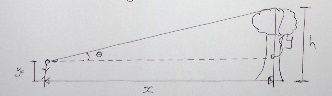
\includegraphics[width=8cm]{./img/clin1.jpg}\\
	$\tan \theta = \cfrac{y}{x}$\\
	$y = x\tan \theta$\\
	$h = y_o + y$
	\end{center}

Help students to prepare a data table as shown below, and then split them up into groups to go collect and record their data and calculate the height of a building. Have them compare their answers and identify sources of error. If possible, obtain the actual height and see how the calculated values compare. This is a great Math Practical for Form IV students! Which professions might use this method of measurement?\\
\begin{center}
\begin{tabular}{|c|c|c||c|c|c|c|} \hline
\multicolumn{3}{|c||}{\textbf{Measurements}} & \multicolumn{4}{c|}{\textbf{Calculations}} \\ \hline
$x$ & $y_o$ & $(90^\circ - \theta)$ & $\theta$ & $\tan \theta$ & $y = x\tan \theta$ & $h = y_o + y$\\
(m) & (m) & ($^\circ$) & ($^\circ$) & & (m) & (m)\\ \hline
&&&&&& \\ \hline
\end{tabular}
\end{center}
\end{itemize}

\section{Compass} \label{compass}
\textbf{How to Make:} Use a strip of folded paper with holes at various lengths along the paper. Keep one pen secure at one end and use another pen or pencil to trace a circle. Alternatively, use a length of string tied around two pens at either end. Unroll the connecting string to the desired length and secure one pen to be the center of the circle and use the other to trace the circumference.\\

\noindent\textbf{Uses:}
\begin{itemize}
\item Have each student make one of these paper compasses for taking notes, especially during topics when they need to draw many, many circles. Otherwise they will be sharing coins or compasses and it will take a long time for them to copy your notes.
\end{itemize}

\section{Dice} \label{dice}
\textbf{How to Make:} Take an empty chalk container and write numbers on the sides. Or you can make a box using manila paper, or even make cubes out of bars of soap. Have your students help to make them - they love helping with these projects.\\

\noindent\textbf{Uses:}
\begin{itemize}
\item \emph{Probability}: Students love to play and see probability happen rather than just memorizing formulas. Chart the results of using dice. Then discover the formulas of probability.
\item \emph{Coordinate Geometry}: Use dice to generate random numbers for plotting points, graphing lines, etc.
\item \emph{Numbers}: Use random numbers to drill students on multiplication, addition, fractions, decimals, etc.
\end{itemize}

\section{Dominoes} \label{dominoes}
\textbf{How to Make:} Use a little rectangular paper marked in 2 sections. For example, one section has a number four and the other section has a number six.\\

\noindent\textbf{Uses:}
\begin{itemize}
\item From the example, the ordered pair $(4,6)$ can be written. This random point can be graphed on a \nameref{cartesianplane}.
\item These domino cards can also be used for random pairing of numbers as they learn multiplication tables. These must be drilled in many ways, because older students often still use tables on their exercise books, which will not be available to them during exams.
\end{itemize}

\section{Flash Cards} \label{flashcards}
\textbf{How to Make:} Small cards or paper rectangles can be used.\\

\noindent\textbf{Uses:}
\begin{itemize}
\item Students enjoy playing \nameref{aroundtheworld} in the classroom as multiplication tables are drilled.
\item These cards can be used for board races with 6 or more students at the board responding to the flash card. All the students at their desks can also be responding to the question.
\item Use flashcards with pictures or math terms written on them to quiz students on new terminology.
\end{itemize}

\section{Fractions and Decimals} \label{fracsanddecs}
\textbf{How to Make:} Empty water bottles are excellent for teaching fractions and are very meaningful. Each student can supply an empty bottle from home to use during class.

Sticks can be put to better use in math class than for discipline. Have the students collect them and they will become fractions. Now the students have an object of one-half, one-third or any fractional component. After students understand these fraction concepts, there are activities on \nameref{fractions} which may be used. \\

\noindent\textbf{Uses:}
\begin{itemize}
\item Have students fill up half a bottle, one-third of a bottle, etc. Students can continue to add one-half and one-half to get a full bottle as they work together in pairs with their bottles of water.
\item Students can then subtract with fractions in the same way. What learning! Have them write all the fraction addition and subtraction problems they have solved. Creating fraction equations with the sticks and then solving them will help the students understand the operations on fractions.
\item Relating these fractions to cooking will be very practical and meaningful. To cook, one measures one cup, a half cup, a third cup, etc. What happens when we must cook for twice the number of people?
\item Convert these learning exercises to decimals. Students need to see and touch 0.5 or 0.3 or 0.25 to learn the meaning of it. Sometimes even money can be used.
\end{itemize}

\section{Geoboard} \label{geoboard}
\textbf{How to Make:} Gather nails and left-over square slabs of wood of various sizes from a local carpenter, or have students supply these items from their homes. Place nails in a grid at one inch or 2 centimeters apart from each other, across and down to get a square. The number of nails used will be based on the size of the piece of wood. A size of 10 by 10 is excellent. 

Many times a carpenter will share these items to increase the learning experience of students, or your school may share. The carpenter knows how often numbers are used in his profession! Every student can build a geoboard, or one geoboard for a group of 4 students. It is good to involve the parents in a day school.

	\begin{center}
	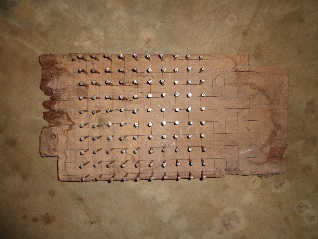
\includegraphics[width=5cm]{./img/gb1.jpg}
	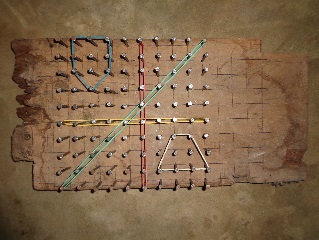
\includegraphics[width=5cm]{./img/gb2.jpg}
	\end{center}

\noindent\textbf{Uses:}
\begin{itemize}
\item \emph{Perimeter}: The formula for perimeter around any size rectangle can be demonstrated. For example, for a rectangle of 5 inches by 4 inches, one can use rubber bands to mark off the given dimensions, and then one can count 18 units of perimeter to see that:
\begin{center}
$2 \times \text{Length} + 2 \times \text{Width} = \text{Perimeter}$
\end{center}
\item \emph{Area}: The formula for area can be demonstrated by marking a rectangle of 5 inches by 4 inches or any dimension. Use rubber bands to mark the square. Count the square units in the surface of the rectangle - it will be 20 square units. This will allow students to discover the formula:
\begin{center}
$\text{Length} \times \text{Width} = \text{Area} $
\end{center}
\item \emph{Coordinate Geometry}: Lines can be graphed on a \nameref{cartesianplane}. First mark the $x$-axis and $y$-axis. It is good to use different colors of rubber bands (yellow for $y$-axis and red for $x$-axis). Use little dots of paper to plot the points. After plotting 3 or 4 points, use a rubber band to connect them. The students enjoy such hands on activities.

After a line is plotted, one can demonstrate slope, or gradient. Slope is the change of $y$ over change of $x$ and can be counted and demonstrated on a geoboard.

Parallel lines can be placed on a geoboard with rubber bands. Then one can use the points to see that the slopes are equal for these two lines. Also try it with perpendicular lines.
\item \emph{Relations and Functions}: After tables of values are created, students can plot them on the geoboard. Begin by graphing the line using two points from the table. Then one can find the domain and range. The inverse can be discovered and discussed as well. All of this on relations can also be applied to functions.
\end{itemize}

\section{Globe} \label{globe}
\textbf{How to Make:} Have students make spheres by binding thin strips of bamboo together with string. Make sure they have axes through the center and a few outer rings. You can fill in the empty sections with paper to illustrate various angles within the sphere.\\

\noindent\textbf{Uses:}
\begin{itemize}
\item \emph{Earth as a Sphere}: Use the spheres in class to teach students about longitude and latitude, great circles, the equator and prime meridian, and various angles measured within the sphere. Color-code different properties and have students try to label them.
\end{itemize}

\section{Number Line} \label{numberline}
\textbf{How to Make:} Create a number line in a variety of ways. The best may be a piece of string or ruler. Then have numbers written on little dots that can be placed along the number line in positive and negative directions.

Students can be a number line in class. Thy can hold a positive or negative number. Involvement is the best way to learn. 

Number lines can be drawn outside in the dirt for even more interactive learning.\\

\noindent\textbf{Uses:}
\begin{itemize}
\item Use the ``hopping method'' of movement as students process $-3 + 1 = -2$. Have one student at a time stand in front of the student number line and hop to the left and right to add and subtract integers. It is good to create a hopping song while learning these negative integers for addition and subtraction. 
\item Inequalities are graphed on a \nameref{numberline}. These graphs are the stepping stone to graphing on an $x$-$y$ plane. It also demonstrates which numbers are larger or smaller. Students need to see to understand such concepts of greater than or less than.
\end{itemize}

\section{Protractor} \label{protractor}
\textbf{How to Make:} Take a square piece of paper and fold it in half into two vertical rectangles (picture 1). Take the top right corner and fold it down to the center line (picture 2). Next, bring the bottom left corner to the same point on the center line so that the left edge meets along the edge just folded (not pictured). Then fold up the lower edge to make the bottom triangle (picture 3). Finally tuck the bottom triangle inside (picture 4). Leave the triangle folded like this, or unfold (picture 5) to view the angles created. Label the angles as shown - this protractor produces angles of $15^\circ$, $30^\circ$, $45^\circ$, $60^\circ$, $75^\circ$, $90^\circ$, $120^\circ$ and $135^\circ$.

	\begin{center}
	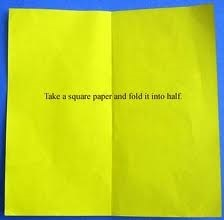
\includegraphics[width=5cm]{./img/prot1.jpg}
	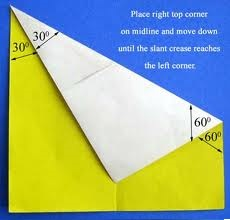
\includegraphics[width=5cm]{./img/prot2.jpg}
	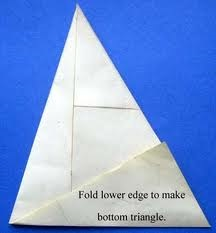
\includegraphics[width=5cm]{./img/prot3.jpg}
	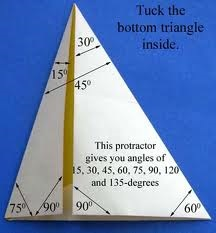
\includegraphics[width=5cm]{./img/prot4.jpg}
	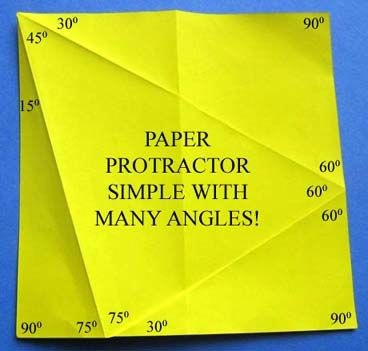
\includegraphics[width=5cm]{./img/prot5.jpg}
	\end{center}

\noindent\textbf{Uses:}
\begin{itemize}
\item \emph{Geometry}: Students can use the paper protractor to construct various acute, obtuse, right and reflex angles.
\end{itemize}

\section{Spinners} \label{spinners}
\textbf{How to Make:} Gather a sheet of paper or cardboard, a pen\slash pencil, paper clip, \nameref{protractor} and \nameref{compass}.

Draw a circle on the paper using the compass. Use the protractor to divide the circle into a desired number of equal-sized sections (have students determine the angle necessary for each section based on the number of sections desired). Label each section with a number, color or some other identifier. Hold the pen\slash pencil in the center of the circle with the paper clip free to spin between it and the paper. Flick the paper clip to start the spinner and see where it lands.\\

\noindent\textbf{Uses:}
\begin{itemize}
\item \emph{Probability}: Create a spinner with different-sized sections and have students determine the probability that it will land on a given one. Conduct several trials to lead students to discover formulas for probability.
\item \emph{Fractions and Decimals}: Label each section with a different fraction or decimal. Or divide the spinner into unequal sections and label each one according to its fraction of the whole circle. Have students perform operations on fractions and decimals that the spinner lands on.
\end{itemize}


\section{Three-Dimensional Objects} \label{3dfigstools}
\textbf{How to Make:} Use paper or a wire grid to construct cylinders, prisms and pyramids. Use empty cardboard boxes or chalk boxes to demonstrate interior angles formed by various planes. Use old Nido and oatmeal tins as cylinders.\\

\noindent\textbf{Uses:}
\begin{itemize}
\item Students get great enjoyment out of constructing these three-dimensional objects themselves. Use them to derive formulas on surface area and volume.
\item Tape a sheet of paper around a large cylindrical tin and use circular lids to show how to derive the surface area of a cylinder.
\item See more in Topics and Activities for the Form IV topic of \nameref{3dfigsactivities}.
\end{itemize}

\chapter{Form I-IV Topics and Activities}

\section{Form I}

	\subsection{Numbers (I)} \label{numbers}
	\begin{itemize}
	\item\nameref{flashcards} can be used to illustrate base ten numeration, as well as reinforce simple arithmetic. Use them to play \nameref{games} such as \nameref{aroundtheworld} to help students master their times tables.
	\item Use a \nameref{numberline} to show addition and subtraction of integers. Using students as the number line is a great way to involve them in the lesson. \nameref{toka} is a great game for students to practice using a number line.
	\item Operations on integers (BODMAS) can be taught using games such as \nameref{fourfours} and \nameref{24squares}.
	\item Be conscious of problem-solving methods common in Tanzanian primary schools for topics such as GCF and LCM which may be instilled in the students. 
	\end{itemize}
	
	\subsection{Fractions} \label{fractions}
	\begin{itemize}
	\item See the Hands-on Tools section for how to make \nameref{fracsanddecs}.
	\item Represent fractions using bottles, sticks, colored circles, etc.
	\item Have a class-wide ``Mock Market'', where students buy and sell fractions of quantities of items such as rice, flour, oil, milk, etc. Can they adjust the prices according to the fractions purchased?
	\item See more \nameref{games} such as \nameref{memory}, \nameref{20questions}, \nameref{guesswho} and \nameref{snap}, as well as \nameref{classacts} on \nameref{classactsfracsdecs}.
	\end{itemize}
	
	\subsection{Decimals and Percentages} \label{decspercents}
	\begin{itemize}
	\item See the Hands-on Tools section for how to make \nameref{fracsanddecs}.
	\item Create movable numbers on manila paper to show that decimal points must be lined up for addition and subtraction.
	\item Play a decimals and percentages \nameref{bingo} game. The students fill their cards with numbers in one form (e.g. decimals) and the teacher calls out numbers in another form (e.g. percentages). Students must first convert the number before being able to cover spaces on their boards. Play this game with fractions as well.
	\item Have students calculate their percentage on homework or in-class assignments, based on the number of questions and how many were answered correctly. 
	\item See more \nameref{games} such as \nameref{memory}, \nameref{20questions}, \nameref{guesswho} and \nameref{snap}, as well as \nameref{classacts} on \nameref{classactsfracsdecs}.
	\end{itemize}
	
	\subsection{Units}
	\begin{itemize}
	\item Use tape measures, rulers and metre rulers to show conversions in length.
	\item Use various sized bottles to demonstrate capacity. Show that three 500 mL bottles is the same volume as a single 1.5 L bottle to reinforce multiplication of fractions.
	\item Students can create a clock to learn units of time.
	\end{itemize}
	
	\subsection{Approximations}
	\begin{itemize}
	\item \nameref{flashcards} can be used to create movable numbers for teaching significant figures.
	\item Have students guess how many pieces of candy are in a small jar. The student who gets closest to the correct number wins the candy!
	\item Estimate the number of students in each stream of every form to approximate the total students at school. Compare this to the actual total. Is it a good estimate?
	\item Ask students to approximate how much corn can be yielded from an acre of farmland. How many acres would be needed for a certain desired profit?
	\end{itemize}
	
	\subsection{Geometry} \label{geometry}
	\begin{itemize}
	\item Use a \nameref{geoboard} to create lines and various polygons and angles.
	\item Circles can be drawn on the ground using a string radius. Students can construct their own circles by making their own \nameref{compass}.
	\item Students can create their own \nameref{protractor} to construct various angles.
	\item Salama says: students act out points, lines and angles using their arms.
	\item Cut out a large triangle having any dimensions. Label each angle and then cut out and tape them together on the board to show that they form a straight line and thus add up to $180^\circ$. Repeat for different polygons to discover formulas for finding interior and exterior angles.
	\item See \nameref{games} such as \nameref{aroundtheworld} and \nameref{battleship}, as well as \nameref{classacts} on \nameref{classactsgeo}.
		\end{itemize}
	
	\subsection{Algebra} \label{algebra}
	\begin{itemize}
	\item Bring a bucket of apples and bananas. Apples represent the ``a'' and bananas represent ``b''. Unlike
objects cannot be added.
	\item Colored chalk can be used. Red and blue cannot be added together.
	\item Use a scale to represent both sides of the equation. If something is added or subtracted to one side, it must be done the same to the other side to maintain balance.
	\item Use cards by writing the variable on one side and its value on the other. When the equation has been solved, the variable reveals its identity by flipping over.
	\item See more ideas in \nameref{classacts} on \nameref{classactsalgebra}.
	\end{itemize}
	
	\subsection{Numbers (II)}
	\begin{itemize}
	\item A \nameref{numberline} is the best tool for teaching numbers, even fractions that are rational numbers.
	\end{itemize}
	
	\subsection{Ratio, Profit and Loss}
	\begin{itemize}
	\item Ratio can be taught with objects to show that Juma gets 2 items for every 3 items that Mary receives.
	\item Show profit and loss through a bottle cap business demonstration, for a given buying price and selling price per bottle cap.
	\item Have students investigate ratios of different body parts. See more in \nameref{classacts} on \nameref{classactsratio}.
	\end{itemize}
	
	\subsection{Coordinate Geometry}
	\begin{itemize}
	\item See the section on Form IV \nameref{coordgeo}
	\end{itemize}
	
	\subsection{Perimeter and Area}
	\begin{itemize}
	\item See the section on Form IV \nameref{areaper}
	\end{itemize}

\section{Form II}

	\subsection{Exponents and Radicals}
	\begin{itemize}
	\item Use \nameref{flashcards} with ``x'' written on them to show that multiplying four of these is equal to ``x'' to the fourth power. 
	\item Add and remove cards in the numerator and denominator to demonstrate the laws of exponents in this way.
	\item Guide students to make tables or posters of the laws of exponents to be posted around the classroom.
	\end{itemize}
	
	\subsection{Algebra}
	\begin{itemize}
	\item Use colored chalk to teach BODMAS.
	\item Factor trees can be helpful when teaching factorization.
	\end{itemize}
	
	\subsection{Quadratic Equations}
	\begin{itemize}
	\item Use crazy names for variables so that students do not combine different variables.
	\item Use a song to help students remember the quadratic formula.
	\end{itemize}
	
	\subsection{Logarithms}
	\begin{itemize}
	\item Help students create charts of the laws of logarithms. These can be hung around the classroom for easy reference.
	\item Ensure students get some practice using four figure tables to solve problems as this is often required on the NECTA exams.
	\end{itemize}
	
	\subsection{Congruence} \label{congruence}
	\begin{itemize}
	\item Draw pairs of various congruent shapes on cards and play \nameref{games} such as \nameref{memory} and \nameref{snap} to get students to identify congruent pairs.
	\item Use origami paper to show how folding squares can produce different congruent shapes.
	\end{itemize}
	
	\subsection{Similarity} \label{similarity}
	\begin{itemize}
	\item Use \nameref{games} such as \nameref{memory} and \nameref{snap} to help students identify and pair off similar figures.
	\item Construct a 2-D house out of cut out triangles and rectangles. Then have students cut out a set of shapes that are similar to the ones you used, and another set which are not similar. Which house better resembles the one you made?
	\end{itemize}
	
	\subsection{Geometrical Transformations}
	\begin{itemize}
	\item Use a \nameref{geoboard} or an x-y plane in the ground to show rotation, reflections, etc.
	\item Students can be used to demonstrate rotation, reflection and translation.
	\item Use bottle caps to show original and transformed shapes side-by-side. See more in \nameref{classacts} on \nameref{classactscoordgeo}.
	\end{itemize}
	
	\subsection{Pythagoras Theorem}
	\begin{itemize}
	\item Help students derive Pythagoras Theorem by using a right triangle made with squares acting as each side. Use the areas of the squares to show that $a^2 + b^2 = c^2$.
	\item Demonstrate a proof of Pythagoras Theorem using a  square sheet of paper folded so that each side is split into lengths of $a$ and $b$, creating an inner square of side length $c$.
	\end{itemize}
	
	\subsection{Trigonometry}
	\begin{itemize}
	\item See the section on Form IV \nameref{trig}.
	\end{itemize}
	
	\subsection{Sets}
	\begin{itemize}
	\item Construct a tangible Venn diagram to place movable shapes, colored objects, etc.
	\item Demonstrate sets and subsets using playing cards, \nameref{dominoes}, dinner ware or even students themselves!
	\end{itemize}
	
	\subsection{Statistics}
	\begin{itemize}
	\item See the section on Form III \nameref{statistics}.
	\end{itemize}

\section{Form III}

	\subsection{Relations} \label{relations}
	\begin{itemize}
	\item Use \nameref{dice} and \nameref{dominoes} for forming Domain and Range sets.
	\item Use a \nameref{geoboard} or \nameref{cartesianplane} to graph relations.
	\end{itemize}

	\subsection{Functions} \label{functions}
	\begin{itemize}
	\item Teach functions using the ``Function Jiko'' method:
		\begin{itemize}
		\item Functions can be likened to cooking ugali on a charcoal jiko. The necessary inputs are added to the jiko - these can be grouped together to represent the independent variable, $x$ (i.e. unga and water).
		\item Then ``stuff happends'' to the input - these are the operations on the independent variable such as multiplication, addition, etc. (i.e. stirring and heating). These must be performed in the correct order to receive the desired product.
		\item Finally, the function ``poops out'' its output after all necessary operations are performed - this is the dependent variable, $y$ (i.e. ugali).
		\item Use a real pot, spoon, etc. to demonstrate this concept to the class. Stress the fact that if you change the input, the output is affected accordingly. In a function, every input correlates to exactly one output.
		\end{itemize}
	\item Graph functions on a \nameref{geoboard} or \nameref{cartesianplane}.
	\item Play a \nameref{battleship} game to reinforce graphing different functions. See more \nameref{classacts} on \nameref{classactsfns}.
	
	\end{itemize}

	\subsection{Statistics} \label{statistics}
	\begin{itemize}
	\item Have students collect data on family or fellow students based on age, height, school level, children in the family, etc. They then organize their data in bar graphs, line graphs, pie charts, histograms, frequency distribution tables, etc. Students can also find mean, median and mode by using formulas or approximations from their graphs and tables. This is a great class project or math practical and can also be used as a way to teach the Scientific Method.
	\item Incorporate statistics on HIV\slash AIDS and malaria to increase awareness of the students in their communities.
	\item Use current football stats on well-known teams to excite and engage students.
	\item Arrange students in a line according to height or age to demonstrate median.
	\end{itemize}

	\subsection{Rates and Variations}
	\begin{itemize}
	\item Demonstrate 2:3:5 using blocks, sticks, bottles, etc. so that it will be concrete learning.
	\item Use different sized syringes or tubes to show that the rate of water flow is proportional to the size of the tube opening.
	\item Use practical examples of direct variation, such as opening and closing a faucet (bomba), cooking ugali and studying vs. test performance. Examples of indirect variation include time spent talking on the phone vs. remaining vocha, notes written vs. chalk length, etc. 
	\item Have students sketch graphs of common practical examples of variations without using numbers.
	\item Incorporate formulas from science subjects, such as chemical reaction rates, Ohm's Law, etc.
	\item Ask students to come up with examples on their own to demonstrate comprehension.
	\end{itemize}

	\subsection{Sequences and Series}
	\begin{itemize}
	\item Translate word statements into math expressions (e.g. 4th term is 10 more than the 2nd term).
	\item List many numbers in a sequence to prove the sum formulas.
	\item Use a \nameref{jeopardy}-style game to challenge students' pattern recognition using numerical and geometrical sequences. This is a great tool for developing logical thought processes.
	\item Make colored posters to hang around the classroom highlighting the distinctions between arithmetical and geometrical progressions.
	\item Have students act out sequence patterns. See more in \nameref{classacts} on \nameref{classactsseqser}.
	\end{itemize}

	\subsection{Circles} \label{circlesactivities}
	\begin{itemize}
	\item See the Hands-On Tools section for how to make \nameref{circlestools}.
	\item Play a game to have students stick paper labels to corresponding properties of circles.
	\item Use a clock to sweep out a span of time to represent a sector of a circle.
	\item Cut out circles to draw on for proving circle theorems in class.
	\item Have students draw what each theorem states to reinforce the concept.
	\end{itemize}

	\subsection{Earth as a Sphere}
	\begin{itemize}
	\item Have students make spheres out of bamboo strips. See more in Hands-On Tools for making a \nameref{globe}.
	\item Use globes, if available, or else footballs, basketballs or volleyballs to show students longitude and latitude.
	\end{itemize}

	\subsection{Accounts} \label{accountsactivities}
	\begin{itemize}
	\item Teach the principle of double entry using the ``Accounts Stendi'' method:
		\begin{itemize}
		\item Each account is like a bus stand, having an entrance (Dr.) side and an exit (Cr.) side. 
		\item When a transaction occurs between two accounts, or bus stands, the money must be transported via the Transaction Express.
		\item The bus exits the first stendi, but the driver must ``sign out'' before leaving by writing the Date of the transaction (Date of travel), Particulars (the bus's destination city\slash account), Folio (the corresponding number code for the destination) and Amount (the money being delivered) under the Cr. side (exit) of the departure stendi.
		\item When the bus reaches its destination, the driver must now ``sign in'' by writing the Date, Particulars (city\slash account of origin), Folio (number code for the origin) and Amount under the Dr. side (entrance) of the arrival stendi.
		\item This analogy helps students to see why it is necessary to record each transaction twice in the account books. For example, a Purchase must be recorded for two purposes: to account for the payment of money \emph{from the Cash Account}, and to account for the receipt of goods \emph{into the Purchases Account}.
		\item Make real accounts and a real Transaction Express bus out of manila paper to demonstrate this concept.
		\end{itemize}
	\item Use movable strips of paper as transactions and allow students to come up to the board to place them in the proper accounts.
	\item Have a small duka demonstration with the class. You have a tomato or bottle cap business and need to keep track of purchases, sales, expenses, such as transport and duka monthly rent fees, and want to know if you are making or losing money.
	\item See more in Hands-On Tools for making \nameref{accountstools}.
	\end{itemize}

\section{Form IV}

	\subsection{Coordinate Geometry} \label{coordgeo}
	\begin{itemize}
	\item A \nameref{geoboard} can be used to demonstrate slope, midpoint, parallel and perpendicular lines, etc.
	\item Allow students to create their own \nameref{cartesianplane} out of old calendars, seed bags or whatever they choose.
	\item Use \nameref{dice} to generate random coordinates for practice with plotting points and to make homework or in-class problems on slope, midpoint, distance formula, etc. Make four dice out of manila paper (2 red - one of +'s and -'s, and one of the numbers 1-6, and then 2 blue in the same way). Students roll the dice to find an x-coordinate (blue) and a y-coordinate (red) and then must plot the point on the Cartesian plane.
	\item Help students use Pythagoras Theorem to derive the distance formula.
	\item Play a \nameref{battleship} game to help students read and plot points.
	\item Have students create different shapes on a coordinate plane by plotting bottle caps. See more in \nameref{classacts} on \nameref{classactscoordgeo}.
	\end{itemize}

	\subsection{Area and Perimeter} \label{areaper}
	\begin{itemize}
	\item Use a \nameref{geoboard} to help students discover formulas of area and perimeter for squares and rectangles.
	\item Using graph paper, have students cut out rectangles having an area of 48 square units. How many different sets of dimensions be used to generate this area?
	\item \nameref{circlestools}, such as bike wheels, can be used to show circumference and also to measure the perimeter around the school or a classroom.
	\item Use string to measure the circumference and diameter of a circle, and to derive $\pi$.
	\item Gather several small circles or cylindrical items of various sizes. Trace the circular outlines on graph paper and for each one, count the number of squares that make up the area and the number of units of length of the radius. Tabulate the results. Can you discover a relationship between radius and area for different sized circles?
	\item Students make various polygons using a \nameref{geoboard} or cutting them out of paper, and then use the shapes to discover formulas.
	\item Have students draw polygons on graph paper (or create their own graph paper) to discover relations between areas of similar figures.
	\end{itemize}

	\subsection{Three-Dimensional Figures} \label{3dfigsactivities}
	\begin{itemize}
	\item See the Hands-On Tools section for how to make \nameref{3dfigstools}.
	\item Have a challenge to see who can identify the most 3-dimensional objects in the classroom.
	\item Use hollow containers or objects that can be opened to see interior angles and planes.
	\item Do a design challenge with students. See more in \nameref{classacts} on \nameref{classacts3d}.
	\end{itemize}

	\subsection{Probability}
	\begin{itemize}
	\item Use \nameref{dice}, playing cards, coins, bottle caps, \nameref{flashcards}, \nameref{spinners}, fruits or any objects to demonstrate probability.
	\item Have students determine the probability of selecting a boy from the class, or two boys. Does the result change if the first one goes outside before the next selection is made?
	\item Relate to genetics in Biology, or incorporate data on HIV\slash AIDS and malaria to increase awareness.
	\item Use a probability line to teach key probability terms and to apply probability to real-life situations. See more in \nameref{classacts} on \nameref{classactsprob}.
	\end{itemize}

	\subsection{Trigonometry} \label{trig}
	\begin{itemize}
	\item Guide students to develop tables of values of trig ratios for special angles for $-360^\circ \leq \theta \leq 360^\circ$ and then use them to graph $\sin$, $\cos$ and $\tan$ functions.
	\item Play a \nameref{bingo} game using trig ratios for some special angles. Instead of B-I-N-G-O, column headers are $\sin$, $\cos$ and $\tan$. Students fill their cards with various values under each trig function, and the teacher calls out a particular trig function and angle. For example, the teacher calls, ``$\sin 30^\circ$'' and students having a ``0.5'' under their $\sin$ column get to cover that space.
	\item Have students create a \nameref{clinometer} to see the application of trigonometry in determining the height of a building or tall tree.
	\end{itemize}

	\subsection{Vectors}
	\begin{itemize}
	\item Use colored origami paper cranes or cut out airplanes to use as points on a \nameref{cartesianplane}. The birds or planes start at one point and travel in a specified direction towards the destination point.
	\item Relate to applications in Physics.
	\item Use colored chalk to show that unlike components cannot be combined.
	\end{itemize}

	\subsection{Matrices and Transformations}
	\begin{itemize}
	\item Charts and colored chalk must be used to demonstrate operations on matrices.
	\item Attach a string to the origin and stretch it out to an object to show rotation about the origin.
	\item Use mirrors or spoons to show reflection.
	\item Use bottle caps to show original and transformed shapes side-by-side. See more in \nameref{classacts} on \nameref{classactscoordgeo}.
	\end{itemize}

	\subsection{Linear Programming}
	\begin{itemize}
	\item A \nameref{geoboard} can be used to demonstrate maximum and minimum.
	\item Drill students on how to generate constraints based on the word problems. Use tables to organize information. This requires the most practice as students are not familiar with many English terms.
	\item Make a math vocab list of key terms such as ``at least,'' ``at most,'' ``no fewer than,'' ``not more than,'' ``minimum'' and ``maximum.''
	\end{itemize}


% Mathematics Hands-On Activities
\part{Hands-On Activities}

% Form I
\chapter{Mathematics Activities for Form I}
%\section{Numbers (I)}

\begin{multicols}{2}


\section*{}


\subsection{}

\begin{center}
\includegraphics[width=0.4\textwidth]{./img/.png}
\end{center}

\begin{description*}
%\item[Subtopic:]{}
\item[Materials:]{}
\item[Setup:]{}
\item[Procedure:]{}
\item[Hazards:]{}
\item[Questions:]{}
\item[Observations:]{}
\item[Theory:]{}
\item[Applications:]{}
\item[Notes:]{}
\end{description*}

%==================================================================================================%


\end{multicols}

\pagebreak
%\section{Fractions}

\begin{multicols}{2}


\section*{}


\subsection{}

\begin{center}
\includegraphics[width=0.4\textwidth]{./img/.png}
\end{center}

\begin{description*}
%\item[Subtopic:]{}
\item[Materials:]{}
\item[Setup:]{}
\item[Procedure:]{}
\item[Hazards:]{}
\item[Questions:]{}
\item[Observations:]{}
\item[Theory:]{}
\item[Applications:]{}
\item[Notes:]{}
\end{description*}

%==================================================================================================%


\end{multicols}

\pagebreak
%\section{Decimals and Percentages}

\begin{multicols}{2}


\section*{}


\subsection{}

\begin{center}
\includegraphics[width=0.4\textwidth]{./img/.png}
\end{center}

\begin{description*}
%\item[Subtopic:]{}
\item[Materials:]{}
\item[Setup:]{}
\item[Procedure:]{}
\item[Hazards:]{}
\item[Questions:]{}
\item[Observations:]{}
\item[Theory:]{}
\item[Applications:]{}
\item[Notes:]{}
\end{description*}

%==================================================================================================%


\end{multicols}

\pagebreak
%\section{Units}

\begin{multicols}{2}


\section*{}


\subsection{}

\begin{center}
\includegraphics[width=0.4\textwidth]{./img/.png}
\end{center}

\begin{description*}
%\item[Subtopic:]{}
\item[Materials:]{}
\item[Setup:]{}
\item[Procedure:]{}
\item[Hazards:]{}
\item[Questions:]{}
\item[Observations:]{}
\item[Theory:]{}
\item[Applications:]{}
\item[Notes:]{}
\end{description*}

%==================================================================================================%


\end{multicols}

\pagebreak
%\section{Approximations}

\begin{multicols}{2}


\section*{}


\subsection{}

\begin{center}
\includegraphics[width=0.4\textwidth]{./img/.png}
\end{center}

\begin{description*}
%\item[Subtopic:]{}
\item[Materials:]{}
\item[Setup:]{}
\item[Procedure:]{}
\item[Hazards:]{}
\item[Questions:]{}
\item[Observations:]{}
\item[Theory:]{}
\item[Applications:]{}
\item[Notes:]{}
\end{description*}

%==================================================================================================%


\end{multicols}

\pagebreak
%\section{Geometry}

\begin{multicols}{2}


\section*{}


\subsection{}

\begin{center}
\includegraphics[width=0.4\textwidth]{./img/.png}
\end{center}

\begin{description*}
%\item[Subtopic:]{}
\item[Materials:]{}
\item[Setup:]{}
\item[Procedure:]{}
\item[Hazards:]{}
\item[Questions:]{}
\item[Observations:]{}
\item[Theory:]{}
\item[Applications:]{}
\item[Notes:]{}
\end{description*}

%==================================================================================================%


\end{multicols}

\pagebreak
%\section{Algebra}

\begin{multicols}{2}


\section*{}


\subsection{}

\begin{center}
\includegraphics[width=0.4\textwidth]{./img/.png}
\end{center}

\begin{description*}
%\item[Subtopic:]{}
\item[Materials:]{}
\item[Setup:]{}
\item[Procedure:]{}
\item[Hazards:]{}
\item[Questions:]{}
\item[Observations:]{}
\item[Theory:]{}
\item[Applications:]{}
\item[Notes:]{}
\end{description*}

%==================================================================================================%


\end{multicols}

\pagebreak
%\section{Numbers (II)}

\begin{multicols}{2}


\section*{}


\subsection{}

\begin{center}
\includegraphics[width=0.4\textwidth]{./img/.png}
\end{center}

\begin{description*}
%\item[Subtopic:]{}
\item[Materials:]{}
\item[Setup:]{}
\item[Procedure:]{}
\item[Hazards:]{}
\item[Questions:]{}
\item[Observations:]{}
\item[Theory:]{}
\item[Applications:]{}
\item[Notes:]{}
\end{description*}

%==================================================================================================%


\end{multicols}

\pagebreak
%\section{Ratio, Profit and Loss}

\begin{multicols}{2}


\section*{}


\subsection{}

\begin{center}
\includegraphics[width=0.4\textwidth]{./img/.png}
\end{center}

\begin{description*}
%\item[Subtopic:]{}
\item[Materials:]{}
\item[Setup:]{}
\item[Procedure:]{}
\item[Hazards:]{}
\item[Questions:]{}
\item[Observations:]{}
\item[Theory:]{}
\item[Applications:]{}
\item[Notes:]{}
\end{description*}

%==================================================================================================%


\end{multicols}

\pagebreak
%\section{Coordinate Geometry}

\begin{multicols}{2}


\section*{}


\subsection{}

\begin{center}
\includegraphics[width=0.4\textwidth]{./img/.png}
\end{center}

\begin{description*}
%\item[Subtopic:]{}
\item[Materials:]{}
\item[Setup:]{}
\item[Procedure:]{}
\item[Hazards:]{}
\item[Questions:]{}
\item[Observations:]{}
\item[Theory:]{}
\item[Applications:]{}
\item[Notes:]{}
\end{description*}

%==================================================================================================%


\end{multicols}

\pagebreak
%\section{Perimeter and Area}

\begin{multicols}{2}


\section*{}


\subsection{}

\begin{center}
\includegraphics[width=0.4\textwidth]{./img/.png}
\end{center}

\begin{description*}
%\item[Subtopic:]{}
\item[Materials:]{}
\item[Setup:]{}
\item[Procedure:]{}
\item[Hazards:]{}
\item[Questions:]{}
\item[Observations:]{}
\item[Theory:]{}
\item[Applications:]{}
\item[Notes:]{}
\end{description*}

%==================================================================================================%


\end{multicols}

\pagebreak

% Form II
\chapter{Mathematics Activities for Form II}
%\section{Exponents and Radicals}

\begin{multicols}{2}


\section*{}


\subsection{}

\begin{center}
\includegraphics[width=0.4\textwidth]{./img/.png}
\end{center}

\begin{description*}
%\item[Subtopic:]{}
\item[Materials:]{}
\item[Setup:]{}
\item[Procedure:]{}
\item[Hazards:]{}
\item[Questions:]{}
\item[Observations:]{}
\item[Theory:]{}
\item[Applications:]{}
\item[Notes:]{}
\end{description*}

%==================================================================================================%


\end{multicols}

\pagebreak
%\section{Algebra}

\begin{multicols}{2}


\section*{}


\subsection{}

\begin{center}
\includegraphics[width=0.4\textwidth]{./img/.png}
\end{center}

\begin{description*}
%\item[Subtopic:]{}
\item[Materials:]{}
\item[Setup:]{}
\item[Procedure:]{}
\item[Hazards:]{}
\item[Questions:]{}
\item[Observations:]{}
\item[Theory:]{}
\item[Applications:]{}
\item[Notes:]{}
\end{description*}

%==================================================================================================%


\end{multicols}

\pagebreak
%\section{Quadratic Equations}

\begin{multicols}{2}


\section*{}


\subsection{}

\begin{center}
\includegraphics[width=0.4\textwidth]{./img/.png}
\end{center}

\begin{description*}
%\item[Subtopic:]{}
\item[Materials:]{}
\item[Setup:]{}
\item[Procedure:]{}
\item[Hazards:]{}
\item[Questions:]{}
\item[Observations:]{}
\item[Theory:]{}
\item[Applications:]{}
\item[Notes:]{}
\end{description*}

%==================================================================================================%


\end{multicols}

\pagebreak
%\section{Logarithms}

\begin{multicols}{2}


\section*{}


\subsection{}

\begin{center}
\includegraphics[width=0.4\textwidth]{./img/.png}
\end{center}

\begin{description*}
%\item[Subtopic:]{}
\item[Materials:]{}
\item[Setup:]{}
\item[Procedure:]{}
\item[Hazards:]{}
\item[Questions:]{}
\item[Observations:]{}
\item[Theory:]{}
\item[Applications:]{}
\item[Notes:]{}
\end{description*}

%==================================================================================================%


\end{multicols}

\pagebreak
%\section{Congruence}

\begin{multicols}{2}


\section*{}


\subsection{}

\begin{center}
\includegraphics[width=0.4\textwidth]{./img/.png}
\end{center}

\begin{description*}
%\item[Subtopic:]{}
\item[Materials:]{}
\item[Setup:]{}
\item[Procedure:]{}
\item[Hazards:]{}
\item[Questions:]{}
\item[Observations:]{}
\item[Theory:]{}
\item[Applications:]{}
\item[Notes:]{}
\end{description*}

%==================================================================================================%


\end{multicols}

\pagebreak
%\section{Similarity}

\begin{multicols}{2}


\section*{}


\subsection{}

\begin{center}
\includegraphics[width=0.4\textwidth]{./img/.png}
\end{center}

\begin{description*}
%\item[Subtopic:]{}
\item[Materials:]{}
\item[Setup:]{}
\item[Procedure:]{}
\item[Hazards:]{}
\item[Questions:]{}
\item[Observations:]{}
\item[Theory:]{}
\item[Applications:]{}
\item[Notes:]{}
\end{description*}

%==================================================================================================%


\end{multicols}

\pagebreak
%\section{Geometrical Transformations}

\begin{multicols}{2}


\section*{}


\subsection{}

\begin{center}
\includegraphics[width=0.4\textwidth]{./img/.png}
\end{center}

\begin{description*}
%\item[Subtopic:]{}
\item[Materials:]{}
\item[Setup:]{}
\item[Procedure:]{}
\item[Hazards:]{}
\item[Questions:]{}
\item[Observations:]{}
\item[Theory:]{}
\item[Applications:]{}
\item[Notes:]{}
\end{description*}

%==================================================================================================%


\end{multicols}

\pagebreak
%\section{Pythagoras Theorem}

\begin{multicols}{2}


\section*{}


\subsection{}

\begin{center}
\includegraphics[width=0.4\textwidth]{./img/.png}
\end{center}

\begin{description*}
%\item[Subtopic:]{}
\item[Materials:]{}
\item[Setup:]{}
\item[Procedure:]{}
\item[Hazards:]{}
\item[Questions:]{}
\item[Observations:]{}
\item[Theory:]{}
\item[Applications:]{}
\item[Notes:]{}
\end{description*}

%==================================================================================================%


\end{multicols}

\pagebreak
%\section{Trigonometry}

\begin{multicols}{2}


\section*{}


\subsection{}

\begin{center}
\includegraphics[width=0.4\textwidth]{./img/.png}
\end{center}

\begin{description*}
%\item[Subtopic:]{}
\item[Materials:]{}
\item[Setup:]{}
\item[Procedure:]{}
\item[Hazards:]{}
\item[Questions:]{}
\item[Observations:]{}
\item[Theory:]{}
\item[Applications:]{}
\item[Notes:]{}
\end{description*}

%==================================================================================================%


\end{multicols}

\pagebreak
%\section{Sets}

\begin{multicols}{2}


\section*{}


\subsection{}

\begin{center}
\includegraphics[width=0.4\textwidth]{./img/.png}
\end{center}

\begin{description*}
%\item[Subtopic:]{}
\item[Materials:]{}
\item[Setup:]{}
\item[Procedure:]{}
\item[Hazards:]{}
\item[Questions:]{}
\item[Observations:]{}
\item[Theory:]{}
\item[Applications:]{}
\item[Notes:]{}
\end{description*}

%==================================================================================================%


\end{multicols}

\pagebreak
%\section{Statistics}

\begin{multicols}{2}


\section*{}


\subsection{}

\begin{center}
\includegraphics[width=0.4\textwidth]{./img/.png}
\end{center}

\begin{description*}
%\item[Subtopic:]{}
\item[Materials:]{}
\item[Setup:]{}
\item[Procedure:]{}
\item[Hazards:]{}
\item[Questions:]{}
\item[Observations:]{}
\item[Theory:]{}
\item[Applications:]{}
\item[Notes:]{}
\end{description*}

%==================================================================================================%


\end{multicols}

\pagebreak

% Form III
\chapter{Mathematics Activities for Form III}
%\section{Relations}

\begin{multicols}{2}


\section*{}


\subsection{}

\begin{center}
\includegraphics[width=0.4\textwidth]{./img/.png}
\end{center}

\begin{description*}
%\item[Subtopic:]{}
\item[Materials:]{}
\item[Setup:]{}
\item[Procedure:]{}
\item[Hazards:]{}
\item[Questions:]{}
\item[Observations:]{}
\item[Theory:]{}
\item[Applications:]{}
\item[Notes:]{}
\end{description*}

%==================================================================================================%


\end{multicols}

\pagebreak
%\section{Functions}

\begin{multicols}{2}


\section*{}


\subsection{}

\begin{center}
\includegraphics[width=0.4\textwidth]{./img/.png}
\end{center}

\begin{description*}
%\item[Subtopic:]{}
\item[Materials:]{}
\item[Setup:]{}
\item[Procedure:]{}
\item[Hazards:]{}
\item[Questions:]{}
\item[Observations:]{}
\item[Theory:]{}
\item[Applications:]{}
\item[Notes:]{}
\end{description*}

%==================================================================================================%


\end{multicols}

\pagebreak
%\section{Statistics}

\begin{multicols}{2}


\section*{}


\subsection{}

\begin{center}
\includegraphics[width=0.4\textwidth]{./img/.png}
\end{center}

\begin{description*}
%\item[Subtopic:]{}
\item[Materials:]{}
\item[Setup:]{}
\item[Procedure:]{}
\item[Hazards:]{}
\item[Questions:]{}
\item[Observations:]{}
\item[Theory:]{}
\item[Applications:]{}
\item[Notes:]{}
\end{description*}

%==================================================================================================%


\end{multicols}

\pagebreak
%\section{Rates and Variations}

\begin{multicols}{2}


\section*{}


\subsection{}

\begin{center}
\includegraphics[width=0.4\textwidth]{./img/.png}
\end{center}

\begin{description*}
%\item[Subtopic:]{}
\item[Materials:]{}
\item[Setup:]{}
\item[Procedure:]{}
\item[Hazards:]{}
\item[Questions:]{}
\item[Observations:]{}
\item[Theory:]{}
\item[Applications:]{}
\item[Notes:]{}
\end{description*}

%==================================================================================================%


\end{multicols}

\pagebreak
%\section{Sequences and Series}

\begin{multicols}{2}


\section*{}


\subsection{}

\begin{center}
\includegraphics[width=0.4\textwidth]{./img/.png}
\end{center}

\begin{description*}
%\item[Subtopic:]{}
\item[Materials:]{}
\item[Setup:]{}
\item[Procedure:]{}
\item[Hazards:]{}
\item[Questions:]{}
\item[Observations:]{}
\item[Theory:]{}
\item[Applications:]{}
\item[Notes:]{}
\end{description*}

%==================================================================================================%


\end{multicols}

\pagebreak
%\section{Circles}

\begin{multicols}{2}


\section*{}


\subsection{}

\begin{center}
\includegraphics[width=0.4\textwidth]{./img/.png}
\end{center}

\begin{description*}
%\item[Subtopic:]{}
\item[Materials:]{}
\item[Setup:]{}
\item[Procedure:]{}
\item[Hazards:]{}
\item[Questions:]{}
\item[Observations:]{}
\item[Theory:]{}
\item[Applications:]{}
\item[Notes:]{}
\end{description*}

%==================================================================================================%


\end{multicols}

\pagebreak
%\section{Earth as a Sphere}

\begin{multicols}{2}


\section*{}


\subsection{}

\begin{center}
\includegraphics[width=0.4\textwidth]{./img/.png}
\end{center}

\begin{description*}
%\item[Subtopic:]{}
\item[Materials:]{}
\item[Setup:]{}
\item[Procedure:]{}
\item[Hazards:]{}
\item[Questions:]{}
\item[Observations:]{}
\item[Theory:]{}
\item[Applications:]{}
\item[Notes:]{}
\end{description*}

%==================================================================================================%


\end{multicols}

\pagebreak
%\section{Accounts}

\begin{multicols}{2}


\section*{}


\subsection{}

\begin{center}
\includegraphics[width=0.4\textwidth]{./img/.png}
\end{center}

\begin{description*}
%\item[Subtopic:]{}
\item[Materials:]{}
\item[Setup:]{}
\item[Procedure:]{}
\item[Hazards:]{}
\item[Questions:]{}
\item[Observations:]{}
\item[Theory:]{}
\item[Applications:]{}
\item[Notes:]{}
\end{description*}

%==================================================================================================%


\end{multicols}

\pagebreak

% Form IV
\chapter{Mathematics Activities for Form IV}
%\section{Coordinate Geometry}

\begin{multicols}{2}


\section*{}


\subsection{}

\begin{center}
\includegraphics[width=0.4\textwidth]{./img/.png}
\end{center}

\begin{description*}
%\item[Subtopic:]{}
\item[Materials:]{}
\item[Setup:]{}
\item[Procedure:]{}
\item[Hazards:]{}
\item[Questions:]{}
\item[Observations:]{}
\item[Theory:]{}
\item[Applications:]{}
\item[Notes:]{}
\end{description*}

%==================================================================================================%


\end{multicols}

\pagebreak
%\section{Area and Perimeter}

\begin{multicols}{2}


\section*{}


\subsection{}

\begin{center}
\includegraphics[width=0.4\textwidth]{./img/.png}
\end{center}

\begin{description*}
%\item[Subtopic:]{}
\item[Materials:]{}
\item[Setup:]{}
\item[Procedure:]{}
\item[Hazards:]{}
\item[Questions:]{}
\item[Observations:]{}
\item[Theory:]{}
\item[Applications:]{}
\item[Notes:]{}
\end{description*}

%==================================================================================================%


\end{multicols}

\pagebreak
%\section{Three-Dimensional Figures}

\begin{multicols}{2}


\section*{}


\subsection{}

\begin{center}
\includegraphics[width=0.4\textwidth]{./img/.png}
\end{center}

\begin{description*}
%\item[Subtopic:]{}
\item[Materials:]{}
\item[Setup:]{}
\item[Procedure:]{}
\item[Hazards:]{}
\item[Questions:]{}
\item[Observations:]{}
\item[Theory:]{}
\item[Applications:]{}
\item[Notes:]{}
\end{description*}

%==================================================================================================%


\end{multicols}

\pagebreak
%\section{Probability}

\begin{multicols}{2}


\section*{}


\subsection{}

\begin{center}
\includegraphics[width=0.4\textwidth]{./img/.png}
\end{center}

\begin{description*}
%\item[Subtopic:]{}
\item[Materials:]{}
\item[Setup:]{}
\item[Procedure:]{}
\item[Hazards:]{}
\item[Questions:]{}
\item[Observations:]{}
\item[Theory:]{}
\item[Applications:]{}
\item[Notes:]{}
\end{description*}

%==================================================================================================%


\end{multicols}

\pagebreak
%\section{Trigonometry}

\begin{multicols}{2}


\section*{}


\subsection{}

\begin{center}
\includegraphics[width=0.4\textwidth]{./img/.png}
\end{center}

\begin{description*}
%\item[Subtopic:]{}
\item[Materials:]{}
\item[Setup:]{}
\item[Procedure:]{}
\item[Hazards:]{}
\item[Questions:]{}
\item[Observations:]{}
\item[Theory:]{}
\item[Applications:]{}
\item[Notes:]{}
\end{description*}

%==================================================================================================%


\end{multicols}

\pagebreak
%\section{Vectors}

\begin{multicols}{2}


\section*{}


\subsection{}

\begin{center}
\includegraphics[width=0.4\textwidth]{./img/.png}
\end{center}

\begin{description*}
%\item[Subtopic:]{}
\item[Materials:]{}
\item[Setup:]{}
\item[Procedure:]{}
\item[Hazards:]{}
\item[Questions:]{}
\item[Observations:]{}
\item[Theory:]{}
\item[Applications:]{}
\item[Notes:]{}
\end{description*}

%==================================================================================================%


\end{multicols}

\pagebreak
%\section{Matrices and Transformations}

\begin{multicols}{2}


\section*{}


\subsection{}

\begin{center}
\includegraphics[width=0.4\textwidth]{./img/.png}
\end{center}

\begin{description*}
%\item[Subtopic:]{}
\item[Materials:]{}
\item[Setup:]{}
\item[Procedure:]{}
\item[Hazards:]{}
\item[Questions:]{}
\item[Observations:]{}
\item[Theory:]{}
\item[Applications:]{}
\item[Notes:]{}
\end{description*}

%==================================================================================================%


\end{multicols}

\pagebreak
%\section{Linear Programming}

\begin{multicols}{2}


\section*{}


\subsection{}

\begin{center}
\includegraphics[width=0.4\textwidth]{./img/.png}
\end{center}

\begin{description*}
%\item[Subtopic:]{}
\item[Materials:]{}
\item[Setup:]{}
\item[Procedure:]{}
\item[Hazards:]{}
\item[Questions:]{}
\item[Observations:]{}
\item[Theory:]{}
\item[Applications:]{}
\item[Notes:]{}
\end{description*}

%==================================================================================================%


\end{multicols}

\pagebreak


\chapter{Games and Activities for Stimulating Interest in Mathematics} \label{cha:gamesandactivities}
Math must be stimulated by puzzles, games, patterns, activities and other forms of hands-on and interactive learning. An interest in mathematical puzzles generates creative thinking and motivates students in a way that standard textbooks can rarely achieve. Given that the vast majority of Tanzanian students do not have access to any textbooks at all, the importance of interactive learning techniques such as those provided in this section must not be underestimated.

Many of these games and activities reinforce very basic mathematical concepts, so they are a great way to help solidify students' understanding of such crucial topics through a variety of approaches. Given some creative dimension to their learning, students become more enthusiastic about practicing their math skills.

\section{Games} \label{games}

	\subsection{Jeopardy} \label{jeopardy}
	\textbf{Applicable Topics:} Any topic as a review game\\	
	\textbf{Number of Players:} 3-6 Groups\\
	
	\noindent \textbf{How to Play:}\\
	Divide the class into equal groups and allow them to select their own team name. Designate one student from each team as the writer. Select 5 categories (see suggestions below) and write them at the top of the board on the far left. Beneath each category, write 100, 200 and 300, using colored chalk if possible. Each question's point value is based on its difficulty (100 - easy, 200 - average, 300 - difficult). Write a column for each team on the right side of the board and leave the center of the board empty.
	
	The first team selects a question by stating a category and a point value. The teacher writes the problem in the center of the board for all groups to see. Groups work together to solve the problem, but only the designated writer may present the answer. When an answer is found, writers must hold their notebooks high above their heads so that no further changes can be made, and everyone in the group must remain silent. The first group to finish with a correct answer gets the points and may select the next question. However, groups only get \textbf{one} attempt at each question, so if they are wrong, they are finished until the next question. If none of the groups answer correctly, the teacher gets the points! Once a correct answer has been given, have one student come up to the board to show the rest of the class. 
	
	This is a wonderful review game to play before an exam, since it also shows students what topics they need to study.\\
	
	\noindent \textbf{Extensions:}
	
	\noindent JEOPARDY works great as a review game for any topics covered in class. However, it can also be useful for teaching logical thinking skills, and may be incorporated as part of a Math Day-type promotional school event, or a Math and Science Conference or Competition. Here are some suggested categories for such game variants.
	\begin{itemize}
	\item \emph{Pattern Problems} - pattern recognition sequences for progressions of shapes, rotating figures, letters, etc. Give the first 3, students must find the following 2. (e.g. Abcd, eFgh, ijKl, $\_\_\_$, $\_\_\_$)
	\item \emph{Sequence Solvers} - Numerical sequences or series with various rules. Give the first 4, students must find the following 2. (e.g. 1, $\frac{1}{22}$, 333, $\frac{1}{4,444}$, $\_\_\_$, $\_\_\_$)
	\item \emph{Creative Classes} - Write 9 items on the board, mixed together randomly. Groups must find common characteristics among the items to classify them into 3 groups of 3. (e.g. Oxygen, Milk, Water, Pen, Table, Carbon Dioxide, Oil, Air, Rice - \textit{Gases, Liquids, Solids})
	\item \emph{Word Work} - Give students a word that applies to math or science. Groups must make at least four 3-or-more-letter words by re-arranging the letters. (e.g. MATHEMATICS - math, mat, the, them, $\ldots$)
	\item \emph{Design Dilemmas} - Groups must solve design problems using given constraints. For example:
		\begin{itemize}
		\item You must design a rectangular building having a volume of 64 m$^3$. What is the smallest surface area you can use?
		\item You need to fence a farm having an area of 48 m$^2$. What is the smallest length of fence you can use to border the full area of the farm?
		\end{itemize}	 
	\end{itemize}
	
	\subsection{Memory Matching} \label{memory}
	\textbf{Applicable Topics:} \nameref{fractions}, \nameref{decspercents}, \nameref{congruence}, \nameref{similarity}, \nameref{areaper}, \nameref{algebra}\\	
	\textbf{Number of Players:} 2-6\\
	
	\noindent \textbf{How to Play:}\\
	Prepare roughly 10 pairs of cards, with each set being a different pair of congruent shapes. Mix all cards together and place them in a grid, face down. Players take turns turning over 2 cards at a time. If the pair is a match of congruent shapes, they get to keep them and try another pair of cards. If they are not a match, they must turn them face down again, in their same places, and it is the next player's turn to try. The game ends when all cards have been paired off. The player with the most pairs wins.\\
	
	\noindent \textbf{Extensions:}
	\begin{itemize}
	\item Use pairs of similar shapes instead of congruent shapes.
	\item Make pairs of equivalent fractions, decimals or percentages. All students work together to determine if a given pair are equivalent.
	\item Make pairs with one card being a math equation and its pair being the solution. This can be applied to nearly any topic.
	\item Turn the game into a Concentration game. On a big sheet of paper the size of the full grid of cards, write down a math problem, e.g. a pair of simultaneous equations or a problem on area or perimeter. Without students seeing this sheet, cover it with the face down card grid. As students remove successfully paired cards, the picture beneath is revealed, piece by piece. The first student to solve the problem underneath is the winner. They may need to make inferences or assumptions while parts of the board are still covered.
	\end{itemize}
		
	\subsection{Around the World} \label{aroundtheworld}	
	\textbf{Applicable Topics:} \nameref{numbers}, \nameref{fractions}, \nameref{decspercents}, \nameref{geometry}, \nameref{areaper}\\	
	\textbf{Number of Players:} Entire class\\
	
	\noindent \textbf{How to Play:}\\
	Use \nameref{flashcards} to drill basic math operations. The first 2 students stand up next to each other at their desks. The teacher holds up a card, e.g. 5 $\times$ 2. The first students to give the correct answer moves on, the other student sits down. The winner then faces the next student in order, who stands up and another card is drawn. When a player is defeated, he or she must take the seat of the student who beat them. See who can make it the farthest without being beaten. Can anyone make it around the entire classroom and back to their original seat? It is important for the rest of the class to be silent while two players are facing off.\\
	
	\noindent \textbf{Extensions:}
	\begin{itemize}
	\item Instead of operations, have students compete in converting fractions, decimals and percentages.
	\item Show students simple shapes with dimensions and have them state the area or perimeter.
	\item Show students various shapes and they must be first to identify the shape, e.g. pentagon, rhombus, isosceles triangle, etc.
	\end{itemize}
	
	\subsection{BINGO} \label{bingo}
	\textbf{Applicable Topics:} \nameref{numbers}, \nameref{fractions}, \nameref{decspercents}, \nameref{trig}\\	
	\textbf{Number of Players:} Entire class\\
	
	\noindent \textbf{How to Play:}\\
	Each student makes a 4 $\times$ 4 or 5 $\times$ 5 table in their notebook. Students then fill their game card with random numbers from a given range specified by the teacher, e.g. from 1-40, even numbers from 1-100, etc. The teacher then calls out numbers one at a time. If students have that number on their cards, they place a marker (small square of paper) to cover it up. When a player has a full row, column or diagonal covered, they must shout, ``Bingo!'' and the teacher checks to confirm all of the numbers were called. Players then clear their cards and a new game begins.\\
	
	\noindent \textbf{Extensions:}
	\begin{itemize}
	\item Instead of just calling the numbers, give students a short problem that they must solve first. For example, instead of reading ``5,'' write on the board the equation, ``4 $\times$ 3 - 7'' Use this method to review BODMAS.
	\item Drill conversions among fractions, decimals and percentages. Students fill their cards by writing one form (e.g. decimals), but the teacher reads numbers in another form (e.g. fractions). Be sure to tell students what range to select numbers from when filling up their cards.
	\item Apply to trigonometry. Instead of B-I-N-G-O, column headers are $\sin$, $\cos$ and $\tan$. Students fill their cards with various values under each trig function, and the teacher calls out a particular trig function and angle. For example, the teacher calls, ``$\sin 30^\circ$'' and students having a ``0.5'' under their $\sin$ column get to cover that space.
	\end{itemize}
	
	\subsection{Battleship} \label{battleship}
	\textbf{Applicable Topics:} \nameref{coordgeo}, \nameref{geometry}, \nameref{relations}, \nameref{functions}\\	
	\textbf{Number of Players:} 2\\
	
	\noindent \textbf{How to Play:}\\
	Each player makes 2 coordinate planes out of paper or card. Both the $x$ and $y$ axes should span from -5 to 5. Players arrange their papers such that one is standing vertically against a stack of books and the other is resting in front of it on a flat surface, hidden from the view of the other player.
	
	Players secretly place their ships on the flat coordinate plane in front of them. Ships are placed across several coordinate points, but may not be placed on a diagonal. For example, Player 1's battleship is placed horizontally across 4 points, from (-2,-3) to (2,-3). Each player has 5 ships of lengths 2, 3, 3, 4 and 5. Ships should be clearly marked using bottle caps, colored pen or some other indicator and cannot be moved once placed.
	
	Player 1 begins by calling out a coordinate point. If the point lies on one of Player 2's ships, he or she says, ``Hit,'' otherwise it is a ``Miss.'' Player 1 uses his or her vertical coordinate  plane to keep track of hits and misses on Player 2's ships. Players go back and forth until all of one player's ships are sunk.\\
	
	\noindent \textbf{Extensions:}
	\begin{itemize}
	\item Apply to geometry by using shapes instead of ships. Players must hit every corner in order to sink the shape.
	\item Apply to relations and functions. Instead of placing ships, students graph a line on their coordinate plane, such as $y = x + 3$. All points on the graph must be hit, and students must state the relation or function of their opponent in order to win. How many points must be hit in order to find the equation of the line?
	\end{itemize}
	
	\subsection{20 Questions} \label{20questions}
	\textbf{Applicable Topics:} \nameref{numbers}, \nameref{fractions}, \nameref{decspercents}\\	
	\textbf{Number of Players:} 2\\
	
	\noindent \textbf{How to Play:}\\
	Player 1 thinks of a number and gives a range of possibilities to Player 2, e.g. ``I'm thinking of a number between$\ldots$'' 0 and 100, -20 and -10, 1,000 and 2,000, etc. Player 2 must ask questions to try and guess the number. Player 1 may only answer ``yes'' and ``no.'' Player 2 must ask questions like:
	\begin{itemize}
	\item ``Is it larger than 50?''
	\item ``Is it smaller than 10?''
	\end{itemize}
	
	Keep count of how many questions it takes to guess the number. Every question counts as one point. Each player gets a few rounds to choose a number and a few rounds to be the guesser. The player with the lowest score wins.\\
	
	\noindent \textbf{Extensions:}
	\begin{itemize}
	\item Play variants of the game where students must choose a fraction, decimal or percentage.
	\end{itemize}
	
	\subsection{Guess Who?} \label{guesswho}
	\textbf{Applicable Topics:} \nameref{numbers}, \nameref{fractions}, \nameref{decspercents}\\	
	\textbf{Number of Players:} 2\\
	
	\noindent \textbf{How to Play:}\\
	Players begin with a 10 $\times$ 10 card on which are written the numbers 1-100. Each player secretly chooses a number and writes it on a small paper to keep in front of them during the game. Be sure the other player doesn't see your number!
	
	Players take turns asking each other questions regarding properties of the other player's number. Questions can only be answered by ``yes'' and ``no.'' Examples of questions may include:
	\begin{itemize}
	\item ``Is your number a prime number?''
	\item ``Is your number a square number?''
	\item ``Is your number an odd number?''
	\item ``Is your number a multiple of 3?''
	\item ``Is your number a factor of 10?''
	\end{itemize}
	
	Students cross of numbers with an X or cover up numbers with markers as they eliminate possibilities from each other's answers. Play until someone wins best of 5.\\
	
	\noindent \textbf{Extensions:}
	\begin{itemize}
	\item Make special game cards for a game on fractions, decimals or percentages, as long as both players' cards contain the same numbers.
	\end{itemize}
	
	\subsection{Toka (Number Line)} \label{toka}
	\textbf{Applicable Topics:} \nameref{numbers}\\	
	\textbf{Number of Players:} 2+\\
	
	\noindent \textbf{How to Play:}\\
	Create a set of \nameref{flashcards} with single numbers written on them, ranging from -10 to +10. Be sure to write +'s for positive numbers and -'s for negative numbers. You will also need a \nameref{numberline} with a range of around -7 to 7.
	
	Start by using only the cards for -5 to +5 and shuffle them. Each player writes his or her name on a small square of paper with tape on the back (post-it notes also work very well). Players post their papers on the 0 as a starting point. 
	
	Players take turns randomly drawing a card to see how many spaces they have to move in the positive or negative direction and move their paper accordingly. Have students exaggerate movements on the number line	to learn by the hopping method. If a student draws a card that causes them to go off the edge of the number line in either direction, they are out and other students yell, ``Toka!''
	
	After the game has continued for a while, add in the higher numbered cards to the draw pile to make things more exciting. The last player remaining on the number line is the winner.\\
	
	\noindent \textbf{Extensions:}
	\begin{itemize}
	\item Use a game board with bottle caps or other items as game pieces to play on a table.
	\item Substitute \nameref{dice}, \nameref{spinners} or other random number-generating tools to see how many spaces must be moved.
	\item Even Form IV students can have much difficulty adding and subtracting negative numbers. Watch over as students play to make sure they are counting correctly.
	\end{itemize}
	
	\subsection{Snap!} \label{snap}
	\textbf{Applicable Topics:} \nameref{congruence}, \nameref{similarity}, \nameref{fractions}, \nameref{decspercents}.\\
	\textbf{Number of Players:} 2-5\\
	
	\noindent \textbf{How to Play:}\\
		You will need to make a pack of at least 40 cards. On each card write a fraction, a decimal or a percentage. Make sure there are several cards which carry equivalent fractions, decimals or percentages.
		
		Shuffle the cards and deal them out, face down to the players. Place a baton-like item, such as a pen, ruler or spoon, at the center of the table so that it is within equal reach of all of the players. Players go in a circle, placing one of their cards face up in the middle. The first player to see that a card is equivalent to another card face up in the middle must grab the baton and then, if correct, wins all of the cards in the middle. If, however, a player grabs the baton and there are no equivalent numbers showing, he or she must give one card to each remaining player. Players are eliminated when they run out of cards, but may still ``grab in'' to get back in the game if they can identify equivalent numbers played by the remaining players. The game continues until one player has won all of the cards.\\
		
		\noindent \textbf{Extensions:}
		\begin{itemize}
		\item Apply to topics like \nameref{congruence} and \nameref{similarity} by using cards with shapes drawn on them and having players identify congruent or similar shapes.
		\item As an alternative to grabbing a baton, have students shout, ``Snap!'' when they identify matching cards to minimize injuries and chaos.
		\end{itemize}
	
	
	
	
	
\section{Classroom Activities}	\label{classacts}
	
	\subsection{Fractions, Decimals and Percentages} \label{classactsfracsdecs}
	 
		\subsubsection{\underline{Fruit Fractions}}
		Put 6 pieces of fruit on three tables such that 3 are on one, two on another, and one on the final table. Use the same fruit for all 6, such as bananas or oranges, and make sure each piece is roughly the same size.\\
		
		\noindent Line up 10 students  outside the room. Let them in one at a time. Each student must choose to sit at the table where they think they will get the most fruit.\\
		
		\noindent Before the students enter, discuss the following questions with the rest of the class:
		\begin{itemize}
		
		\item Where do you think they will want to sit?
		\item How much fruit will each student get?
		\item If students could change tables during the game, would they?
		\item Is it best to go first or last?						\end{itemize}
	When all 10 students are seated, ask students to do the following:
	\begin{itemize}
	\item Write down how much fruit each student gets. Write the amount as a fraction and as a decimal.
	\item Write down the largest amount of fruit any one student gets. Write this amount as a percentage of the total amount of fruit on the tables.
	\end{itemize}
	
	\noindent \textbf{Extensions}
		
	\noindent Repeat the activity with a different set of students to wait outside the room. Try with a different number of tables, a different number of pieces of fruit or a different number of students.
	
		\subsubsection{\underline{Target 100}}	
		\textbf{Concept:} \emph{Multiplying by a number between 0 and 1 makes numbers smaller. Dividing by a number between 0 and 1 makes numbers bigger.}\\
		
		\noindent \textbf{Activity}
		
		\noindent Player 1 chooses a number between 0 and 100. Player 2 has to multiply it by a number to try and get as close as possible to 100. Player 1 then takes the answer and multiplies this by a number to try and get closer to 100. Students take turns doing this, and the student who gets closest to 100 in 10 turns is the winner.\\
		
		\noindent \textbf{Extensions}
		
		\noindent Change up the rules and play with division or other numbers such as 0.001 or 1,500. Encourage students to check each other's work by awarding points to the opposing side for catching mistakes.
			
	\subsection{Geometry} \label{classactsgeo}
	
		\subsubsection{\underline{Estimating Angles}}
		\textbf{Concept:} \emph{Angle is a measure of turn. It is measured in degrees. Angles can be acute (less than 90$^\circ$), right (90$^\circ$), obtuse (greater than 90$^\circ$), or reflex (greater than 180$^\circ$).}\\
		
		\noindent \textbf{Activity A}
		
		\noindent Player 1 chooses an angle, e.g. 49$^\circ$. Player 2 has to show that angle without using a protractor. Player 1 measures the angle with a \nameref{protractor}. Player 2 is given points equal to the difference between the angle drawn and the intended one. For example, Player 2's angle is measured to be 39$^\circ$, so Player 2 scores 10 points (49$^\circ$ - 39$^\circ$). Students take turns naming and drawing angles. The winner is the player with the lowest score.\\
		
		\noindent \textbf{Activity B}
		
		\noindent Each player draws 15 angles on a blank sheet of paper. They swap papers and estimate the size of each angle. Then they measure the angles with a \nameref{protractor} and compare the estimate to the exact measurement of the angles. Points are scored based on the difference between the estimate and the actual size of each angle. The player with the lowest score wins.
		
		\subsubsection{\underline{Tessellation Investigation}}
		\textbf{Concept:} \emph{A tessellation is a repeating pattern of one shape in more than one direction without any gaps. A semi-regular tessellation is a repeating pattern of two shapes in more than one direction without any gaps.}
		
		\emph{A regular shape will tessellate if the interior angle is a factor of 360$^\circ$. Semi-regular tessellations work if the sum of a combination of the interior angles of the two shapes is 360$^\circ$.}\\
		
		\noindent \textbf{Activity}
		
		\noindent Give students a collection of regular polygons. Ask them to find out:
		\begin{itemize}
	\item Which polygons can be used on their own to cover a surface without any gaps?
	\item Which two polygons can be used together to cover the surface without any gaps?
	\item Explain why some shapes tessellate on their own and others tessellate with a second shape.
		\end{itemize}
	
	\subsection{Algebraic Operations} \label{classactsalgebra}
	
		\subsubsection{\underline{Inverse Operations}}
		\textbf{Concept:} \emph{Addition is the inverse of subtraction and subtraction is the inverse of addition. If you do an operation followed by its inverse, you arrive where you started (e.g.} 7 + 2 - 2 = 7).
		
		\emph{When you are dealing with more than one operation, you arrive where you started if you do the inverse of each operation in the opposite order. For example:}
		\begin{center}
		$7 + 2 = 9$\\
		$9 \times 3 = 27$
		\end{center}
		\emph{then to reverse: $27 \div 3 = 9$, $9 - 2 = 7$.}\\
		
		\noindent \textbf{Activity}
		
		\noindent Give students instructions such as:
		\begin{itemize}
		\item I am thinking of a number. I multiply it by 5 then subtract 7. The answer is 58. What number was I thinking of?
		\item I'm thinking of a number. I multiply it by 3. I then subtract 6. I then divide by 2 and then add 5. The answer is 23. What was my number.	
		\end{itemize}
		
		\noindent \textbf{Extensions}
		\begin{itemize}
		\item Have students discuss strategies for finding the original number.
		\item Get students to find inverses of equations in two variables by working backwards.
		\item Use more advanced operations such as exponents, radicals and logarithms.
		\end{itemize}
		
		\subsubsection{\underline{Simultaneous Equations}}
		Write an equation at the top of the board, e.g. $x + y = 10$. Divide the rest of the board into two columns. Ask each student to do the following:
		\begin{itemize}
		\item Think of one set of values for $x$ and $y$ which make the equation on the board true. Do not tell anyone these values.
		\item Make up another equation in $x$ and $y$ using your values.
		\item Invite students one by one to say the equations they have made up. If their equation works with the same values as the teacher's equation, write it in the left hand column. If it does not work, write it in the right hand column.		
	\end{itemize}
	
\noindent Ask students to:
	\begin{itemize}
	\item Work out the values of $x$ and $y$ for each set of equations.
	\item Discuss the methods they used to solve each set of simultaneous equations.
	\end{itemize}
Study the two lists of equations on the board. 
	\begin{itemize}
	\item Are any pairs the same? 
	\item Can any of the equations be obtained from one or two others?
	\end{itemize}
	
	\subsection{Ratios} \label{classactsratio}
	
		\subsubsection{\underline{Body Part Ratios}}
	\textbf{Concept:} \emph{Ratio is the comparison of two quantities or measurements. Ratios can be written as follows: a:b, age:height, 2:3. Ratios show how many times larger or smaller one thing is compared to another.	}\\
	
	\noindent \textbf{Activity}
	
	\noindent Make a list of body parts that can be measured with a piece of string, such as:
	\begin{itemize}
	\item circumference of the wrist
	\item circumference of the neck
	\item circumference of the base of the thumb
	\item circumference of the waist
	\item distance from shoulder to finger tip
	\item height
	\item circumference of the head
	\end{itemize}
	
	\noindent Cut a length of string the same length as each body part in the list. Find the ratio of things like:
	\begin{itemize}
	\item wrist:neck
	\item waist:height
	\end{itemize}

\noindent \textbf{Estensions}

\noindent Investigate other body ratios. Record your findings by using the thumb as a reference value of 1. Find other ratios such as:
\begin{itemize}
\item nose length:thumb length
\end{itemize}	

	\subsection{Coordinate Geometry and Transformations} \label{classactscoordgeo}			
		\subsubsection{\underline{Coordinate Quadrilaterals}}
		\textbf{Concept:} \emph{Coordinate pairs give the position of a point on a grid. The coordinate pair (2,3) describes a point with a horizontal displacement of 2 and a vertical displacement of 3 from the origin.}\\
		
		\noindent \textbf{Activity}
		
		\noindent Draw a large pair of axes on the ground or on a large piece of card on the ground. Label the $x$ and $y$ axes.\\
		
		\noindent Place 4 bottle caps on the grid as the vertices (corners) of a quadrilateral. Record the 4 coordinate pairs. Make other quadrilaterals and record their coordinate pairs.\\
		
		\noindent Sort the quadrilaterals into the following categories: square, rectangle, rhombus, parallelogram, kite, trapezium. In each category look for similarities between the sets of coordinate pairs.		
		
		\subsubsection{\underline{Bottle Cap Transformations}}
		\textbf{Concept:} \emph{Transformations are about moving and changing shapes using a specified rule. Four ways of transforming shapes are reflection, rotation, enlargement and translation.}\\
		
		\noindent \textbf{Activity - Reflection}
		
		\noindent Every point has an image point at the same distance on the opposite side of the mirror line.
		\begin{itemize}
		
	\item Place 4 bottle caps, top-side up, to make a quadrilateral. Record the coordinate pairs. Place another 4 bottle caps, teeth-side up, to show the mirror image of the first quadrilateral reflected in the line $y = 0$. Record these coordinate pairs and compare to those of the original.	
	\item Show different quadrilaterals reflected in the line $y = 0$. Note the coordinates and investigate how the sets of coordinates are related.
	\item Make reflections of quadrilaterals in other lines such as $x = 0$ and $y = x$.	
		\end{itemize}
		
		\noindent \textbf{Activity - Rotation}
		
		\noindent All points move the same angle around the center of rotation.
		\begin{itemize}
		
	\item Place bottle caps, top-side up, to make a shape. Record the coordinates of the corners of the shape. Place another set of bottle caps, teeth-side up, to show the image of the shape when it has been rotated 90$^\circ$ clockwise about the origin. Record these new coordinates and compare to the originals.	
	\item Repeat for different shapes, recording the  coordinates before and after rotation and investigating how they are related.
	\item Try rotations of other angles like 180$^\circ$ clockwise or 90$^\circ$ anticlockwise.
		\end{itemize}		
		
		\noindent \textbf{Activity - Enlargement}
		
		\noindent A shape is enlarged by a scale factor which tells you how many times larger each line of the new shape must be.
		\begin{itemize}
		
	\item Place bottle caps, top-side up, to make a shape. Record the coordinates of the corners of the shape. Place another set of bottle caps, teeth-side up, to show the image of the shape when it has been enlarged by a factor of 2. Record the new coordinates and compare to the originals.
	\item Show different shapes enlarged by scale factors such as 5, $\frac{1}{2}$ and -2.	
		\end{itemize}
		
		\noindent \textbf{Activity - Translation}
		
		\noindent All points of a shape slide the same distance and direction.
		\begin{itemize}
		\item Place bottle caps, top-side up, to make a shape. Record the coordinates of its corners. Place another set of bottle caps, teeth-side up, to show the image of the shape when it has been translated left 4 units and record its new coordinates. Compare the two sets of coordinate pairs and investigate how they are related.
		\item Now try different translations and try to predict the coordinates of the image.
\end{itemize}			
	
	\subsection{Functions} \label{classactsfns}
	
		\subsubsection{\underline{Discover the Function}}
		Think of a simple function, e.g. $x \times 3$. Write a number on the left side of the chalkboard. This will be the IN number, though it is important not to tell students at this point. Opposite your number, write the OUT number. For example:
		\begin{center}
		$10 | 30$
\end{center}	
\noindent Show two more lines. Choose any numbers and apply the same function rule.
\begin{center}
$5 | 15$\\
$7 | 21$
\end{center}	
\noindent Now write an IN number only and invite a student to come to the board to write the OUT number.
\begin{center}
$11 | ?$
\end{center}
\noindent When students show that they know the rule, help them to find the algebraic rule. Write $x$ under the IN column and invite students to fill in the OUT column.
\begin{center}
$x | ?$
\end{center}
\noindent When students have shown that they know the function, move on to another.\\
\noindent\textbf{Tip:} This activity is best done in silence!\\

\noindent \textbf{Extensions:}
\begin{itemize}
\item Try functions with two operations, squares, cubes, radicals, etc.
\item Challenge students to find functions with two operations which produce the same table of IN and OUT values.
\item Challenge students to show that the function $x \times 2 + 2$ is the same as $(x +1) \times 2$.
\item How many other pairs of functions can they find that are the same?
\end{itemize}		
		
	\subsection{Sequences and Series} \label{classactsseqser}
	
		\subsubsection{\underline{Sequence Steppers}}
		\textbf{Concept:} \emph{A number sequence has a starting point and a step size. For example, starting at 3 and going up in 5's produces the sequence:}
		\begin{center}
		3, 8, 13, 23, $\ldots$
\end{center}

\noindent \emph{The Fibonacci sequence is made by starting with the digits 1 and 1. Each new term is made by adding together the previous two terms. That is,}
\begin{center}
1, 1, 2, 3, 5, 8, 13, 21, $\ldots$
\end{center}	

\noindent \textbf{Activity}

\noindent Have students make or imagine a number line stretching on both sides of them. Tell them to locate 0. Tell the students they are now going to go for walks along their number lines. Give them instructions such as:
\begin{itemize}
\item Start at 0, step on all multiples of 3. How many steps before you pass 50?
\item Start at 4 and go up in 7's. Will you land on 100?
\item Start at 5 and go down in 11's. How many steps before you pass -100?
\item Start at 9 and go up in a Fibonacci sequence. How many prime numbers do you land on before you get to 100? What are they?
\item Start at 7 and go up in 4's. As you land on each number, look at the units digit. When do they start repeating? How long is the cycle?
\item Start at -5 and go down in 3's. As you land on each number, look at the units digit. What is the pattern?
\item Start at 0 and walk along the line until you get to 10. Now fold your line around so that 11 ends up next to 9. Look at the other pairs you have created. What is 0 next to? What do you notice about these pairs of numbers?
\end{itemize}		
	
	\subsection{Volume and Surface Area} \label{classacts3d}
	
		\subsubsection{\underline{3-D Design Challenge}}
		\textbf{Concept:} \emph{Volume is the amount of space a solid takes up. It may be found by counting cubes or by calculations for regular solids.}
		
		\emph{Surface Area is the area of the net of a solid. It can be found by counting squares or by calculation for regular shapes.}\\
		
		\noindent \textbf{Activity}
		
		\noindent Students must construct 3-D shapes given certain design constraints. For example:
		\begin{itemize}
		
	\item You may only use 1 sheet of paper. What is the largest volume cuboid you can make?
	\item You need to make a box which has a volume of 96 cm$^3$. The box can be any shape. What is the smallest amount of card you need?
	\item You have a 24 cm $\times$ 24 cm square of card. You can make a box by cutting squares out of the corners and folding the sides up. Make a box with the largest volume. What is the length of the side of the cut-out squares? Try for other sizes of square cards or with rectangular cards.
	\item You have a rectangular piece of card which is 24 cm $\times$ 8 cm. What is the largest volume cylinder you can make?
	\item You are going to make a cylinder which must have a volume of 80 cm$^3$. What is the smallest amount of card you need?	
	\end{itemize}
	
	\subsection{Probability and Statistics} \label{classactsprob}
	
		\subsubsection{\underline{Probability Line}}
		\textbf{Concept:} \emph{Probability is the likelihood of an event happening. To describe the likelihood of an event happening, we use words like: very likely, unlikely, certainly, even, impossible, probable, very unlikely, no chance, definite, dead certain, etc.}\\
		
		\noindent \textbf{Activity}
		
		\noindent Tie a piece of string to make a straight line across the classroom. Peg cards with 0 and 1 written on them to either end of the line. This is a probability line that goes from 0 (impossible) to 1 (certain). Using clothes pins, peg cards on the line to show the likelihood of different future events. Make up events of your own and put them on cards on the line. Examples of events include:
		\begin{itemize}
		\item It will rain tomorrow.
		\item I will go to school tomorrow.
		\item I will throw a 6 on the die.
		\end{itemize}	
					
		\noindent \textbf{Extensions}

\begin{itemize}
\item Discuss where different word descriptions should be placed on the probability line: even, very likely, good chance, dead certain, possible, unlikely, no chance, etc.
\item Have students write events corresponding to the aforementioned descriptions. (e.g. for ``dead certain,'' Mr. Jack will eat ugali next week.)
\item Mutually exclusive events - Have students compare the probabilities of mutually exclusive events in terms of where they lie on the clothesline and how to describe them using words. (e.g. What is the probability that Kikwete will be re-elected? What is the probability that he will not be re-elected?)
\item Dependent events - Give students pairs of dependent events A and B. Where is B located on the clothesline given that A has happened? Where is B located given that A has not happened? (e.g. If you pass math class, what is the probability that you'll pass the NECTA exam? Alternatively, if you fail, what is the probability that you'll pass the NECTA exam?)
\end{itemize}
		
		\subsubsection{\underline{Left and Right}}
	Make a number line or board with 0 at the center and 5 evenly spaced numbers on either side. A player sits at each end. Use a bottle cap as a counter and start it at 0.
	\begin{itemize}
	\item Player 1 rolls 2 dice. Find the difference between the two numbers showing.
	\item If the difference is 0, 1 or 2, move the counter one space to the left.
	\item If the difference is 3, 4 or 5, move one space to the right.
	\item Take turns rolling the dice, calculating the difference and moving the counter. Keep a tally of how many times the right player wins and how many times the left player wins.
	\item Collect the results of all the games in the class. What do you notice about the results?
	\item Is the game fair? Why or why not?
	\item Challenge students to redesign the game so that the chances of winning are:
	\begin{itemize}
	\item better than losing
	\item worse than losing
	\item the same as losing
	\end{itemize}
\end{itemize}	
	
		\subsubsection{\underline{Feely Bag}}
	Put different colored beads (or bottle caps) in a bag, e.g. 5 red, 3 black and 1 yellow bead. Invite one student to take out a bead. The student should show the bead to the class and they should note its color. The student then puts the bead back in the bag. Repeat this many times. Stop when students can say with confidence how many beads of each color are in the bag.
	
		\subsubsection{\underline{Curious Combinations}}
	\textbf{Concept:} \emph{All possible outcomes can be listed and counted in a systematic way.}\\
	
	\noindent \textbf{Activity}
	
	\noindent How many ways can you arrange three different bottle caps in a line? Investigate for different numbers of bottle caps. Can you develop a relation between the number of items and the number of possible outcomes?





\section{Stimulating Puzzles}
%find the answer based on given numbers, get more ex's from teacher
	\subsection{SUDOKU} \label{sudoku}
	The classic Sunday paper SUDOKU puzzles are a wonderful tool for teaching logical thinking and problem-solving strategies to students. Each row, column, diagonal, and mini box must contain the numbers 1-9. \\
	
	\noindent Do an easy example with students, and then give them more to do on their own. Stress the fact that there is only \textbf{one} possible number for each box - just because a number \emph{could} fit does not necessarily mean that it \emph{does} fit. Teach concepts like process of elimination to remove possibilities. Even if kids do not like math, these puzzles will help to make them better thinkers!
	
	\subsection{Magic Squares}
	A magic square is a 3 x 3 square of numbers in which every row, column and diagonal add up to the same total or ``magic number.'' Here is an example of a Magic Square with 24 as its magic number:
	\begin{center}
	\begin{tabular}{|c|c|c|} \hline
	11 & 3 & 10 \\ \hline
	7 & 8 & 9 \\ \hline
	6 & 13 & 5 \\ \hline
	\end{tabular}
	\end{center}
	Create your own magic square using the numbers 1-9 and a magic number of 15. How many ways can you do it?\\
	
\noindent There are 880 different solutions to a 4 x 4 magic square using the numbers 1-16. How many of them can you find where the magic number is 34?\\
	
\noindent Find the magic number in these Magic Squares and then complete them:
	\begin{center}
	\begin{tabular}{|c|c|c| cccc |c|c|c|} \cline{1-3} \cline{8-10}
	6 &  &    & & & & &   &  & 10\\ \cline{1-3} \cline{8-10}
	7 & 5 & 3   & & & & &   & 7 & \\ \cline{1-3} \cline{8-10}
	 &  &    & & & & &  4 & & 5 \\ \cline{1-3} \cline{8-10} 
	\end{tabular}
	\end{center}
	Now try these, a little harder, where numbers are given but the reasoning is not so straightforward:
	\begin{center}
	\begin{tabular}{|c|c|c| cccc |c|c|c|} \cline{1-3} \cline{8-10}
	14 & 3 &    & & & & &  11 & 1 & \\ \cline{1-3} \cline{8-10}
	 &  & 13   & & & & &  9 &  & 7\\ \cline{1-3} \cline{8-10}
	8 & 15 &    & & & & &   & 15 & 5 \\ \cline{1-3} \cline{8-10} 
	\end{tabular}
	\end{center}
	
	
	
	\textbf{Solutions:}
	\begin{center}
	\begin{tabular}{|c|c|c| cccc |c|c|c|} \cline{1-3} \cline{8-10}
	6 & \textcolor{red}{1} & \textcolor{red}{8}   & & & & & \textcolor{red}{9}  & \textcolor{red}{2} & 10\\ \cline{1-3} \cline{8-10}
	7 & 5 & 3   & & & & &  \textcolor{red}{8} & 7 &\textcolor{red}{6} \\ \cline{1-3} \cline{8-10}
	 \textcolor{red}{2}& \textcolor{red}{9} & \textcolor{red}{4}   & & & & &  4 & \textcolor{red}{12} & 5 \\ \cline{1-3} \cline{8-10} 
	\end{tabular}
	\end{center}
	
	\begin{center}
	\begin{tabular}{|c|c|c| cccc |c|c|c|} \cline{1-3} \cline{8-10}
	14 & 3 & \textcolor{red}{10}   & & & & &  11 & 1 & \textcolor{red}{12}\\ \cline{1-3} \cline{8-10}
	\textcolor{red}{5} & \textcolor{red}{9} & 13   & & & & &  9 & \textcolor{red}{8} & 7\\ \cline{1-3} \cline{8-10}
	8 & 15 & \textcolor{red}{4}   & & & & &  \textcolor{red}{4} & 15 & 5 \\ \cline{1-3} \cline{8-10} 
	\end{tabular}
	\end{center}
	
	\subsection{24 Squares} \label{24squares}
	Surround a box by placing a digit on each side. Students must use all four numbers, together with any mathematical symbols they know, to produce an answer of 24. For example:
	\begin{center}
	\begin{tabular}{c c c  c c c c  c c c  c c c c  c c c} 
	& 3 &   &&&    & 5 &    &&&    & 8 &\\ \cline{2-2} \cline{7-7} \cline{12-12}
	4 & \multicolumn{1}{|c|}{} & 5    &&&    5 & \multicolumn{1}{|c|}{} & 5    &&&    1 & \multicolumn{1}{|c|}{} & 9\\ \cline{2-2} \cline{7-7} \cline{12-12}
	& 1 &	&&&   & 5 &    &&&    & 3 &
	\end{tabular}
	\end{center}
	Use this game to teach BODMAS as order of operations must be known to solve many of these puzzles. Arrange students in groups and see who can finish 10 the fastest.\\
	
	\textbf{Possible Solutions:}
	\begin{center}
	$5 \times 4 + 3 + 1 = 24 $\\
	$ 5 \times 5 - (5 \div 5) = 24 $\\
	$ 8 \times (9 \div 3) \times 1 = 24 $ 
	\end{center}
	
%open-ended, how many can you find/make?	
	\subsection{Four 4's} \label{fourfours}
	This easy to learn activity can provide many hours of interest and fun in your students. The idea is to express numbers from 1 to 100 using exactly four 4s and whatever mathematical symbols one knows. For example:
	\begin{center}
	$15 = 44 \div 4 + 4$
	\end{center}
or,
	\begin{center}
	$15 = (4 \times 4) - 4 \div 4$
	\end{center}
	There are 15 ways to create 9. Teach BODMAS since order of operations is key to the answers. It also drills fractions and other mathematical concepts. Can anyone make it all the way to 100?
	
	\subsection{Make a Century}
	By putting arithmetical signs in suitable places between the digits, make the following statement correct:
	\begin{center}
	1 2 3 4 5 6 7 8 9 = 100\\
	\end{center}		
	There is more than one solution. See how many you can find.\\
	\textbf{Useful Tip:} \emph{Here are a few solutions:}
	\begin{center}
	$123 - 4 - 5 - 6 - 7 + 8 - 9 = 100$\\
	$123 - 45 - 67 + 89 = 100$\\
	$(1 \times 2 \times 3) - (4 \times 5) + (6 \times 7) + (8 \times 9) = 100$\\
	$(1 \times (2 + 3) \times 4 \times 5) + 6 - 7 - 8 + 9 = 100$
	\end{center}
	\subsection{Intriguing Multiplication}
	Playing with his calculator one day, Jonny multiplies together the numbers 159 and 18 and obtains 7632. Upon reflection, he realizes that the equation
	\begin{center}
	$159 \times 48 = 7632$\\
	\end{center}
	contains each of the digits from 1 to 9, only once each. He can hardly believe his luck and feels the results must be unique. But he is wrong! There are several other pairs of numbers whose product and result are such that all the digits are used only once. Can you find any of them?\\
	\textbf{Useful Tip:} \emph{Here are some more examples:}
	\begin{center}
	$138 \times 42 = 5796$\\
	$198 \times 27 = 5346$\\
	$186 \times 39 = 7254$\\
	$157 \times 28 = 4396$\\
	$1963 \times 4 = 7852$
	\end{center}
	
	\subsection{Fraction Factory}
	The Babylonians had no notation for fractions such as $\frac{2}{3}$ or $\frac{3}{5}$, but only for unit fractions (fractions with 1 on the top, such as $\frac{1}{2}$ or $\frac{1}{5}$). This meant that a fraction like $\frac{2}{3}$ would have to be expressed as a sum or difference of unit fractions:
	\begin{center}
	$\cfrac{2}{3} = \cfrac{1}{3} + \cfrac{1}{3}$
	\end{center}
	Can you find ways of expressing fractions as the sum of difference of different unit fractions?\\
	Here are some examples:
	\begin{center}
	$\cfrac{1}{12} = \cfrac{1}{3} - \cfrac{1}{4}$\linebreak\\
	
	$\cfrac{2}{5} = \cfrac{1}{5} + \cfrac{1}{6} + \cfrac{1}{30}$\linebreak\\
	
	$\cfrac{3}{4} = \cfrac{1}{4} + \cfrac{1}{5} + \cfrac{1}{6} + \cfrac{1}{20} + \cfrac{1}{24} + \cfrac{1}{30} + \cfrac{1}{120}$
	\end{center}
	\textbf{Useful Tip:} \emph{One approach is to just add and subtract different unit fractions to see what results. But to make real progress, certain patterns need to be recognized. For example:}
	\begin{center}
	$\cfrac{1}{12} = \cfrac{1}{3} - \cfrac{1}{4}$\\
	\end{center}
	is a special case of
	\begin{center}
	$\cfrac{1}{n(n+1)} = \cfrac{1}{n} - \cfrac{1}{n+1}$
	\end{center}
	
	
\section{Brain Teasers and Mind Benders}
%how did they do it? Find the one correct answer.
	\subsection{Hundreds, Tens and Units}
	Take any three digit number such as 235. Write down the number formed by putting its digits in reverse order: 532. Subtract the smaller number from the larger number.
	\begin{center}
	$532 - 235 = 297$\\
	\end{center}
	Now write down the number formed by reversing the order of the digits in the answer and add to the answer itself.
	\begin{center}
	$297 + 792 = 1089$\\
	\end{center}
	When you have tried this for a few more numbers you will be able to predict the number and baffle friends.
	
	\textbf{Answer:} \emph{The answer is always 1089 unless the first number chosen has equal hundreds and ones digits, in which case the first subtraction would yield zero.}
	\subsection{Roll a Penny (or 100 /= Coin)}
	Penny A is rolled around Penny B without slipping until it returns to its starting point. How many revolutions does Penny A make?
	
	\textbf{Answer:} \emph{A makes 2 revolutions. Starting on the left side of Penny B, A will be upside-down when it has rolled to the top of B, upright when it is on the right side of B, upside-down again when at the bottom of B, and upright again when back at the start.}
	
	\subsection{Invert the Triangle}
	A triangle of bottle caps is made with one cap on the top row, 2 on the second row, 3 on the third and 4 on bottom. What is the smallest number of caps that must be moved to turn the triangle upside-down?
	
	\textbf{Answer:} \emph{Three caps need to be moved. Move the three corners: the top one to the right of the row below it, the bottom-left one up so now there are 4 caps on top, and the bottom-right moves to the very bottom. The row of three was left unchanged, and the original row of 4 now has 2 caps.}
	\subsection{Dividing Lines}
	Investigate the greatest number of regions you can make on a sheet of paper using a given number of lines. Create a table to track your results:
	\begin{center}
	\begin{tabular}{|c|c|c|c|c|c|c|c|} \hline
	Number of Lines & 1 & 2 & 3 & 4 & 5 & 6 & 7\\ \hline
	Number of Regions & & & & & & & \\ \hline
	\end{tabular}
	\end{center}
	Have students complete the table above and compare their results. Who was able to make the most regions? (\textit{Hint: One can make 7 regions with 3 lines.}
	
	\textbf{Answer:}
	\begin{center}
	\begin{tabular}{|c|c|c|c|c|c|c|c|} \hline
	\textbf{Number of Lines} & \textbf{1} & \textbf{2} & \textbf{3} & \textbf{4} & \textbf{5} & \textbf{6} & \textbf{7}\\ \hline
	\textbf{Number of Regions} & \textbf{2} & \textbf{4} & \textbf{7} & \textbf{11} & \textbf{16} & \textbf{22} & \textbf{29} \\ \hline
	\end{tabular}
	\end{center}	
	
	
	\subsection{The Ingenious Milkman}
	A milkman has only a 5 liter jug and a 3 liter jug to measure out milk for his customers. How can he measure 1 liter without wasting any milk?
	
	\textbf{Answer:} \emph{First fill the 3 liter jug. Next pour the 3 liters from this jug into the 5 liter jug. Again fill the 3 liter jug and then pour from it into the partially filled 5 liter jug until it is full. This leaves exactly 1 liter in the 3 liter jug. It would be possible to measure any whole number of liters by measuring single liters in this way. Clearly there are more efficient ways of measuring most quantities (5 and 3 can be done directly, 6 = 3 + 3, 8 = 5 + 3, etc. How about 7 liters or 4 liters?}
		
	\subsection{A Weighing Problem}
	A grocer has a pair of scale pans and 4 weights. The weights are such that with them she can correctly weigh any whole number of kilograms from 1 to 40. How heavy is each weight and how can he manage to weigh all of the different weights?
	
	\textbf{Answer:} \emph{The weights are 1 kg, 3 kg, 9 kg and 27 kg. By putting the weights on either scale pan, all of the weights from 1 to 40 can then be achieved. For example:}
	\begin{center}
	$11 = 9 + 3 - 1$\\
	
	$20 = 27 + 3 - 9 - 1$
	\end{center}
	
	\subsection{A Question of Balance}
	In a box there are 27 new red ping pong balls, all looking exactly alike. However, it is known that one of them is faulty and weighs more than the others. Given that you have a balance but no weights, show how, by comparing sets of balls against each other, you can find the faulty ball in only 3 balances.
	
	\textbf{Answer:} \emph{Compare 9 balls with 9 balls and leave 9 in the box. If the scales balance then the heavy ball is in the box, but if not, then the 9 balls which weigh down the scale contain the heavy ball. Either way, the faulty ball has been narrowed down to a set of 9 after the first balance. Divide this set of 9 into three sets 3. After this second balance you will have narrowed the faulty ball down to a set of 3, and one more balance identifies the faulty ball.}
	
	\emph{A similar but much harder problem is to find the odd ball from a set of 13 in only three balances.}
\chapter{NECTA Exam Format}
\label{cha:nectaformat}

In accordance with the revised math syllabus which went into effect in 2005, the Ministry of Education and Vocational Training has issued the following specifications regarding the format of the Basic Mathematics Form IV NECTA exam. Note that each number directly equates to the respective question number on the actual exam. Therefore, Question 11 will \emph{always} cover the topic of Linear Programming. For the Form IV NECTA exam, students have 3 hours to complete all 10 questions from Section A (worth 6 marks each) and 4 out of the 6 questions from Section B (worth 10 marks each).

\begin{center}
\begin{tabular}{cl|c|c|c|} \\ \hline
\multicolumn{1}{|c|}{\textbf{S\slash n}} & \multicolumn{1}{c|}{\textbf{Topic(s)}} & \textbf{Form(s)} & \textbf{Pts} & \textbf{Total} \\ \hline \hline
\multicolumn{5}{|c|}{\textbf{SECTION A (60 MARKS)}} \\ \hline
\multicolumn{1}{|c|}{1} & Numbers\slash Fractions\slash Decimals and Percentages\slash Approximations & I & 6 & \multirow{10}{*}{60} \\ \cline{1-4}
\multicolumn{1}{|c|}{2} & Exponents\slash Radicals\slash Logarithms & II & 6 & \\ \cline{1-4}
\multicolumn{1}{|c|}{3} & Algebra\slash Sets & II & 6 & \\ \cline{1-4}
\multicolumn{1}{|c|}{4} & Coordinate Geometry\slash Vectors & IV & 6 & \\ \cline{1-4}
\multicolumn{1}{|c|}{5} & Geometry\slash Perimeter and Area\slash Congruence\slash Similarity & I\slash II & 6 & \\ \cline{1-4}
\multicolumn{1}{|c|}{6} & Units\slash Rates and Variations & I\slash III & 6 & \\ \cline{1-4}
\multicolumn{1}{|c|}{7} & Ratio, Profit and Loss & I & 6 & \\ \cline{1-4}
\multicolumn{1}{|c|}{8} & Sequences and Series & III & 6 & \\ \cline{1-4}
\multicolumn{1}{|c|}{9} & Trigonometry\slash Pythagoras Theorem & II\slash IV & 6 & \\ \cline{1-4}
\multicolumn{1}{|c|}{10} & Quadratic Equations & II & 6 & \\ \hline
\multicolumn{5}{|c|}{\textbf{SECTION B (40 MARKS - CHOOSE 4)}} \\ \hline
\multicolumn{1}{|c|}{11} & Linear Programming & IV & 10 & \multirow{6}{*}{40} \\ \cline{1-4}
\multicolumn{1}{|c|}{12} & Statistics & III & 10 & \\ \cline{1-4}
\multicolumn{1}{|c|}{13} & Three Dimensional Figures\slash Circles\slash Earth as a Sphere & III\slash IV & 10 & \\ \cline{1-4}
\multicolumn{1}{|c|}{14} & Accounts & III & 10 & \\ \cline{1-4}
\multicolumn{1}{|c|}{15} & Matrices and Transformations & IV & 10 & \\ \cline{1-4}
\multicolumn{1}{|c|}{16} & Probability\slash Functions\slash Relations & III\slash IV & 10 & \\ \hline

\end{tabular}
\end{center}

Letter grades are assigned based on the following scale for Form IV NECTA exams:
\begin{center}
\begin{tabular}{c|c}
Score & Grade \\ \hline
81 - 100 & A \\
61 - 80 & B \\
41 - 60 & C \\
21 - 40 & D \\
0 - 20 & F \\
\end{tabular}
\end{center}

Thus, it is possible for a student to effectively pass their exam, even by knowing just \emph{two} topics very well (e.g Statistics and Accounts). Of course, it is not necessarily recommended to have students only focus on learning a few select topics, as this does not encourage thorough learning of the material, but it can be used as a motivator to students who have already written themselves off for the Math NECTA.

Have students plan ahead of time to formulate a strategy for the exam. Which 4 topics does each student feel most comfortable with from Section B? Students should have 1 fall-back topic in case one of their preferred topics is particularly challenging on an exam. Advise students to begin with problems from Section B, as these carry more marks and therefore should have more time dedicated to them. Which topics from Section A are strengths for a student, and which ones are weaknesses? Students should answer their strong topics first, and use whatever time they have remaining for weaker topics.

Planning ahead and utilizing a strategy for taking the NECTA exam will give students added confidence in their test-taking abilities and will also give them a strategy for what topics to study in most detail leading up to the exam. Make sure to give students plenty of practice exams before the actual NECTA! Many students only have one opportunity to familiarize themselves with the layout of the test during Mock Examinations a few months ahead of time, but this is not enough. Comfort and confidence in one's math abilities come from practice, practice and more practice!


\chapter{NECTA Past Problems}

\section{Form I}
	\subsection{Numbers, Fractions, Decimals, Approximations}
	
\begin{enumerate}


			\subsubsection{Evaluation / BODMAS}
%evaluate (BODMAS)
	\item Evaluate $[9876 - 4321] \div 55 - 7 \times 6 + 3$
	
	\item Evaluate $24 \times (10 + 54) \div 8 - 2$
	
	\item Using mathematical tables, evaluate $\cfrac{(36.12)^3 \times 750.9}{(113.2)^2 \times \sqrt{92.5}}$
	
%fraction form	 	
	 \item Evaluate $\cfrac{ \frac{1}{25} + 0.28 + 1\frac{17}{25} }{ 3\frac{1}{5} \div \frac{0.32}{0.15} }$ Give your answer in fraction form.
	 
	 \item Evaluate $\cfrac{0.0084 \times 1.23 \times 3.5}{2.87 \times 0.056}$ with using mathematical tables and express the answer as a fraction in its simplest form.

%numbers - standard form
	\item Given $x = 4.5 \times 10^{-7}$ and $z = 7.2 \times 10^5$, find $y$ in standard form if $z = xy$.
	
	\item Given $x = 1.6 \times 10^8$ and $y = 5.6 \times 10^4$, find $z$ in standard form if $ xz = y$.
	
	\item Compute $0.678 \times 145$ and express the answer in standard form.
	
	\item Given that $M = 4 \times 10^3$, express $\frac{1}{M}$ in standard form.


			\subsubsection{GCF, LCM}
%GCF, LCM	
	\item Find the product of the LCM and GCF of 40, 120 and 240.
	
	\item Find (a) GCF and (b) LCM of 15, 35 and 56.
	
	\item Two numbers, 60 and $n$, have the lowest common multiple (LCM) of 420. If $n$ is a multiple of 6 less than 90, find:
		\begin{itemize}
		\item[(i)] the possible values of $n$.
		\item[(ii)] the greatest common factor (GCF) of the two numbers.
		\end{itemize}	
		
	\item The GCF and LCM of $y$, 18 and 60 are 6 and 360 respectively. Find the value of $y$.
		
	\item The numbers 28, 41, 42, 59, 70 belong to the set of natural numbers. By using these numbers:
		\begin{itemize}
		\item[(i)] calculate the difference between the least common multiple (LCM) of the prime numbers and the greatest common factor (GCF) of the remaining numbers.
		\item[(ii)] express the answer obtained in (i) above in the standard form $A \times 10^n$ correct to two significant figures where $1 \leq A < 10$ and $n$ is an integer.
		\end{itemize}			 
	
	
			\subsubsection{Integers}
%integers
	\item By using properties of integers, give reasons why each of the following expressions are equal:
		\begin{itemize}
		\item[(i)] $(15 \times 17) \times 12 = 17 \times (15 \times 12)$
		\item[(ii)] $15 \times (17 + 12) = (15 \times 17) + (15 \times 12)$
		\end{itemize}
		
	\item An aeroplane traveling at an altitude of 3200 metres makes a climb of 1500 metres, followed by a drop of 100 metres.
		\begin{itemize}
		\item[(a)] Represent the plane's altitude as a sum of positive and negative integers.
		\item[(b)] What is the planes altitude after the drop?
		\end{itemize}
	

		\subsubsection{Recurring Decimals}	 
%recurring decimals
	 
	 \item Express $1.8\dot{6}$ as an improper fraction in its simplest form.
	 
	 \item Change $0.\dot{1}2\dot{3}$ into a fraction.
	 
	 \item Express $23.\dot{1}2\dot{3}$ as a fraction.
	 
	 \item Express $2.\dot{1}35\dot{3}$ as a fraction.
	 
	 \item Express $2.\dot{1}4\dot{6}$ as a fraction.
	 
	 \item Change $0.0\dot{1}$ into a fraction.
	 
	 \item Determine the fractional notation for $0.6\dot{3}$.
	 
	 \item Express $1.\dot{2}1\dot{3}$ as a rational number.
	
	\item Express the following recurring decimal number as a rational number: $0.\dot{6}5\dot{7}$.
	 
	 \item Express $0.8\dot{3}$ in the form $\frac{a}{b}$ where $a$ and $b$ are integers such that $b \neq 0$.
	 
	 \item Express $0.\dot{3}0\dot{3}$ as a fraction, i.e. $\frac{a}{b}$ where $a$ and $b$ are integers and $b \neq 0$.

			\subsubsection{Word Problems}
	\item Mr. Bean lived a quarter of his life as a child, a fifth as a teenager and a third as an adult. He then spent 13 years in his old age. How old was he when he died?	
			
	\item Mary received a certain amount of money from her father to go to school. She spent one third in her journey to school. At school she paid two thirds of the remaining amount as school fees and remained with 24,000 /= as her pocket money. Showing the procedure, calculate the total amount of money she received from her father. 
			
	\item A certain worker used his salary as follows: 20\% on house rent, 45\% on food, 10\% on refreshment and 15\% on school fees. If he\slash she was left with Tsh. 22,000, determine:
		\begin{itemize}
		\item[(i)] the salary of the worker.
		\item[(ii)] the amount of money which he\slash she spent on food.
		\end{itemize}

		\subsubsection{Approximations}	
%approximations - give to _ decimal places
	\item By using mathematical tables, evaluate $\cfrac{\sqrt[3]{0.0072} \times (81.3)^2}{\sqrt{23140}}$ to three significant figures.
	
	\item By using mathematical tables, evaluate $\cfrac{(28.32)^4 \times 0.03574}{87.57}$. Give your final answer in standard form, to three significant figures.
	
	\item If $a = 2.432 \times 10^4$, $b = 7.42 \times 10^{-2}$ and $c = 0.0324 \times 10^{-2}$, find the value of $R$ in standard form correct to two decimal places given that $R = \cfrac{ab}{c}$.
	
	\item Using mathematical tables, evaluate the expression: $\cfrac{(28.32)^2 \times 0.3574}{\sqrt{8.732}}$. Give the answer correct to four decimal places.
	 
	 \item By using mathematical tables evaluate the expression $\cfrac{237.8 \times 0.0873}{67890}$. Give the answer to four figures.
	 
	 \item Given that $\sqrt{3} = 1.7321$, calculate the value of $\cfrac{2}{\sqrt{3} - 1}$ correct to 4 decimal places.

%round off, estimate
	\item Estimate he value of $\cfrac{57.2 \times 110}{2.146 \times 46.9}$ correct to one (1) significant figure.
	 
	 \item 
	 	\begin{itemize}
	 	\item[(a)] Find the value of the expression $\left(\cfrac{4.75 + 1.31}{3.13}\right)^2$ giving your answer in three decimal places.
	 	\item[(b)] By rounding each term of the expression in (a) above to one significant figure, obtain a rough estimate of the expression.
	 	\end{itemize}
	 
	 \item 
	 	\begin{itemize}
	 	\item[(a)] Round off each of the following numbers to one decimal place. $L = 20.354$, $M = 40.842$, $N = 10.789$
	 	\item[(b)] Use the result obtained in (a) above to find the value of $x$ given that $x = \cfrac{LM}{N}$.
	 	\end{itemize}
	 	
	\item Round each of the numbers $x = 2.354$, $y = 4.843$ and $z = 1.789$ to one decimal place and then use the results obtained to find the value of $A$ to two significant figures given that $A = \cfrac{xy}{z}$.
	 
	\item Express 0.05473
		\begin{itemize}
		\item[(i)] correct to three (3) significant figures
		\item[(ii)] correct to three (3) decimal places
		\item[(iii)] in standard form
		\end{itemize}
	
	\item Write 624.3278 correct to
		\begin{itemize}
		\item[(i)] five significant figures
		\item[(ii)] three decimal places
		\end{itemize}



\end{enumerate}	

	\subsection{Geometry}
	
\begin{enumerate}
		\item 
		\begin{itemize}
		\item[(i)] What is the sum of the interior angles of an octagon?
		\item[(ii)] Find the size of the exterior angle of a regular octagon.
		\end{itemize}
		
	\item Calculate the size of an interior angle of a regular nonagon.
	
	\item A regular polygon has an exterior angle of $36^\circ$. Calculate:
		\begin{itemize}
		\item[(a)] the size of an interior angle
		\item[(b)] the number of sides of the polygon
		\end{itemize}
	
	\item An exterior angle of a regular polygon has degree measure of 22$^1/_2$. Find the sum of degree measure of all the interior angles.
	
	\item The interior angle of a regular polygon is $120^\circ$ greater than the exterior angle. Find the number of sides of the polygon.
	
	\item If the interior angle of a regular polygon is $6^1/_2$ times the exterior angle, how many sides does the polygon have?


\end{enumerate}

	\subsection{Algebra}
	
	See Form II \nameref{f2algebra}.

	\subsection{Ratio, Profit and Loss}
\begin{enumerate}

		\subsubsection{Ratio}
	\item An alloy consists of three metals A, B and C in the proportions $A:B = 3:5$ and $B:C = 7:6$. Calculate the proportion $A:C$.		
		
	\item Given the ratios:\\
	$A : B = 2 : 3$\\
	$B : C = 6 : 7$\\
	Calculate the ratio of $A : C$.
	
	\item Express $2\frac{1}{2} : 3$ as integers in a simplified form.
	
	\item If it is known that $x:y = 5:1$ find the value of $\cfrac{x + y}{3x - 4y}$.
	
	\item Three numbers $d$, $m$ and $n$ are in the ratio of $3:6:4$ respectively. Find the value of $\cfrac{4d - m}{m + 2n}$.
	
	\item A, B and C are to share Tshs. 120,000/= in the ratio $2:3:5$ respectively. How much will each get?
	
	\item Three people share a property in the ratio $2:x:y$. It is known that $y = x + 2$. If the largest shareholder had Tsh. 39,100/= in monetary terms, find the value of this property.
	
	\item The ratio of men : women : children living in Mkuza village is 6 : 7 : 3. If there are 42,000 women, find how many:
		\begin{itemize}
		\item[(a)]
			\begin{itemize}
			\item[(i)] children live in Mkuza village.
			\item[(ii)] people altogether live in Mkuza village.
			\end{itemize}
		\item[(b)] The 42,000 women is an increase of 20\% on the number of women ten years ago. How many women lived in the village?
		\end{itemize}
		
	\item An amount of Tshs. 12,000 is to be shared among Ali, Anna and Juma in the ratio 2 : 3 : 5 respectively. How much will each get?

	\item The are of two circles are in the ratio of 16 : 9. Calculate the radius of the smaller circle when the radius of the larger one is 24 cm.
	
	\item The ratio of the areas of two circles is 50 : 72. If the radius of the smaller circle is 15 cm, find the radius of the larger circle.
	
	\item The sides of a rectangle are in the ratio 3 : 5. If the perimeter of this rectangle is 800 cm, find the dimensions of the rectangle.
	
	\item The distance between two towns on a map of scale 1 : 5,000,000 is 9 cm. Find the actual distance between the towns in kilometres.
	
	\item A building 250 metres high is represented by a line segment of length 5 cm. Find the scale of drawing.
	
	\item An area of 24.7 cm$^2$ was plotted on a map of a scale 1 : 50,000. What was this area, in square kilometres, on the Earth's surface?
	
	
		\subsubsection{Profit and Loss}
%profit and loss
	\item 
		\begin{itemize}
		\item[(a)] John and Paul started a tailoring business and invested shs 110,250/= and 220,500/= respectively. If the profit after the first six months was shs 50,970/=, how much did Paul get if they agreed to share it according to the amount they invested.
		\item[(b)] Mary paid shs 800,000/= for a computer and sold it the following year for shs 600,000/=. Find the percentage loss she got.
		\end{itemize}
		
	\item By selling an article at shs. 22,500/= a shopkeeper makes a loss of 10\%. At what price must the shopkeeper sell the article in order to get a profit of 10\%?
	
	\item Neema bought a tray of eggs (containing 30 eggs) for shs. 2,000/=. She boiled the eggs using a litre of kerosene costing shs. 400/= and sold each egg at a price of 100/= each. Find her percentage profit.
	
	\item A shopkeeper sells sugar at sh. 105.00 per kilogram. If he realizes a profit of 5\% over the buying price, find the buying price per kilogram.
	
	
		\subsubsection{Simple Interest}
%simple interest	
	\item Find the amount of money obtained after depositing 900/= for 2 years and 9 months at an annual rate of 6\% simple interest.
	
	\item How long will it take a sum of money to double itself at 5\% per months, simple interest?
	
	\item A certain amount of money was deposited for three years at the annual rate of 5\% simple interest. The interest at the end of the three years was shs. 112.50. Find the principal.
	
	\item For how long should Tshs. 1,200,000/= be invested at simple interest rate of 5\% to get an interest of Tshs. 180,000/=?
	
	\item Mavuno wants to invest lump sum money so that its value after 4 years will be 812,000/=. How much should the investor invest at 4\% per annum single interest?

\end{enumerate}

	\subsection{Coordinate Geometry}

	See Form IV \nameref{f4coordgeo}.
	
	\subsection{Perimeter and Area}

	See Form IV \nameref{f4ap}.

\section{Form II}

	\subsection{Exponents}
\begin{enumerate}
	
	\item Find the value of $x$ for which $2^x \cdot 16 = \cfrac{1}{8^x}$.
	
	\item Solve for $x$ if $2^{x + 1} = 32,768$.
	
	\item Simplify $\cfrac{27^{n + 2} - 6 \times 3^{3n + 3}}{3^n \times 9^{n + 2}}$
	
	\item Solve for $y$ if $\left(\cfrac{1}{9}\right)^{2y} \left(\cfrac{1}{3}\right)^{-y}\div \cfrac{1}{27} = 3^{(-5y)}$
	
	\item If $\left[3^{(x-2)}\right] \left[2^{(3y - 3)}\right] = 72$, find the values of $x$ and $y$.
	
	\item Solve for $x$ if $\left(4^{(x + 3)}\right)\left(16^x\right) = 8^{3x}$

	\item Solve for $x$ if $2^x = 0.25$.
	
	\item Solve the following equations:
		\begin{itemize}
		\item[(a)] $\left(1/3\right)^x = 81^{-1}$
		\item[(b)] $2^{x + 1} = 2^5$
		\end{itemize}
		
	\item Find the value of $t$ in the equation $3^{2t}\left(4^t\right) = 6$.
	
	\item Use the substitution $y = 2^x$ to solve the equation $2^{2x + 1} - 2^{x + 1} + 1 = 2^x$.
	
	\item If $(576)^{m - 4} = 8^m \times 3^m$, find the value of $m$.
	
	\item Solve for $x$ given that $3^{x + 2} - 5 = 76$.
	
	\item If $2^x \times 3^y = 5184$, find $x$ and $y$.
	
	\item Determine the values of $x$ and $y$ from the following expression: $\left(1/2\right)^x(3)^{y - 2} = 432$.
	
	\item If $\left(2^{x - 1}\right)\left(3^{y + 1}\right) = \left(3^4\right)\left(2^5\right)$ find:\\
	(i) $x + y$ 	(ii) $\cfrac{y}{x}$
	
	\item In the following equation solve for $m$: $m^8 = 3125$
	
	\item Find the value of $(64)^{-2/3} \div \cfrac{(4)^0}{(16)^{1/2}}$
		
	\item By using the properties of exponents simplify the expression $\cfrac{2^{18} - 2^{15} + 7}{2^{15} + 1}$ (Don't use tables)
	
	\item Show that $\cfrac{x^m}{x^n} = x^{m - n}$ where $x \neq 0$ and $m$ and $n$ are integers.
	
\end{enumerate}	
	
	\subsection{Radicals}
\begin{enumerate}

	\item Rationalize $\cfrac{2 + \sqrt{3}}{1 - \sqrt{3}}$.

	\item Rationalize the denominator:
	$\cfrac{a - b}{\sqrt{a} + \sqrt{b}}$
	
	\item Simplify the expression
	$\cfrac{5}{\sqrt{11} - 3} \div \cfrac{\sqrt{2}}{\sqrt{22} + 3\sqrt{2}}$
	
	\item By rationalizing the denominator, simplify the following expression.
	$\cfrac{\sqrt{3} + \sqrt{2}}{\sqrt{5} + \sqrt{2}}$
	
	\item Rationalize the denominator of the expression
	$\cfrac{6}{\sqrt{7} - 2}$
	
	\item Simplify each of the following by rationalizing the denominator:
		\begin{itemize}
		\item[(a)] $\cfrac{2 + \sqrt{3}}{\sqrt{2} - \sqrt{5}}$
		\item[(b)] $\cfrac{\sqrt{3}}{3 + \sqrt{3}}$
		\end{itemize}
		
	\item 
		\begin{itemize}				
		\item[(i)] Express each of the irrational numbers $\cfrac{1}{3 + \sqrt{5}}$ and $\cfrac{1}{3 - \sqrt{5}}$ with a rational denominator.
		\item[(ii)] Show that the sum of the numbers specified in (i) above is a rational number.
		\end{itemize}

	\item Rationalize the denominator of: $\cfrac{2}{2\sqrt{3} + \sqrt{2}}$
	
	\item Express $\cfrac{3}{(\sqrt{2} + 1)^2} - \cfrac{1}{\sqrt{2} + 1}$ in the form $a + b\sqrt{c}$ where $a$, $b$ and $c$ are integers.
	
	\item Rationalize the denominator of the number $\cfrac{2}{\sqrt{5} - \sqrt{3}}$

	\item Find the value of the expression $\sqrt{50} - 2\sqrt{18} + \sqrt{8} + \sqrt{2}$.
	
	\item Solve for $x$ if $\sqrt[3]{(x - 1)} + 3 = 0$.
	
	\item Solve for $x$ if $\sqrt{3^{x + 2}} + 17 = 8$.

\end{enumerate}	
	
	
	\subsection{Algebra} \label{f2algebra}
	
\begin{enumerate}

	
			\subsubsection{Simultaneous Equations}
			
	

	\item Solve the following equations simultaneously given that $z = 2$.\\
	$\left\{
	\begin{array}{l}
	x + 2y - z = -2\\
	2x - y + 2z = 9
	\end{array} \right.$	
	
	\item Solve
	$\left\{
	\begin{array}{l}
	\cfrac{x}{4} - \cfrac{y}{3} = 0\\
	\cfrac{x}{2} - \cfrac{y}{2} = 1
	\end{array} \right.$
	
	\item Solve the following simultaneous equations:\\
	$x = 4 - \cfrac{3y}{2}$; $-3x + \cfrac{y}{2} = 1$
	
	\item Find the values of $x$, $y$ and $z$ given that:\\
	$\cfrac{x}{3} = \cfrac{y}{4} = \cfrac{z}{2}$ and $2x + 3y - z = 16$.
	
	
	
	\item Solve the following system of equations:\\
	$2x + y - z = 3$\\
	$x - 2z = 7 + y$\\
	$y = x - 5$
	
	\item Find the values of $r$ and $s$ in the following system of equations:\\
	$3r + s = 17$\\
	$27 - 3r - 6s = 0$

	\item If $x:y = 3:2$ and $x + y = 40$, find $x$ and $y$.
	
	\item Solve the simultaneous equations given below by elimination method.
	$\left\{
	\begin{array}{l}
	3x - y = 23\\
	4x - 3y = 48
	\end{array} \right.$
	
	\item Find the coordinates of the point of intersection P of the two straight lines $4x + 3y = 7$ and $3x - 4y = -1$.

	\item The sides of a rectangular plot PQRS in metres are such that $\overline{PQ} = 4x + 3$, $\overline{QR} = 3x + 1$, $\overline{RS} = x + 6y$ and $\overline{PS} = 4x - y$. Find the value of $x$ and $y$ and hence find the area of the plot in metres.
	
			\subsubsection{Quadratic Simultaneous Equations} \label{quadsimeqns}
%quadratics
\item Find the solution of the following set of simultaneous equations.
	$\left\{
	\begin{array}{l}
	4x - 2y = 10\\
	8x^2 - 2y^2 = 30
	\end{array} \right.$
	
	\item If the sum of two numbers is 3 and the sum of their squares is 29, find the numbers.
	
	\item Solve the following simultaneous equations:
		$\left\{
	\begin{array}{l}
	x^2 + y^2 = 9\\
	y + 6 = 2x
	\end{array} \right.$
	
	\item Solve the simultaneous equations:
	$\left\{
	\begin{array}{l}
	x - y = 2\\
	2x^2 - 3y^2 = 15
	\end{array} \right.$
	
	\item Find the value of $ab$ if $a^2 + b^2 = 34$ and $a + b = 8$.

	\item Find the truth set of the following simultaneous equations:
	$\left\{
	\begin{array}{l}
	x^2 - y^2 = 0\\
	2x + 2y = 1
	\end{array} \right.$
	
	\item Find the values of $x$ and $y$ given that\\
	$3x - y = 3$ and $9x^2 - y^2 = 45$.
	
	\item Determine the values of $x$ and $y$ given that $\cfrac{1}{x} + \cfrac{1}{y} = \cfrac{3}{2}$ when $\cfrac{1}{x^2} + \cfrac{1}{y^2} = \cfrac{5}{4}$.
	
	\item Find the values of $x$ and $y$ which satisfy the following system of equations
		$\left\{
	\begin{array}{l}
	2x + y = 3\\
	x^2 - 2y = 6
	\end{array} \right.$
	
	
		\subsubsection{Inequalities}
		
	\item On a number line locate the region $-2 < x \leq 3$.
	
	\item Solve for $x$ if $5 - 2x \geq 7x - 4$
	
	\item Solve the following inequality and show its solution on the number line: $4 - x < x + 8 < 5 - 2x$
	
	\item Solve the inequality: $x^2 - 2x < 8$
	
	\item Using the number line, show the solution set of:\\
	$\frac{1}{2}x - 5 \leq 3 - 3\frac{1}{2}x$
	
	\item Find the solution set for the inequality $-4 < 5 - 3x \leq 17$.
	
	\item Rewrite $|2x + 3| < 7$ without the absolute value sign and hence sketch a graph of the resulting inequality.
	
	\item Find the solution of $|2x + 1| > 3$ and show it on the number line.
	
	\item Find the solution set of the following inequality and show on separate number lines the solution of each inequality.\\
	$2 < |x - 3| < 5$


		\subsubsection{Word Problems}
	\item A shopkeeper sold 500 sweets. Some cost shs. 5 and some cost shs. 8. The cash received for the more expensive sweets was shs. 100 more than for the cheaper sweets. Find the number of each kind of sweet which were sold.
	
	\item Two numbers are such that the first number plus three times the second number is 7, and the first number minus three times the second number gives 1. Find the two numbers.
	
	\item The middle angle of a triangle exceeds the smallest angle by 20$^\circ$ and the largest angle is twice the middle angle. Find the size of the largest angle.
	
	\item A trader planned to buy some computers from a wholesaler for a total of shs. 1,800,000. Before the trader could buy the computers the price per unit was reduced by shs. 4,000. This reduction in price enabled the trader to buy five (5) more computers using the same amount of  money as originally planned. Determine the number of computers the trader bought.
		
	\item A mathematics teacher bought 40 expensive calculators at shs. 16,400 each and a number of cheaper calculators costing shs. 5,900 each. She spent a total of shs. 774,000. How many of the cheaper calculators did she buy?
	
	\item A rectangular garden is 6 m wide and 8 m long. What length added to the shorter side and reduced from the longer side will result in a rectangular garden with an area of 45 cm$^2$?
		
		\subsubsection{Binary Operations}
	\item If $x * y$ is defined as $\cfrac{1}{2}(x + y)$, find $(5 * -2) * (3 * -4)$.
		
	\item The operation on the integers $P$ and $K$ is defined as $P * K = PK + 2P - 3K$.\\
	Find the value of
		\begin{itemize}
		\item[(a)] $3 * 2$
		\item[(b)] $a$ if $ 5 * a = 20$
		\end{itemize}
		
	\item Given that $M * N = \cfrac{M - N}{2N} + \cfrac{M + N}{2M}$, find
		\begin{itemize}
		\item[(a)] $4 * 2$
		\item[(b)] $a$ if $ 1 * a = 2$
		\end{itemize}
		
	\item Given $a * b = a^2 + b$, Find $x$ if $(1 * 3) * x = 18$.
	
	\item If $n * m = (n + m)^2 - m$, find the value of $(3 * 1) * 2$.
	
	\item Ther operator $*$ is defined as $a * b = b^2 - a$. Find the value $1 * (3 * 2)$.
	
	\item If $a * b = (a^2 - 2b)b$, find:
		\begin{itemize}
		\item[(a)] $3 * 2$
		\item[(b)] $n$ if $ 4 * n = 0$.
		\end{itemize}
		
	\item If $m * n = mn$, find the value of
		\begin{itemize}
		\item[(a)] $9 * (-\frac{1}{2})$
		\item[(b)] $ -27 * \frac{1}{3}$
		\end{itemize}		
		
		\subsubsection{Fractions in Algebraic Expressions}
	\item Solve the equation $2x + \cfrac{x + 7}{3} = \cfrac{4x - 19}{5}$.
		
	\item If $\cfrac{a + 2b}{a - 2b} = \frac{1}{2}$, find the value of $\frac{a}{b}$.
	
	\item If $x \div y = 7$, evaluate $\cfrac{y^2 + 4x^2}{xy}$
	
	\item If $\cfrac{3a + b}{3b - 2a} = 4$, calculate the value of $^a/_b$.
	
	\item Given that $\left(a + \cfrac{1}{a}\right)^2 = 14$, find the value of $a^2 + \cfrac{1}{a^2}$.
	
	\item It is known that $^nC_r = ^nC_{n - r}$
. Find $x$ given that $^{20}C_{18} = ^{20}C_x$

		
		\subsubsection{Changing the Subject of an Expression}	
		
	\item Make $x$ the subject of the formula in the equation: $y = \cfrac{ax + b}{cx + d}$
	
	\item Make $a$ the subject of the formula $P = W\cfrac{(1 + a)}{1 - a}$
	
	\item Make $p$ the subject of the formula $tp^{^1/_2} = q(p + r)^{^1/_2}$
	
	\item If $a\sqrt{\left(\cfrac{x^2 - n}{m}\right)} = \cfrac{a^2}{b}$ write $x$ as a subject of the formula.
	
	\item Make $W$ the subject of the formula $T = W + \cfrac{WV^2}{gx}$
	
	\item If $\cfrac{k}{v} - \cfrac{1}{u} = \cfrac{k - 1}{r}$, write $k$ as the subject of the formula.
	
	\item Make $t$ the subject of the expression $3t^2x - 2xy = 3t^2y$.
	
	\item Make $q$ the subject of the equation $pqy + x = c(p + q^2)$.
		
		
\end{enumerate}				
		
	
	\subsection{Quadratic Equations} \label{f2quadeqns}
	See also \nameref{quadsimeqns}.
\begin{enumerate}
	
		\subsubsection{Factorization}
	\item Factorize $(x + 2)^2 - (x - 4)^2$ and hence find the exact value of $(10003)^2 - (9997)^2$.
	
	\item Factorize:
	\begin{itemize}
	\item[(a)] $(x - 1)^2 - 4y^2$
	\item[(b)] $6x^2 - 11xy - 10y^2$
	\end{itemize}

	\item By factorization, find the solution set for $x^2 - x - 6 = 0$.
	
	\item Find the solution of the quadratic equation $8x^2 - 34x + 21 = 0$. by using the factorization method.
	
	\item Evaluate by factorization the expression $(365)^2 - (135)^2$.
	
	\item Factorize completely the expression $12 + x - x^2$.
	
	\item Solve by using factors:
	\begin{itemize}
	\item[(a)] $\cfrac{k + 6}{k - 4}$ = $\cfrac{1}{k}$
	\item[(b)] $\log_bb^{(2x^2 - x)} = 1$
	\end{itemize}

	\item Factorize completely each of the following:
	\begin{itemize}
	\item[(a)] $4t - 16t^3$
	\item[(b)] $6 - 17y - 3y^2$
	\end{itemize}
	
	\item Write the factors of $x^2 - 9y^2$ and hence or otherwise, solve the equations\\
	$x^2 - 9y^2 = 15$ \\
	$x - 3y = 5$

	
	
	\item Solve the equation $3x - 5 = \cfrac{5x - 3}{x}$ by factorization.
	
	\item
	\begin{itemize}
	\item[(a)] Factorize completely $pq + pr - rq - q^2$.
	
	\item[(b)] Find the value of the expression in (a) above, if $p = 11.1$, $q = 7.1$ and $r = 2.9$.
	\end{itemize}
	
	\item 
	\begin{itemize}
	\item[(a)] Factorize each of the following expressions:
		\begin{itemize}
		\item[(i)] $3a^2c - 5a^2d - 3b^2c + 5b^2d$
		\item[(ii)] $3(2 - y^2) - 17y$
		\end{itemize}
	\item[(b)] Find the value of $y$ which satisfies the equation $3(2 - y^2) - 17y = 0$.
	\end{itemize}
	
	\item If K and L are the factors of a quadratic equation $x^2 + 3x - 11$, what will be the value of KL and K + L?
	
%completing the square	
			\subsubsection{Completing the Square}

	\item Solve the following equations by completing the square.
	\begin{itemize}
	\item[(a)] $ax^2 + bx + c = 0$
	\item[(b)] $9x^2 - 15x + 6 = 0$
	\end{itemize}
	
	\item What number must be added to $x^2 + 17x + 12$ to make the expression exactly divisible by $(x +5)$?
	
	\item If $x^2 + ax + 4$ is a perfect square, find the value of $a$.
	
	\item If $4x^2 + ax + 9$ is a perfect square, find the possible value of $a$.
	
	\item Solve the expression $x^2 - 6x - 16 = 0$ by completing the square.
	
	\item Find the values of $r$ and $s$ if:\\
	$9x^2 - 12x + r = (3x - s)^2$
	

			\subsubsection{Simplifying / Finding Roots}
%simplifying, solve for x
	\item Solve the equation $6x^2 + 14x - 12 = 0$.
	
	\item Solve for $x$ if $\cfrac{6}{x - 4} = 1 + \cfrac{4}{x}$.
			
	\item Solve for $x$ if $\cfrac{1}{x - 2} - \cfrac{1}{x^2 - 4} = \cfrac{4}{5}$.
	
	\item Simplify the expression:\\
	$\cfrac{9x^2 - 49}{2 - (3x - 5)}$
	
	\item Simplify the following:\\
	$\cfrac{1}{t^2 - 2t - 15} - \cfrac{1}{3t^2 + 10t + 3}$
	
	
%find roots	
	\item Given that one of the roots of the equation $2x^2 - k(x + 1) + 3 = 0$ is 4, find $k$.
	
	\item If the equation $(2p + 2)x^2 + px + p = 4(px + 2)$ has the sum of its roots equal to the product of its roots, find:
		\begin{itemize}
		\item[(a)] the value of $p$
		\item[(b)] the roots of the equation, using the value of $p$ found in (a).
		\end{itemize}
		
		
		\subsubsection{Geometrical Problems} \label{f2quadeqnsgeo}
%geometry
	\item The right angled triangle in the diagram below has sides of length 7x cm, 24x cm and 150x cm.
	\begin{center}
	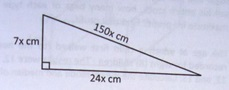
\includegraphics[width=5cm]{./img/quad1.jpg}
	\end{center}
	
	\begin{itemize}
	\item[(i)] Find the value of x
	\item[(ii)] Calculate the area of the triangle
	\end{itemize}		
	
	\item Given the right angled triangle below whose sides are measured in centimeters determine:
		\begin{itemize}
		\item[(i)] The value of x
		\item[(ii)] The area of the triangle
		\end{itemize}
		
		\begin{center}
		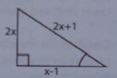
\includegraphics[width=3cm]{./img/quad2.jpg}
		\end{center}
		
	\item Study the following diagram carefully and answer the questions that follow.
	\begin{center}
	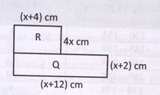
\includegraphics[width=4cm]{./img/quad3.jpg}
	\end{center}	
	
		\begin{itemize}
		\item[(a)]
			\begin{itemize}
			\item[(i)] Write down an expression for the area of rectangle R.
			\item[(ii)] Show that the total area of rectangle R and O is $(5x^2 + 30x + 24)$ cm$^2$.
			\end{itemize}					
		\item[(b)] If the total area of R and Q is 64 cm$^2$, calculate the value of $x$ correct to 1 decimal place.			
		\end{itemize}			

\end{enumerate}
	
	
	
	\subsection{Logarithms}
\begin{enumerate}

	\item Solve $\log_a(x^2 + 3) - \log_ax = 2\log_a2$.
	
	\item Evaluate without using mathematical tables $2\log 5 + \log 36 - \log 9$	
	
	\item Simplify $\cfrac{\log x^4 - \log x}{\log x^3 - \log x}$

	\item Simplify $2\log_{10} 25 - 3\log_{10} 5 + \log_{10} 20$.
	
	\item If $\log_a x = 7$, what is $\log_a \left(\cfrac{1}{x}\right)$?
	
	\item Find the value of the expression $2\log 40 + \log \sqrt{81} - 2\log 12$.
	
	\item Solve for $m$: $\log m = 3\log 6 - \frac{1}{3}\log 125 - 4\log 3 - \log \frac{16}{3}$

	\item Express as a single logarithm the expression $\frac{1}{2}\log_c x - 7\log_c y + \log_c z$.
	
	\item Without using tables, find the value of $3\log_{10} 5 + 5\log_{10} 2 - \frac{1}{2}\log_{10} 16$.
	
	\item Evaluate: $\log_3 9 \times \log_4 \cfrac{1}{64} \times \log_7 \cfrac{1}{7}$
	
	\item Simplify $\log_2 32 - \log_3 9$.
	
	\item It is given that $\log_{10} x + \log_{10} 20 = 2$. Find the value of $x$.
	
	\item Solve the equation $\log_4 5x - \log_4 (x + 2) - \log_4 3 = 0$.
	
	\item Evaluate without using tables $\log_5 \sqrt[3]{605}$
	
	\item If $\cfrac{\log k}{\log 9} = \cfrac{\log 256}{\log 16}$, find the value of $k$.
	
	\item Solve for $x$ in the logarithmic equation $2\log x = \log 4 + \log (2x - 3)$
	
	\item It is given that $n\log_5 125 = \log_2 64$. What is $n$?
	
	\item Find $x$ if $\log_x 32 = 5$.
	
	\item Solve for $x$ if $\log_{10} (x^2 - 3x - 44) = 1$
	
	\item If $\log_4 x = y$, show that $\log_2 x = 2y$. Hence find the value of $x$ given that $\log_2 x + \log_4 x = 9$.
	
	\item Find the value of $a$ if $\log_a 81 - \log_2 32 = -1$.
	
	\item Solve for $x$, given that $\log_3 x - \log_3 (x - 8) = 2$.
	
	\item Without using tables, calculate the value of\\
	(a) $\log_{10}6$	(b) $\log_{10}0.9$\\
	($\log_{10}2 = 0.3010$, $\log_{10}3 = 0.4771$)
	
	\item If $\log 2 = 0.3010$, find the value of $\log 5$.
	
	\item If $\log p = 1.813$ and $\log q = 2.513$, find the value of $pq^2$
	
	\item Using properties of logarithms show that $\log_{10} 15 = 1.17609$ given that $\log_{10} 2 = 0.30103$ and $\log_{10} 3 = 0.47712$.
	
	\item If $\log a = 1.3010$, $\log b = 1.4771$ and $\log c = 1.7782$, calculate $\log \sqrt{\cfrac{a^2b}{c^2}}$ 
	
	\item Evaluate $\log_{10} \cfrac{(0.1575 \times 27500)}{315}$ given that $\log_{10} 1.575 = 0.1973$, $\log_{10} 2.75 = 0.4393$ and $\log_{10} 3.15 = 0.4983$.

	\item Use logarithms to calculate $(3.25)^{10} + \left(\cfrac{40.9}{6.692}\right)^3$\\
	Express your answer in the form $A \times 10^n$, where $1 \leq A < 10$ and $n$ is an integer, to 2 significant figures.
	
	\item By using logarithm tables evaluate: $\sqrt{\cfrac{86.21 \times 2.734}{5.218 \times 0.724}}$
	
	\item Use common logarithm tables to find the value of $\cfrac{2.055 \times 20.35 \times 6.325}{100.5 \times 0.045}$
	
	\item By using logarithm tables evaluate: $\cfrac{88.76 \times 0.0278}{5678 \times 875.8}$

\end{enumerate}


	\subsection{Similarity / Congruence}
\begin{enumerate}

	\item In the figure drawn below find the value of $x$ if $\hat{B} = 37^\circ$.
	
	\begin{center}
	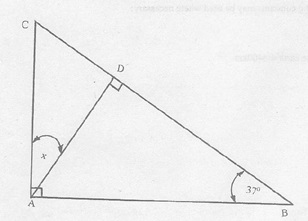
\includegraphics[width=5cm]{./img/sim1.jpg}
	\end{center}
	
	\item In the figure below DE is parallel to BC, AD = 6 cm, BD = 3 cm, DE = 4 cm and $A\hat{B}C = 90^\circ$.
	
	\begin{center}
	\includegraphics[width=3cm]{./img/sim2.jpg}
	\end{center}
	
	Calculate:
	\begin{itemize}
	\item[(i)] the length of BC
	\item[(ii)] the ratio AE\slash AC
	\end{itemize}
	
	\item In $\bigtriangleup ABC$, $M$ is the midpoint of $\overline{AB}$ and $N$ is the midpoint of $\overline{AC}$. Prove that $\overline{MN} \parallel \overline{BC}$ and $\overline{MN} = \frac{1}{2}\overline{BC}$.
	
	\item The ratio of the area of two similar triangles is 1 : 4. Find the ratio of their corresponding sides.
	
	\item If polygons $X$ and $Y$ are similar and their areas are 16 cm$^2$ and 49 cm$^2$ respectively, what is the length of a side of polygon $Y$ if the corresponding side of polygon $X$ is 28 cm?
	
	\item Triangles O and P are similar. A side of triangle O is 8 cm long, while the corresponding side of triangle P is 16 cm long. If the area of triangle O is 40 cm$^2$, what is the area of triangle P?
	
	\item 
		\begin{itemize}
		\item[(i)] Show whether triangles PQR and ABC are similar or not.
	\begin{center}
	\includegraphics[width=7cm]{./img/sim14.jpg}
	\end{center}
		\item[(ii)] Find the relationship between $y$ and $x$ in the triangles given above.
		\end{itemize}
		
	\item In the figure below, SR is parallel to PQ, SX = 3 cm, XQ = 8 cm, PQ = 12 cm and XR = 2.7 cm.
	\begin{center}
	\includegraphics[width=4cm]{./img/sim15.jpg}
	\end{center}
		\begin{itemize}
		\item[(i)] Show that $\bigtriangleup PQX$ and $\bigtriangleup RSX$ are similar.
		\item[(ii)] Calculate the length of SR and PX.
		\end{itemize}
	
	\item With reference to the figure below, calculate the length of segment $\overline{CE}$.
	
	\begin{center}
	\includegraphics[width=5cm]{./img/sim3.jpg}
	\end{center}

		\item In the figure below, calculate the length $\overline{BC}$ if $\overline{AD} = 4$ cm, $\overline{DE} = 3$ cm, $\overline{CE} = 5$ cm and $A\hat{B}C$ and $A\hat{D}E$ are both right angles.
	
	\begin{center}
	\includegraphics[width=4cm]{./img/sim10.jpg}
	\end{center}

	\item In the figure below, BC is parallel to DE, AB = AC and CE = 2.5 cm. DE = 6 cm. The height of trapezium BCED is 1.5 cm.
	
	\begin{center}
	\includegraphics[width=5cm]{./img/sim4.jpg}
	\end{center}

	\begin{itemize}
	\item[(a)] Prove that the triangles ABC and ADE are similar.
	\item[(b)] Calculate the length of AE.
	\end{itemize}
	
	\item In the diagram below, show that $\cfrac{AD}{AB} = \cfrac{CD}{AC}$
	
	\begin{center}
	\includegraphics[width=5cm]{./img/sim7.jpg}
	\end{center}

	\item $\bigtriangleup ABC$ is similar to $\bigtriangleup DEF$. AB = 8 cm while DE = 12 cm. Find the area of $\bigtriangleup ABC$ if that of $\bigtriangleup DEF$ is 45 cm$^2$.
	
	\item In the figure below, $\overline{PQ} \parallel \overline{BC}$, $\overline{AP} = 3$ cm, $\overline{AQ} = 2$ cm and the area of $\bigtriangleup APQ = 8$ cm$^2$.
	\begin{center}
	\includegraphics[width=5cm]{./img/sim8.jpg}
	\end{center}

	\begin{itemize}
	\item[(a)] Show that $\bigtriangleup APQ$ is similar to $\bigtriangleup ABC$
	\item[(b)] Find the area of $\bigtriangleup ABC$
	\item[(c)] Calculate the length of (i) $\overline{PQ}$  \quad (ii) $\overline{QC}$ 
	\item[(d)] Calculate the height $h$.
	\end{itemize}
	
	\item In the figure below, $m(A\hat{B}C) = 90^\circ$. Point D on $\overline{BC}$ is such that $\overline{AD}$ bisects $B\hat{A}C$. If AD = 4 cm and $m(A\hat{D}B) = 60^\circ$, calculate the length of:
		\begin{itemize}
		\item[(a)] $\overline{AB}$
		\item[(b)] $\overline{DC}$
		\end{itemize}
		
	\begin{center}
	\includegraphics[width=6cm]{./img/sim9.jpg}
	\end{center}
	
	\item In the figure below, $\bigtriangleup ABC$ is similar to $\bigtriangleup CTU$, with AB = 3 cm and CT = 2 cm. The area of $\bigtriangleup CTU$ is 6 square cm. Find the area of $\bigtriangleup ABC$.
	
	\begin{center}
	\includegraphics[width=5cm]{./img/sim11.jpg}
	\end{center}
	
	\item PXQ and RXS are straight lines and PR is parallel to SQ. Calculate PX and RX if PR = XQ = 18 cm, XS = 9 cm and SQ = 12 cm.
	
	\begin{center}
	\includegraphics[width=7cm]{./img/sim12.jpg}
	\end{center}	
	
	\item In the figure below, ABCD is a square. If $\overline{AR} = \overline{BR}$ prove that R is the midpoint of $\overline{DC}$.
	
	\begin{center}
	\includegraphics[width=3cm]{./img/sim13.jpg}
	\end{center}	
	
	
%congruency	
	\item ABCD is part of a regular polygon. Show that the triangles ABC and BCD are congruent.
	
	\begin{center}
	\includegraphics[width=5cm]{./img/sim5.jpg}
	\end{center}
	
	\item In the figure below, $\overline{AC} = \overline{CB}$ and $D\hat{A}C$ and $D\hat{B}C$ are right angles. Prove that $\bigtriangleup ACD \equiv \bigtriangleup CBD$.
	
	\begin{center}
	\includegraphics[width=5cm]{./img/sim6.jpg}
	\end{center}
	
\end{enumerate}	

	\subsection{Geometrical Transformations}
	
	See Form IV \nameref{f4trans}.

	\subsection{Pythagoras Theorem}
	
	See \nameref{f2quadeqnsgeo} in Form II \nameref{f2quadeqns} as well as applications in Form IV \nameref{f4trig}.
	
	\subsection{Trigonometry}
	
	See Form IV \nameref{f4trig}.
	
	\subsection{Sets}
\begin{enumerate}

	\item A survey conducted at Omega secondary school showed that 15 students play volleyball, 11 play basketball and 6 play both volleyball and basketball. If everyone plays at least one of these games, find the number of students who play the following games (using a Venn diagram):
		\begin{itemize}
		\item[(a)] volleyball or basketball;
		\item[(b)] basketball but not volleyball;
		\item[(c)] volleyball only.
		\end{itemize}

	\item In a class of 30 students, 17 participate in English debate, 12 participate in English debate and sports. If every student is required to participate in at least one of these two events, find the number of students who participate in:
	\begin{itemize}
	\item[(i)] English debate only
	\item[(ii)] sports only.
	\end{itemize}

	\item In a class of 42 students, 31 students study History and 26 study Physics. Using VVenn diagrams or otherwise, find the number of students who study Physics only.
	
	\item In a certain school there are 50 pupils studying both Basic Mathematics and Additional Mathematics. School regulations require that an Additional Mathematics pupil must come from the Basic Mathematics class. In the school, 10 pupils do not study Basic Mathematics. If only 100 pupils study Basic Mathematics but not Additional Mathematics, how many pupils:
	\begin{itemize}
	\item[(i)] are in the school?
	\item[(ii)] study either Basic Mathematics or Additional Mathematics?
	\item[(iii)] do not study Additional Mathematics?
	\end{itemize}
	\noindent Hint: (Use Venn diagram)
	
	\item There are 60 people at a meeting. 35 are businesspersons, 32 are employees and 15 are both businesspersons and employees.
	\begin{itemize}
	\item[(i)] How many are businesspersons or employees?
	\item[(ii)] How many are neither businesspersons nor employees?
	\end{itemize}
	
	\item There are 30 men at a wedding. Twenty are businessmen, twelve are fishermen and 6 are both businessmen and fishermen.
	\begin{itemize}
	\item[(i)] How many are neither businessmen nor fishermen?
	\item[(ii)] How many are either businessmen or fishermen?
	\end{itemize}
	
	\item 
	\begin{itemize}
	\item[(a)] In a boys' school of 200 students, 90 play football, 70 play basketball and 50 play tennis; 26 play basketball and football, 20 play basketball and tennis, 16 play tennis and football while 10 play all three games. Represent this information in a well labeled Venn diagram.
	\item[(b)] From the information given in (a), how many students in the school do not play:
	\begin{itemize}
	\item[(i)] football
	\item[(ii)] basketball
	\item[(iii)] tennis.
	\end{itemize}
	\end{itemize}
	
	\item Student test results on three subjects; Mathematics, Physics and Chemistry show that 20 passed Chemistry, 5 passed all three subjects, 12 passed Mathematics and Physics and 16 passed Mathematics and Chemistry. Each student passed at least two subjects.
	\begin{itemize}
	\item[(i)] Draw a well labeled Venn diagram to represent these results.
	\item[(ii)] How many students passed Physics and Chemistry?
	\item[(iii)] How many students did the test?
	\end{itemize}

	\item A survey of 240 houses showed that all of them kept a farm or a garden or both. If 180 kept gardens and 79 kept farms, how many houses kept both?
	
	\item In a school of 75 pupils, 45\% of the pupils take Biology but not Chemistry, 32\% take both subjects and 10\% of them take Chemistry but not Biology. How many pupils do not take either Biology or Chemistry?
	
	\item In a Form four class of 24 students, 10 students take basic mathematics only, 12 students take physics and 4 students take both subjects. Using a Venn diagram, find:
	\begin{itemize}
	\item[(i)] The number of students taking physics only.
	\item[(ii)] The number of students taking mathematics.
	\item[(iii)] The number of students who take neither of the two subjects
	\end{itemize}
	
	\item In a class of 36 students, 24 take Chemistry whilst 17 take Physics. What is the least possible number of students who must be taking both Physics and Chemistry?
	
	
%not word problems	
	\item $A$ and $B$ are subsets of the universal set $U$. Find n$(A \cap B)$ given that n$(A) = 39$, n$(A' \cap B') = 4$, n$(B') = 24$ and n$(U) = 65$.

	\item Given $A = \{(x,y):3x + 4y = 10\}$ and $B = \{(x,y):2x - 3y = 1\}$, find $A \cap B$.
	
	\item If $\mu = \{x:1 < x < 11\}$, $A = \{x:2 < x \leq 9\}$, $B = \{x:2 \leq x < 10\}$, list the elements belonging to:
	\begin{itemize}
	\item[(i)] $A \cup B$
	\item[(ii)] $A' \cap B$
	\end{itemize}
	
	\item $P$ and $Q$ are finite sets such that n$(P \cap Q') = 15$, n$(P \cup Q) = 90$ and n$(P \cap Q) = 30$. Without using a Venn diagram, find n$(Q)$.
	
	\item If $A = \{a, b, c\}$, $B = \{b, c, d\}$ and $C = \{c, d, e\}$, show that $A \cup (B \cap C) = (A \cup B) \cap (A \cup C)$.
	
	\item If $\xi = \{a, b, c, d, e\}$, $A = \{a, b, c\}$ and $B = \{e, d\}$, find:
		\begin{itemize}
		\item[(i)] $A' \cap B'$
		\item[(ii)] $(A \cap B)'$
		\end{itemize}
		
	\item If n$(A) = 8$, n$(B) = 12$ and $(A \cap B) = 5$, find n$(A \cup B)$.
		
	\item If $\mu = \{p, q, r, s\}$, If $A = \{p, q, r\}$ and If $B = \{r, s\}$, find $(A' \cap B')$.
		
	\item If $A$ and $B$ are subsets of $S$ where\\
	$S = \{x: x$ is a natural number less than 20$\}$\\
	$A = \{x: x$ is an even number$\}$\\
	$B = \{x: x$ is a multiple of 3$\}$\\
	Find: (a) n$(A \cap B)$ \quad (b) n$(A' \cup B')$
	
	\item If $A$ is the set of prime factors of 42 and $B$ is the set of prime factors of 330, find n$(A \cap B)$.
	
	\item Given sets $A = \{x:-5 \leq x < 2\}$ and $B = \{x:-1 < x < 4\}$, find the value of $A \cap B$.
	
	\item Given $N = \{x:1 \leq x \leq 20\}$. Find the following subsets of $N$:
		\begin{itemize}
		\item[(i)] $A = \{x: x$ is a multiple of 3$\}$
		\item[(ii)] $B = \{x: x$ is a multiple of 4$\}$
		\item[(iii)] $A'$ \quad (iv) $B'$ \quad (v) $(A \cup B)'$ \quad and \quad (vi) $A' \cap B'$.
		\end{itemize}
		
	\item If $A$ and $B$ are any two disjoint sets, show the region represented by $A' \cap B'$ on a Venn diagram.
	
	\item $U = \{10, 20, 30, 40\}$, $A = \{10, 30\}$, $B = \{40, 10\}$, find:
		\begin{itemize}
		\item[(a)]
			\begin{itemize}
			\item[(i)] $A' \cup B'$
			\item[(ii)] $A \cap B'$
			\end{itemize}
		\item[(b)] If $A$ is a subset of $B$, represent the two sets in a Venn diagram.
		\end{itemize}
		
	\item If n$(A \cap B') = 8$, n$(B \cap A') = 5$ and n$(A \cup B) = 20$, 
		\begin{itemize}
		\item[(i)] Display the information in a Venn diagram.
		\item[(ii)] Give the values of n$(A)$ and n$(B)$.
		\end{itemize}
		
	\item Given that $A = \{x:0 \leq x \leq 8\}$ and $B = \{x:3 \leq x \leq 11\}$, where $x$ is an integer, in the same form, present in a Venn diagram:\\
	(i) $A \cup B$ \quad (ii) $A \cap B$\\
	and hence find the elements in each set.
	
	\item If $E = \{$integers between 1 and 11$\}$\\
	$A = \{x:2 < x \leq 9\}$\\
	$B = \{x:1 \leq x < 10\}$
		\begin{itemize}
		\item[(a)] Draw a Venn diagram to illustrate these sets.
		\item[(b)] List the elements belonging to:\\
			(i) $A \cup B$ \quad (ii) $A' \cap B$
		\item[(c)] State n$(A \cap B')$
		\end{itemize}
		
	\item From the figure below, answer the following questions.
	
	\begin{center}
	\includegraphics[width=6cm]{./img/set1.jpg}
	\end{center}
	
	\begin{itemize}
	\item[(a)] List down members of $(P \cup Q)'$
	\item[(b)] Find n$(P \cup Q \cup R)'$
	\item[(c)] Find n$(Q \cup R) - $ n$(P \cap R)$
	\end{itemize}
	
	\item In the Venn diagram below, the number of elements in various regions are as indicated.\\
	If n$(A \cup B \cup C) = 150$, find the value of $x$.
	
	\begin{center}
	\includegraphics[width=7cm]{./img/set2.jpg}
	\end{center}
	
	\item In the figure drawn below, find the number of elements in sets:
		\begin{itemize}
		\item[(a)] $A' \cap (B \cup C)$
		\item[(b)] $(A' \cap B') \cup (B \cup C')$
		\end{itemize}
		
	\begin{center}
	\includegraphics[width=5cm]{./img/set3.jpg}
	\end{center}
	

\end{enumerate}


	\subsection{Statistics}
	
	See Form III \nameref{f3stats}.


\section{Form III}

	\subsection{Relations / Functions}
\begin{enumerate}


			\subsubsection{Graphs, Domain, Range}
%relations

	\item Consider the relation $R = \{(x,y): y = x^2 + 4x\}$
		\begin{itemize}
		\item[(a)] Complete the following table for the relation $R$.\\
		\begin{tabular}{|c|c|c|c|c|c|c|c|c|c|c|} \hline
		$x$ &-6&-5&-4&-3&-2&-1&0&1&2&3 \\ \hline
		$y$ &&&&&&&&&& \\ \hline
		\end{tabular}
		\item[(b)] Plot the graph of the relation $R$.
		\item[(c)] Use the graph to solve the equation $x^2 + 3 = -4x$.
		\end{itemize}
		
	

		
%functions
	\item A function $f$ is defined by $f: \rightarrow 2x^2 - 2x - 1$ where $x$ is the set $\{-2, -1, 0, 1, 2, 3\}$;
		\begin{itemize}
		\item[(a)] Write down the set of ordered pairs $(x, f(x))$.
		\item[(b)] Represent the set of ordered pairs $(x, f(x))$ in a pictorial diagram.
		\item[(c)] Draw the graph of $f(x)$.
		\item[(d)] Find the maximum or minimum value of the function $f(x) = 2x^2 - 2x - 1$.
		\end{itemize}

	\item A function $f$ is defined by the formula $f(x) = \sqrt{x}$, where $x$ is a whole number.
		\begin{itemize}
		\item[(a)] Evaluate $f(9)$
		\item[(b)] If $f(x) = 16$, find the value of $x$.
		\item[(c)] Find the value of $\cfrac{f(200)}{f(2)}$
		\end{itemize}		
		
	\item A function $f$ is defined by: $f(x) = |x - 2|$.
		\begin{itemize}
		\item[(i)] Evaluate $f(-3)$.
		\item[(ii)] Find $x$ if $f(x) = 6$.
		\end{itemize}		 
		
	\item If $f(x) = 5x^2 + 17x - 12$,
		\begin{itemize}
		\item[(a)]
			\begin{itemize}
			\item[(i)] Evaluate $f(10) - f(5)$
			\item[(ii)] Factorize $f(x)$
			\end{itemize}
		\item[(b)] Determine the domain and range of $f(x)$
		\end{itemize}
		
	\item The curve $y = ax^2 + bx + c$ passes through the points (1,8), (0,5) and (3,20). Find the values of $a$, $b$ and $c$ and hence the equation of the curve.
	
	\item If $f(x) = \cfrac{x + 2}{x^2 - x- 6}$, find the values of $x$ for which the function is not defined.
	
	\item The function $f$ is defined by $f: \rightarrow ax + b$, for $x \in R$, where $a$ and $b$ are constants. It is given that $f(2) = 1$ and $f(5) = 7$.
		\begin{itemize}
		\item[(i)] Find the value of $a$ and $b$
		\item[(ii)] Solve the equation $f \circ f(x) = 0$
		\end{itemize}
		
	\item Draw the graph of $x^2 = 2 + y$.
	
	\item It has been specified that $f(x) = 2x^2 - 5x - 3$ ranges from $x = -2$ to $x = 4$.
		\begin{itemize}
		\item[(a)] Draw the graph of $f(x)$.
		\item[(b)] From the graph drawn in (a) above:
			\begin{itemize}
			\item[(i)] find the value of $x$ for which $f(x) = -10$.
			\item[(ii)] determine the line from which the curve is symmetrical.
			\item[(iii)] find the values of $x$ by which $f(x)$ is negative.
			\item[(iv)] solve the equation $2x^2 - 5x - 3 = 0$.
			\end{itemize}
		\end{itemize}

	\item A function is defined by $f(x) = \cfrac{x}{x + 3}$; sketch the graph of $f$.
	
	\item 
		\begin{itemize}
		\item[(a)] On the same set of axes draw the graphs of $f(x) = x^2 - 4x$ and $y = x - 2$.
		\item[(b)] Using the two graphs in (a), estimate the values of $x$ for which $x^2 - 5x + 2 = 0$, correct to 2 significant digits.
		\end{itemize}
		
		\item Without using a table of values, draw the graph of $y = -x^2 + 4x - 5$ and use it to solve the equation $-x^2 + 4x - 5 = -10$.
		
		\item Sketch the graph of the function $f(x) = -1 + |x|$ and find:
			\begin{itemize}
			\item[(i)] the domain and \quad (ii) the range, of $f(x)$.
			\end{itemize}
			
	\item Sketch the graph of the rational function $y = \cfrac{3x - 4}{x - 3}$ and determine its range.
	
	\item 
		\begin{itemize}
		\item[(a)] 
			\begin{itemize}
			\item[(i)] Draw the graphs of the functions $f(x) = x^2 - 4$ and $g(x) = x + 2$ in the same coordinate system.
			\item[(ii)] Shade the region enclosed by the graphs in (i) indicating the intercepts for both graphs.
			\end{itemize}
		\item[(b)] From the graphs in (a) write the coordinates of the points where $f(x) = g(x)$.
		\item[(c)] State the domain and range of $f(x)$.
		\end{itemize}
		
	\item The functions $f$ and $g$ are defined for the domain: $\{2, 3, 4, 5, 6\}$ and the range of $f = \{8, 10, 12, 14, 16\}$ and that of $g = \{8, 6, 4, 2, 0\}$. Find $fg(3)$.
	
	\item Find the domain and range of $f(x) = \sqrt{1 - x^2}$.
	
	\item Find the domain and range of the relation $y = 3x^2 + 2$.
	
	\item Compute the range of the function $f(x) = x^2 - 4x + 3$ for which the domain is $\{-2, -1, 0, 1, 2, 3\}$.
	
	\item Given the rational function $g(x) = \cfrac{mx^2}{x^2 - 3x + 2}$, determine its domain and range.
	
	\item If $f$ is a function such that:\\
	$f(x) =
	\begin{cases}
	\-3 & \text{if } x \leq -1 \\
	1 & \text{if } -1 < x \leq 2 \\
	4 & \text{if } 2 < x
	\end{cases}$
	
	\begin{itemize}
	\item[(a)] determine the domain and range of $f(x)$.
	\item[(b)] draw the graph of $f(x)$.
	\end{itemize}
	
			\subsubsection{Inverse Functions}
%inverses	
	\item Write down the inverse of the function $f(x) = \frac{1}{2}x + 5$.
	
	\item If $f(x) = \frac{1}{2}x + 5$, find $f^{-1}(6)$.
	
	\item A function is defined by $f(x) = x^2 - 2$. Find:
		\begin{itemize}
		\item[(i)] the inverse, $f^{-1}(x)$ of this function.
		\item[(b)] the value of $f^{-1}(-2)$.
		\item[(c)] the domain of $f^{-1}(x)$.
		\end{itemize}
		
	\item Find $g^{-1}(x)$ and hence evaluate $g^{-1}(18)$ given that $g(x) = 2^x + 2$.
	
	\item Find the inverse of the relation $y = \cfrac{4x + 1}{x - 2}$.
	
	\item Find the inverses of the following:
		\begin{itemize}
		\item[(a)] $\{R = (x,y): y = 4x^2\}$
		\item[(b)] $f(x) = 20^x$
		\end{itemize}
		
	\item The functions $f$ and $g$ are defined by: $f(x) = |x|$ and $g(x) = 2 - 3x$.
		\begin{itemize}
		\item[(i)] Evaluate $f(-3)$.
		\item[(ii)] Find $g^{-1}(x)$ and hence evaluate $g^{-1}(8)$.
		\item[(iii)] Draw on the same axes the graphs of $f$ and $g$.
		\end{itemize}

	\item 
		\begin{itemize}
		\item[(a)] If $f(x) = -2x + 3$ find $f^{-1}(3)$.
		\item[(b)] Draw the graph of $f(x) = |x - 1|$ for $-4 \leq x \leq 4$
		\item[(c)] State the domain and range of $f(x) = |x - 1|$.
		\end{itemize}
		
	\item If $f(x) = x^2 - 4x + 3$, find\\
	(i) $f^{-1}(x)$ \quad (ii) the domain and range of $f(x)$
	
	\item A function is defined by $f(x) = x^2 + 6$ and $g(x)$ is another function of $x$ such that\\
	 $g(x) = \cfrac{f(x) - f(4)}{x - 4}$. \\
	Find (i) $g(-4)$ \quad (ii) $g^{-1}(5)$
	
	\item Given that $g(x) = 5 + \cfrac{x}{2}$, find the values of:\\
	(i) $g^{-1}(6)$ \quad (iii) $g^{-1}(-1)$\\
	(ii) $g^{-1}(0)$ \quad (iv) $g^{-1}(a)$
	
			\subsubsection{Maximum, Minimum Values}
%max, min value	
	\item Find the maximum value of the quadratic equation $2 + 30t - 5t^2$.
	
	\item Draw a graph of the function $y = x^2 - 3x + 2$ for the values of $x$ from -2 to 5. From your graph, find:
		\begin{itemize}
		\item[(a)] the range of the function.
		\item[(b)] the minimum value of $y$ and the value of $x$ at which this minimum value occurs.
		\item[(c)] the solution of the equation $x^2 - 3x - 4 = 0$.
		\item[(d)] the solution of the inequality $x^2 - 3x + 2 > 0$.
		\end{itemize}
		


\end{enumerate}	
	
	
	
	
	\subsection{Statistics} \label{f3stats}
\begin{enumerate}

	\item The table below show the distribution of the ages of boys in one class at Shivone secondary school.\\
	\begin{tabular}{|l|c|c|c|c|} \hline
	Age in years & 14 - 16&17 - 19&20 - 22&23 - 25\\ \hline
	Number of boys&27&14&8&7\\ \hline	
	\end{tabular}
		\begin{itemize}
		\item[(a)] Draw a cumulative frequency polygon for this information.
		\item[(b)] What is the mean age of the class?
		\item[(c)] State the median class.
		\item[(d)] Find the probability that a boy chosen at random from the class has age between 17 - 19 or 23 - 25.
		\end{itemize}

	\item In a survey of the number of children in 12 houses, the following data resulted: 1, 2, 3, 4, 2, 2, 1, 3, 4, 3, 5, 3.
		\begin{itemize}
		\item[(a)] Show this data in a frequency distribution table.
		\item[(b)] Draw a histogram and a frequency polygon to represent this data.
		\item[(c)] Calculate the mean and mode number of children per house.
		\end{itemize}

	\item The following is a record of marks by a group of students in an examination.\\
	
	\begin{tabular}{cccccccccc}
	23&63&82&71&12&63&38&17&23&44 \\
	54&19&70&45&70&43&18&03&02&64 \\
	45&42&40&70&63&28&18&27&58&53 \\
	23&81&70&58&31&83&19&43&72&71 \\
	48&63&62&44&38&37&46&81&73&38 	
	\end{tabular}
	
	\begin{itemize}
	\item[(a)] Tabulate as a frequency distribution using intervals 0 - 9, 10 - 19, etc.
	\item[(b)] Find the class which contains the median.
	\item[(c)] Find the modal class.
	\item[(d)] Calculate the mean mark using the grouped data.
	\end{itemize}
	
	\item The following frequency distribution table shows the monthly salaries for 33 workers in a certain company.\\
	
	\begin{tabular}{|p{2.5cm}|c|c|c|c|c|} \hline
	\textbf{Salary (Tsh)}&20000 - 29000&30000 - 39000&40000 - 49000&50000 - 59000&60000 - 69000 \\ \hline
	\textbf{Number of Workers}&1&4&6&10&8 \\\hline
	\end{tabular}

	\begin{tabular}{|p{2.5cm}|c|c|} \hline
	\textbf{Salary (Tsh)}&70000 - 79000&80000 - 89000 \\ \hline
	\textbf{Number of Workers}&2&2 \\\hline
	\end{tabular}
	
	\begin{itemize}
	\item[(a)] By making the class mark of the class interval 50000 - 59000 as the assumed mean, calculate the mean salary.
	\item[(b)] What is the mode for this distribution?
	\item[(c)] Calculate the median.
	\item[(d)] Find the number of workers whose salaries exceed Tsh 69,500/=.
	\end{itemize}
	
	\item The following table gives the scores of sixty students in a Basic Mathematics test.\\
	
	\begin{tabular}{|c|c|} \hline
	Scores&Frequency \\ \hline
	0 - 10&5 \\ \hline
	10 - 20&7 \\ \hline
	20 - 30&15 \\ \hline
	30 - 40&25 \\ \hline
	40 - 50&8 \\ \hline
	\end{tabular}
	
	Calculate:
	\begin{itemize}
	\item[(a)] The mean score if the assumed mean is obtained from the mid mark of the modal class.
	\item[(b)] The median.
	\item[(c)] The range.
	\end{itemize}
	
	\item Carefully study the frequency distribution table which shows marks for 40 students in a mathematics examination.\\
	
	\begin{tabular}{|l|c|c|c|c|c|} \hline
	Marks & 1 - 20&21 - 40&41 - 60&61 - 80&81 - 100\\ \hline
	Number of Students&3&11&12&8&6\\ \hline	
	\end{tabular}
	
	\begin{itemize}
	\item[(i)] Calculate the mean score, given the assumed mean 50.5.
	\item[(ii)] Determine the modal class.
	\item[(iii)] Draw a cumulative frequency curve and use it to estimate the median.
	\end{itemize}
	
	\item A survey of 50 families showed the number of children per family as follows.\\
	
	\begin{tabular}{|l|c|c|c|c|c|} \hline
	Number of children&1&2&3&4&5 \\ \hline
	Number of families&19&18&9&3&1 \\ \hline	
	\end{tabular}
	
	\begin{itemize}
	\item[(i)] Write down the modal number of children per family.
	\item[(ii)] Find the median number of children per family.
	\item[(iii)] Calculate the mean number of children per family.
	\end{itemize}
	
	\item The age at which a child first walked (to the nearest month) was recorded for eight (8) children. The results were 12, 10, 16, 19, 10, 12, 12 and 13. Calculate the mean, mode and median of the data.
	
	\item A random sample of 100 students was chosen from a school. Each student's blood pressure was measured to the nearest milimetres of mercury as shown in the table below.\\
	
	\begin{tabular}{|l|c|c|c|c|c|c|c|} \hline
	Blood pressure (mmHg)&55 - 59&60 - 64&65 - 69&70 - 74&75 - 79&80 - 84&85 - 89 \\ \hline
	Number of students&1&3&8&17&30&25&16 \\ \hline
	\end{tabular}
	
	\begin{itemize}
	\item[(a)] Calculate the mean and mode of blood pressure.
	\item[(b)] Construct a cumulative frequency table and draw the ogive. From the ogive estimate
		\begin{itemize}
		\item[(i)] the median blood pressure
		\item[(ii)] the percentage of students with blood pressure between 67 mmHg and 76 mmHg.
		\end{itemize}
	\end{itemize}
	
	\item Carefully study the frequency distribution table for the scores of 68 students (in percentage) given here under.\\
	
	\begin{tabular}{|p{3cm}|c|c|c|c|c|c|c|} \hline
	Class Boundary (in percentage)&30 - 39&40 - 49&50 - 59&60 - 69&70 - 79&80 - 89&90 - 99 \\ \hline	
	Frequency&6&12&14&16&8&6&6 \\ \hline
	\end{tabular}
	
	\begin{itemize}
	\item[(a)] Determine the mode of the scores.
	\item[(b)] Calculate the median of the scores.
	\item[(c)] A student is chosen at random from the frequency distribution table above. What is the probability that his score is below 60\%?
	\end{itemize}
	
	\item A survey was made on the number of the people attending conferences on one particular week. A random sample of 100 conference centres was taken and the results were as follows:\\
	
	\begin{tabular}{|c|c|} \hline
	\textbf{Number of people}& \textbf{Number of}\\ 	\textbf{attending conference}&\textbf{conference centres} \\ \hline
	150 - 154&8 \\ \hline
	155 - 159&16 \\ \hline
	160 - 164&43 \\ \hline
	165 - 169&29 \\ \hline
	170 - 174&4 \\ \hline	
	\end{tabular}
	
	\begin{itemize}
	\item[(i)] Draw a histogram and a cumulative frequency curve to represent these results.
	\item[(ii)] Estimate the median of this data from the cumulative frequency curve in (i) above.
	\end{itemize}
	
	\item The pie chart below shows the number of students in one examination centre in different subjects sat for the national examinations.
	
	\begin{center}
	\includegraphics[width=5cm]{./img/stats1.jpg}
	\end{center}
%	\includegraphics[width=5cm]{./img/set3.jpg}
%	\end{center}	
	
	Given that 220 candidates did History, find:
	\begin{itemize}
	\item[(i)] The total number of candidates at this examination centre.
	\item[(ii)] The number of students who sat for Civics examination.
	\end{itemize}
	
	\item The following represents age distribution of members of a school choir.\\
	
	\begin{tabular}{|l|c|c|c|c|c|c|} \hline
	Age&14&15&16&17&18&19 \\ \hline
	Frequency&2&1&3&6&5&3 \\ \hline	
	\end{tabular}
	
	\begin{itemize}
	\item[(a)] How many students are in the school class?
	\item[(b)] What is the modal age?
	\item[(c)] Calculate the mean age of the members of the school choir.
	\item[(d)] What is the probability that a member chosen at random from the choir is
		\begin{itemize}
		\item[(i)] 17 years old?
		\item[(ii)] over or equal to 17 years?
		\end{itemize}
	\item[(e)] Draw a pie chart to show the age distribution of the members of the school choir.
	\end{itemize}
	
	\item The data below represent masses in kg of 36 men:\\
	51; 61; 60; 70; 75; 71; 75; 70; 74; 73; 72; 82; 70; 71; 76; 74; 50; 68; 68; 66; 65; 72; 69; 64; 83; 63; 83; 58; 80; 90; 50; 89; 55; 62; 62; 61.
	\begin{itemize}
	\item[(i)] Prepare a frequency distribution table of class interval of size 5 beginning with the number 50 taking into consideration that both the lower limit and upper class limit are inclusive.
	\item[(ii)] Calculate the mean and mode from the frequency distribution table prepared in (i) above by using assumed mean from the class mark of the modal class.
	\end{itemize}
	
	\item The data below shows test scores of a certain class in mathematics.
	
	\begin{tabular}{cccccccccc}
	21&21&21&22&22&22&22&23&23&24 \\
	24&24&21&24&24&25&26&27&27&27 \\
	\end{tabular}
	
	Construct a frequency distribution table showing scores $x$ and frequency $f$.
	
	\item Carefully study the frequency distribution table which shows marks for 40 students in a mathematics examination.\\
	
	\begin{tabular}{|l|c|c|c|c|c|} \hline
	Marks & 1 - 20&21 - 40&41 - 60&61 - 80&81 - 100\\ \hline
	Number of Students&3&11&12&8&6\\ \hline	
	\end{tabular}
	Determine:
	\begin{itemize}
	\item[(i)] The mean, given the assumed mean is 50.5
	\item[(ii)] The median
	\item[(iii)] Modal class and its corresponding class mark.
	\end{itemize} 
	
	\item The table shows the masses of 100 students to the nearest kilogram.\\
	
	\begin{tabular}{|l|c|c|c|c|c|} \hline
	Mass (kg) &60 - 62&63 - 65&66 - 68&69 - 71&72 - 74 \\ \hline
	Frequency&5&18&42&27&8 \\ \hline	
	\end{tabular}
	
	\begin{itemize}
	\item[(a)] Determine the mean of the masses.
	\item[(b)] Find the mode.
	\item[(c)] Draw a cumulative frequency curve and use it to determine the median of the masses.
	\end{itemize}
	
	\item The table below shows the distribution of 100 shops and their profit per shop recorded in a certain month.\\
	
	\begin{tabular}{|l|c|c|c|c|c|c|} \hline
	Profit per shop in thousands of shs.&30 - 34&35 - 39&40 - 44&45 - 49&50 - 54&55 - 59 \\ \hline
	Number of shops&12&18&C&C - 7&C - 10&6 \\ \hline	
	\end{tabular}
	
	\begin{itemize}
	\item[(a)] Find the value of C.
	\item[(b)] Prepare the frequency distribution and use it to determine the modal class.
	\item[(c)] Draw a histogram and frequency polygon on the same diagram.
	\end{itemize}
	
	\item The frequency distribution of the length of a sample of 100 nails, measured to the nearest mm, is shown below.\\
	
	\begin{tabular}{|l|c|c|c|c|c|c|c|} \hline
	Length&40 - 42&43 - 45&46 - 48&49 - 51&52 - 54&55 - 57&58 - 60 \\ \hline
	Frequency&4&9&13&20&34&18&2 \\ \hline	
	\end{tabular}
	
	\begin{itemize}
	\item[(a)] How many nails have length less than 51.5 mm?
	\item[(b)] Calculate the mean length.
	\item[(c)] Draw a histogram and use it to estimate the modal length.
	\item[(d)] State the modal class.
	\end{itemize} 
	
	\item The daily wages of one hundred men are distributed as shown below:\\
	
	\begin{tabular}{|p{4cm}|c|c|c|c|} \hline
	Wage in Tshs $\times$ 1000&3.0 - 3.4&3.5 - 3.9&4.0 - 4.4&4.5 - 4.9 \\ \hline
	Number of men&4&6&10&14 \\ \hline	
	\end{tabular}
	
	\begin{tabular}{p{4cm}|c|c|c|c|} \cline{2-5}
	&5.0 - 5.4&5.5 - 5.9&6.0 - 6.4&6.5 - 6.9 \\ \cline{2-5}
	&x&20&14&6 \\ \cline{2-5}	
	\end{tabular}
	
	\begin{itemize}
	\item[(a)] Find x.
	\item[(b)] Calculate the daily mean wage of the 100 men.
	\item[(c)] Draw a histogram to represent this data.
	\end{itemize}
	
	\item The table below shows the distribution of scores of 46 students in a mathematics examination.\\
	
	\begin{tabular}{|l|c|c|c|c|c|} \hline
	Marks in \%&35 - 45&46 - 56&57 - 67&68 - 78&79 - 89 \\ \hline
	No. of students&20&12&7&6&1 \\ \hline	
	\end{tabular}
	
	\begin{itemize}
	\item[(a)] 
		\begin{itemize}
		\item[(i)] Calculate the mean score.
		\item[(ii)] What is the modal class?
		\end{itemize}		 
	\item[(b)] Draw a cumulative frequency curve and estimate from  it the median score.
	\end{itemize} 
	
	\item The heights in centimetres of 100 students of a certain school were recorded as follows:\\
	
	\begin{tabular}{|l|c|c|c|c|c|c|c|c|c|} \hline
	Height in cm&150&155&160&165&170&175&180&185&190 \\ \hline
	Frequency&4&9&12&16&25&20&8&4&2 \\ \hline	
	\end{tabular}
	
	From the above information answer the following questions:
	\begin{itemize}
	\item[(a)] Draw a frequency polygon.
	\item[(b)] Determine the mean, median and mode.
	\item[(c)] Compute the variance and standard deviation.
	\item[(d)] A student is chosen at random from this school. What is the probability that his height is greater than 160 cm?
	\end{itemize} 
	
	\item The following table shows the grade points scored by 50 students in a Mathematics test.\\
	
	\begin{tabular}{|l|c|c|c|c|c|c|} \hline
	Grade points&0&1&2&3&4&5 \\ \hline
	Frequency&1&12&14&15&7&1 \\ \hline	
	\end{tabular}
	
	\begin{itemize}
	\item[(i)] Represent this information by a frequency polygon. 
	\item[(ii)] Find the mode and median.
	\item[(iii)] Find the probability that, if a student is chosen at random, then her grade point score will be greater than or equal to 3.
	\end{itemize} 
	
	\item The examination results (rounded to the nearest whole number \%) are given for a group of students.\\
	
	\begin{tabular}{|l|c|c|c|c|c|} \hline
	Mark (\%)&30 - 39&40 - 49&50 - 59&60 - 69&70 - 79 \\ \hline
	Frequency &5&3&20&2&10 \\ \hline	
	\end{tabular}
	
	\begin{itemize}
	\item[(a)] State the modal class.
	\item[(b)] Estimate the mean score.
	\item[(c)] Estimate the median score.
	\item[(d)] Estimate the mode.
	\end{itemize} 
	
	\item The scores of a Physics test taken by 60 students were recorded as follows:\\
	
	\begin{tabular}{ccccccccccccc}
	30&56&21&49&34&58&22&38&27&31&35&41&53 \\
	25&34&48&33&58&20&34&30&50&26&52&32&63 \\
	25&50&36&29&34&21&61&33&51&20&41&30&57 \\
	26&28&45&36&59&26&60&42&21&63&56&36&54 \\
	43&24&30&27&26&56&35&32&&&&& \\	
	\end{tabular}
	
	\begin{itemize}
	\item[(a)] Arrange these scores into grouped frequency distribution table starting with the classes 20 - 24, 25 - 29, 30 - 34, $\ldots$
	\item[(b)] Calculate the mean score.
	\item[(c)] Draw the histogram and use it to estimate the mode.
	\item[(d)] Draw the ogive and use it to estimate the median.
	\end{itemize}
	
	\item Florina sat for ten examinations. In the first six subjects she scored an average of 65 marks while in the last four subjects she scored an average of 60 marks. Find the average score for all the ten examinations.
	
	\item The mean of $n$ numbers is 20. If the same numbers together with 30 give a new mean of 22, find $n$.
	
	\item Find the geometric mean and arithmetic mean of 18 and 72.
	
	\item Calculate the geometric mean and arithmetic mean of $3 + \sqrt{5}$ and $3 - \sqrt{5}$.
	
	\item The arithmetic mean and geometric mean of two numbers $m$ and $n$ are 17 and 15 respectively. Find the two numbers.
	

\end{enumerate}	
	
	
	
	\subsection{Rates and Variations}
\begin{enumerate}

		\subsubsection{Variations}
%variations
	\item If $y$ is directly proportional to $x$, find the value of each of $a$, $b$ and $c$ in the table below.\\
	\begin{tabular}{|c|c|c|c|c|} \hline
	$y$ & 8 & 12 & $b$ & 32 \\ \hline
	$x$ & 2 & $a$ & 6 & $c$ \\ \hline
	\end{tabular}

	\item $x$ is directly proportional to $y^2$ and inversely proportional to $z$. If $x = 10$ when $y = 2$ and $z = 2$, find $x$ when $y = 6$ and $z = 9$.
	
	\item Given that $p$ varies directly proportional to $q$ but inversely proportional to $r$ and that, when $p = 35$, $q = 7$ and $r = 6$. Find the value of $p$ when $q = 2$ and $r =5$.
	
	\item Given that $y$ is inversely proportional to $x$ and that when $x$ is 6, $y = 8$, find the value of $y$ when $x = 4$.
	
	\item Given that $y$ varies inversely as $x^2$ and that $y = 4$ when $x = 3$, calculate the value of $y$ when $x = 6$.
	
	\item $y$ is inversely proportional to $x$. When $x = 3$, $y = 2$. Find the value of $y$ when $x = \cfrac{1}{3}$.
	
	\item Given that $y$ varies inversely as the square root of $x$ and $y = 2$ when $x = 25$, find the value of $x$ when $y = 4$.
	
	\item If $V$ varies inversely with $n$ and $V = 220$ when $n = 6$, find $V$ when $n = 8$.
	
	\item The number of workers needed to repair a road is inversely proportional to the time taken. If 12 workers can finish the repair in 10 days, how long will 30 workers take?
	
	\item the power ($P$) used in an electric circuit is directly proportional to the square of the current ($I$). When the current is 8 Amperes ($A$), the power used is 640 Watts ($W$).
		\begin{itemize}
		\item[(i)] Write down the equation relating the power ($P$) and the current ($I$);
		\item[(ii)] Calculate the current $I$ when the circuit uses 360 Watts.
		\end{itemize}
	
	\item The surface area of a sphere $V$ mm$^2$ varies directly as the square of its diameter $d$ mm. If the surface area is to be doubled, what ratio must the diameter be altered?
	
	\item The number of eggs which a goose lays in a week varies as the cube root of the average number of hours of sleep she has. When she has 8 hours sleep, she lays 4 eggs. How long does she sleep when she lays 5 eggs?
	
	\item The value $V$ of diamond is proportional to the square of its weight $W$. It is known that a diamond weighing 10 grams is worth shs. 200,000/=.
		\begin{itemize}
		
	\item[(a)] Write down an expression which relates $V$ and $W$.
	\item[(b)] Find the value of a diamond weighing 30 grams.
	\item[(c)] Find the weight of the diamond worth 5,000,000/=.
		\end{itemize}
		
	\item The number of square tiles needed to surface the floor of a hall varies inversely as the square of the length of a side of the tile used. If 2016 tiles of side 0.4 m would be needed to surface the floor of a certain hall, how many tiles of side 0.3 m would be required?
	
	\item Two quantities $P$ and $Q$ are connected by a linear relation of the form $P = KQ + C$, where $K$ and $C$ are constants. Find the equation connecting $P$ and $Q$ if $Q = 60$ when $P = 10$ and $Q = 240$ when $P = 100$ and hence find the value of $K$ and $C$.
	
	\item A variable $a$ varies directly as $b$ and inversely as the square root of $c$. If $a = 0.2$ when $b = 4$ and $c = 100$, find the value of $a$ when $b = 16$ and $c = 64$.
	
	\item The distance of the horizon $d$ km varies as the square root of the height $h$ m of the observer above sea level. An observer at a height of 100 m above sea level sees the horizon at a distance of 35.7 km. Find:
		\begin{itemize}
		
	\item[(i)] The distance of the horizon from an observer 70 m above sea level.
	\item[(ii)] An equation connecting $d$ and $h$.	\end{itemize}
	
	\item The length of the shadow reduces at equal rate as time goes and the sun moves from East to West. If the rate is 2 m to every 3 hrs, at what time will the shadow be, if at 7:00 am the shadow was 8 m long?
	
	\item If $y$ varies inversely as $\sqrt{x}$, and $x$ is multiplied by $n$, what is the ratio of the first $y$ to the second $y$?

		\subsubsection{Rates}
%rates	
	
	\item Taps A and B can fill a tank in 6 and 10 minutes respectively. How long will it take for both taps working together to fill the tank?
	
	\item Three classes working 8 hours a day take 5 days to harvest maize from a school shamba. How long will it take if they were only two classes, but working for 10 hours a day?
	
	\item Sixty people working 8 hours a day take 4 days to cultivate a village farm. How long will it take twenty people to cultivate the same farm if they work 15 hours a day?
	
	\item If six people were to work on the farm, they would finish the work in 10 days. How many more people must be employed in order to finish the work in four days?
	
	\item A radio is sold at Tshs. 40,500/=. This price includes 20\% Value Added Tax (V.A.T.). Calculate the amount of V.A.T.
	
	\item The price of a TV set which includes V.A.T. is shs 133,800.00. If the rate of V.A.T. is 30\%, find the price of the TV before V.A.T. was added.
	
	\item A settlement has a population of 1000 people. Each year 5\% of the people leave the settlement. How many people will remain after 4 years?
	
	\item In a certain bacteria colony there are 100 bacteria and each breaks into two after each hour. Find after how many hours will the size of the colony be 7500?
	
	\item Water flow through a circular pipe of internal radius of 10 cm at 5 m\slash s. If the pipe is always half full, find the number of cubic metres discharged in half an hour. ($\pi = 3.142$)
	
	\item Juma bought motor vehicle spare parts from Japan worth 5,900,000 japanese Yen. When he arrived in Tanzania he was charged custom duty of 25\% on the spare parts. If the exchange rate were as follows:\\
	1 US dollar = 118 Japanese Yen.\\
	1 US dollar = 76 Tanzania Shillings\\
	Calculate the duty he paid in Tanzania Shillings.



\end{enumerate}	
	
	

	\subsection{Sequences and Series}
	
\begin{enumerate}


%sequences
		\subsubsection{Sequences}
		
	\item Write down the next two terms in the following sequence: $\frac{1}{2}, \frac{2}{3}, \frac{3}{5}, \frac{5}{8}, \frac{8}{13}, \ldots$
	
	\item Write down the general term (n\textsuperscript{th} term) of the sequence $\frac{1}{2}, \frac{2}{3}, \frac{3}{4}, \ldots$ Hence find the 60\textsuperscript{th} term.
	
	\item The n\textsuperscript{th} term of a certain sequence is $\frac{5}{2}$n - 1. Find the sum of the first five terms of the corresponding series.
	
	\item Find general term and hence the 30\textsuperscript{th} term of the sequence 1, -2, 4, -8, $\ldots$
	
	
%AP only	

		\subsubsection{Arithmetic Progressions}
		
	\item Show that the numbers between 5 and 250 which are exactly divisible by 4, form an arithmetic progression and hence find the sum of all the numbers.
	
	\item If the 5\textsuperscript{th} term of an arithmetic progression is 23 and the 12\textsuperscript{th} term is 37, find the first term and the common difference.
	
	\item Compute the sum of the first ten terms of the series 1 + 5 + 9 + $\ldots$
	
	\item Given the series 100 + 92 + 84 + $\ldots$ Find:
		\begin{itemize}
		\item[(i)] The 20\textsuperscript{th} term
		\item[(ii)] The sum of the first 20 terms
		\end{itemize}
		
	\item The second term of an A.P. is 2 and the sixth term is -14. What is the
	\begin{itemize}
	\item[(i)] first term
	\item[(ii)] common difference?
	\end{itemize}
	
		
	\item The 5\textsuperscript{th} term of an arithmetic progression is 23 and the 12\textsuperscript{th} term is 37. Find:
	\begin{itemize}
	\item[(i)] the eleventh term
	\item[(ii)] the sum of the first eleven terms by using the values computed in (i) above without using the common difference for this progression.
	\end{itemize}
	
	\item The first four terms of an AP are 2, (a-b), (2a + b + 7) and (a-3b) respectively where a and b are constants.
	\begin{itemize}
	\item[(i)] Find the values of the constants a and b.
	\item[(ii)] The sum of the first 10 terms.
	\end{itemize}
	
	\item If the first term of an arithmetical progression is 3 and the third term is 13, find the second term, the fourth term and the sum of the first ten terms.
	
	\item In an arithmetical progression, the thirteenth term is 27, and the seventh term is three times the second term. Determine the sum of the first ten terms.
	
	\item 
	\begin{itemize}
	\item[(a)] The n\textsuperscript{th} term of an AP is 12 - 4n. Find the first term and the common difference.
	\item[(b)] In an AP the 1\textsuperscript{st} term is -10 the 15\textsuperscript{th} term is 11 and the last term is 41. Find the sum of all terms in the progression.
	\end{itemize}
	
	\item The sum of the first six terms of an AP is 72 and the second term is seven times the fifth term.
	\begin{itemize}
	\item[(i)] Find the first term and the common difference.
	\item[(ii)] Find the sum of the first ten terms.
	\end{itemize}
	
	\item The sum of the first n terms of an arithmetic progression is 2n. If the sum of the first 2n terms of this AP is 3n, what will be the sum of the first 3n terms of the AP?
	
	
	
	
	
%GP only	

			\subsubsection{Geometric Progressions}
			
	\item Find the value of $t$ for which $t - 6$, $2t$ and $8t + 20$ are the first three consecutive terms of a geometric progression.
	
	\item Find the sum of the first four terms of a geometric progression which has a first term of 1 and a common ratio of $\cfrac{1}{4}$.
	
	\item If the third term of a geometric progression is 100 and the sixth term is 800, find the fifth term and the sum of the first two terms.
	
	\item Find the number of terms in the geometric progression: 81 + 27 + 9 + $\ldots$ + $\frac{1}{27}$.
	
	\item The common ratio of a geometrical progression is 2 and the sum of the first eight terms is 1020. Find the first term of the progression.
	
	\item A certain geometric progression has a common ratio of 2 and the sum of the first five terms is 155. Find the first term and give the formula for the n\textsuperscript{th} term.

	\item If 5, x, y and 40 are in geometrical progression, find x and y.
	
	\item In a geometric progression (GP) the sum of the second and third term is 6, and the sum of the third and fourth terms is -12. Find the sum of the first 5 terms of the GP.
	
	\item The 5\textsuperscript{th} term of a GP is 8, the third term is 4 and the sum of the first ten terms is positive. Find the first term, the common ratio and the sum of the first ten terms.
	
	\item Find the k\textsuperscript{th} term of the series
	\begin{center}
	$10 + 5 + \frac{5}{2} + \frac{5}{4} + \frac{5}{8} + \ldots$, where k = 1, 2, 3, $\ldots$
	\end{center}
	
	\item The sum of the first two terms of a geometrical progression is 10 and the sum of the first four terms is 40. Given that all terms of the progression are positive, show that:
	\begin{itemize}
	\item[(i)] the common ratio is $\sqrt{3}$.
	\item[(ii)] the sum of the first n terms is 5(3\textsuperscript{n/2} - 1).
	\end{itemize}

	\item If the sum of n terms of a GP having first term 1 and common ratio $\frac{1}{2}$ is $\frac{31}{16}$, find the number of terms.
	
	\item Find the difference between the sums of the first ten terms of the geometric progressions whose first terms are 7 and 9 and common ratios are 3 and 2 respectively.
	
%ap/geo linked	
			\subsubsection{AP / GP Combined}
			
	\item The fourth, fifth and sixth terms of the series are: (2x + 10), (4x - 4) and (8x + 40) respectively. Calculate the values of x and find the sum of the first ten terms when the series is:
	\begin{itemize}
	\item[(i)] an arithmetic progression
	\item[(ii)] a geometric progression
	\end{itemize}		

	\item The second, fifth and eleventh terms of an arithmetical progression are in geometrical progression, and the seventh term is 4. Find:
	\begin{itemize}
	\item[(a)] the common ratio of the geometrical progression.
	\item[(b)] the common difference of the arithmetical progression.
	\end{itemize}
	
	\item The 4\textsuperscript{th}, 6\textsuperscript{th} and 9\textsuperscript{th} terms of an arithmetical progression (A.P.) forms the first three terms of a geometric progression. If the first term of the A.P. is 3, determine the
	\begin{itemize}
	\item[(a)] common difference of the arithmetical progression.
	\item[(b)] common ratio of the geometrical progression.
	\end{itemize}
	
	\item The second, fifth and seventh terms of an arithmetic progression form three consecutive terms of a geometrical progression. Find the common ratio of the geometrical progression.
	
	\item The second and third terms of an arithmetic progression (AP) are 20 and 22 respectively. Its first, fourth and eighth terms form the first three terms of a geometric progression (GP). Determine:
	\begin{itemize}
	\item[(i)] The common ratio of the geometric progression
	\item[(ii)] The sum of the first four terms of the GP
	\item[(iii)] The tenth term of the AP
	\end{itemize}
	
	\item The second, fourth and eighth terms of an arithmetic progression form three consecutive terms of a geometric progression. If the sum of the third and fifth terms of the geometric progression is 20, find the sum of the first ten terms of the geometric progression.
	
	\item If the 2\textsuperscript{nd}, 4\textsuperscript{th} and 7\textsuperscript{th} terms of an AP are the first consecutive terms of the GP, find:
	\begin{itemize}
	\item[(a)] The common ratio
	\item[(b)] The sum  of the first 4 terms of the AP if the first term is 12.
	\end{itemize}
	
%compound interest	
			\subsubsection{Interest}
			
	\item The amount obtained after investing a principal P for 3 years was shs. 2519.40. If the amount was compounded annually at a rate of 8\%, fiind the value of P.
	
	\item John wants to invest a certain sum of money so that its value after 3 years will be sh. 100,000/=. How much should he invest at 5\% p.a. compound interest?

	\item How long would it take a sum of money to double itself at 5\% per annum compound interest?
	
	\item If sh. $P$ is invested at $r$\% compound interest, it amounts to sh. $A$ after $n$ years, where:
	\begin{center}
	$A = P(1 + \frac{r}{100})^n$
	\end{center}
	\noindent Find $A$, if $P$ = 250, $r$ = 4, and $n$ = 12.
	
	\item A small business sells products worth 1,000,000 Tshs during its first year. The owner of the business has set a goal of increasing annual sales by 750,000 Tshs each year. Assuming this goal is met, find the total sales during the first 10 years of the business in operation.
	
	
	
	
\end{enumerate}
	
	
	
	\subsection{Circles}
\begin{enumerate}
	\item Given two circles having radius 14 cm and 7 cm,
		\begin{itemize}
		\item[(i)] find their corresponding area.
		\item[(ii)] verify that the ratio of the areas of any two circles equals the square of the ratio of their radii $\left(\text{use }\pi = \cfrac{22}{7}\right)$.
		\end{itemize}
		
	\item AOP is the diameter of a circle with centre 0.\\
	Given that ABC is a straight line and angle $Q\hat{B}C = 81^\circ$, calculate the value of angle $P\hat{A}Q$.
	\begin{center}
	\includegraphics[width=5cm]{./img/circ1.jpg}
	\end{center}	
	
	\item The chords AB and CD of the circle given below meet at point O inside the circle. Given that AO = 8 cm, OC = 9 cm and OD = 4 cm, find OB.
	\begin{center}
	\includegraphics[width=5cm]{./img/circ19.jpg}
	\end{center}		

	\item In the figure below, O is the centre of the circle. Find the value of $x$.
	\begin{center}
	\includegraphics[width=5cm]{./img/circ2.jpg}
	\end{center}

	\item In the figure below ACD is an equilateral triangle and ABCD is a cyclic quadrilateral. Given that $E\hat{C}D = 20^\circ$, find the size of angle $E\hat{B}C$.
	\begin{center}
	\includegraphics[width=5cm]{./img/circ3.jpg}
	\end{center}

	\item In the circle ABCD below, AB is an arc of $43^\circ$ and CD is an arc of $25^\circ$. O is the centre of the circle. What is the degree measure of $D\hat{L}C$?
	\begin{center}
	\includegraphics[width=5cm]{./img/circ4.jpg}
	\end{center}

	\item In the figure drawn here under, $\overline{AB} = 156$ mm, $\overline{CD} = 96$ mm and $\overline{PA}$ is 12 mm shorter than $\overline{PD}$. Find the length of $\overline{PA}$.
	\begin{center}
	\includegraphics[width=5cm]{./img/circ5.jpg}
	\end{center}

	\item In the figure below, O is the centre of the circle, $A\hat{O}B = 120^\circ$ and $C\hat{D}B = 15^\circ$. Find the value of $x$.
	\begin{center}
	\includegraphics[width=6cm]{./img/circ6.jpg}
	\end{center}

	\item Determine the value of $x$ in the figure below where O is the centre of the circle.
	\begin{center}
	\includegraphics[width=5cm]{./img/circ7.jpg}
	\end{center}

	\item If, in the diagram below, ABCD is a cyclic quadrilateral, O is the centre and m$(A\hat{D}C) = 140^\circ$, find:\\
	(a) m$(A\hat{B}C)$ \quad (b) m$(A\hat{O}C)$ \quad (c) m$(O\hat{A}C)$
	\begin{center}
	\includegraphics[width=5cm]{./img/circ8.jpg}
	\end{center}

	\item In the diagram below, $\overline{DC}$ is a diameter of the circle with centre O. The chord $\overline{AB}$ is parallel to $\overline{DC}$. Find the value of $x$ given that m$(A\hat{O}D) = 70^\circ$.
	\begin{center}
	\includegraphics[width=5cm]{./img/circ9.jpg}
	\end{center}

	\item In the figure below find $x$.
	\begin{center}
	\includegraphics[width=5cm]{./img/circ10.jpg}
	\end{center}

	\item In the figure shown below, O is the centre of the circle, $A\hat{O}D = 100^\circ$ and $C\hat{D}B = 40^\circ$. Find the value of $x$ if AC is a line segment.
	\begin{center}
	\includegraphics[width=6cm]{./img/circ11.jpg}
	\end{center}

	\item In the figure below, $\overline{AT}$ is the diameter of the circle. Points $A$, $B$ and $P$ lie on a straight line. $\overline{PT}$ is a tangent to the circle at $T$. If $AP = x$, $BP = b$ and $AT = y$, show that $y^2 = x^2 - bx$.
	\begin{center}
	\includegraphics[width=5cm]{./img/circ12.jpg}
	\end{center}

	\item In the figure below, AC is the diameter of the circle ABCD and m$(D\hat{B}C) = 25^\circ$. Find m$(A\hat{C}D)$.
	\begin{center}
	\includegraphics[width=4cm]{./img/circ13.jpg}
	\end{center}

	\item PQRS is a cyclic quadrilateral and PQ is produced to T. Prove that $R\hat{Q}T = P\hat{S}R$.
	\begin{center}
	\includegraphics[width=5cm]{./img/circ14.jpg}
	\end{center}

	\item If ABCD is a circle with centre O and angle $C\hat{O}D = 130^\circ$, BD is a diameter and angle $B\hat{A}C = x^\circ$, calculate the value of $x^\circ$.
	\begin{center}
	\includegraphics[width=4cm]{./img/circ15.jpg}
	\end{center}
	
	\item The two tangents AC and BC to the circle drawn below meet at C.
	\begin{center}
	\includegraphics[width=5cm]{./img/circ16.jpg}
	\end{center}
	If O is the centre of the circle, calculate the size of the angles marked $a$ and $b$.
	
	\item Prove that the angles in the same segment of a circle are equal.
	
	\item Prove that the opposite angles of any quadrilateral inscribed in a circle are supplementary.
	
	\item Prove that the two tangents from an external point to a circle are equal.
	
	\item The end of a 60 cm pendulum describes an arc 5 cm long. Find the angle, in degrees, through which the pendulum swings.
	
	\item 
		\begin{itemize}
		\item[(i)] Change $315^\circ$ into radians (leave $\pi$ as $\pi$).
		\item[(ii)] Show that the radius of a circle with an arc of length $\pi$ m and central angle $\cfrac{\pi}{6}$ is 6 m.
		\end{itemize}
		
	\item The figure below shows that AO = OB = 7 cm, $A\hat{O}B = 36^\circ$ and O is the centre of the circle. Calculate the perimeter of the figure.
	\begin{center}
	\includegraphics[width=3cm]{./img/circ17.jpg}
	\end{center}
	
	\item 
		\begin{itemize}
		\item[(a)] Below is a circle with centre O and radius $r$ units. By considering the circumference of the circle, the area of the circle, the given angle $\theta$ and the degree measure of the circle ($360^\circ$), develop the formula for finding:
		\begin{itemize}
		\item[(i)] Arc length AB
		\item[(ii)] Area of sector AOB.
		\end{itemize}
	\begin{center}
	\includegraphics[width=3cm]{./img/circ18.jpg}
	\end{center}
	
		\item[(b)] Find:
			\begin{itemize}
			\item[(i)] The length of arc AB
			\item[(ii)] The area of the sector AOB
			\end{itemize}			 
			If $\theta$ is $57^\circ$ and $r$ is 5.4 cm $\left(\text{use } \pi = \cfrac{22}{7}\right)$.
			\end{itemize}
			
	\item Change each of the following angles which are in radians into degrees.
		\begin{itemize}
		\item[(i)] $\cfrac{7\pi}{4}$
		\item[(ii)] $\cfrac{5\pi}{9}$
		\end{itemize}
		
	\item Find the perimeter of a sector of a circle of radius 3.5 cm if the angle of the sector is $144^\circ$.

\end{enumerate}	
	
	
	
	\subsection{Earth as a Sphere}
\begin{enumerate}
	\item Find the distance (in km) between towns $P(12.4^\circ$S, $30.5^\circ$E$)$ and $Q(12.4^\circ$S, $39.8^\circ$E$)$ along a line of latitude, correctly to 4 decimal places.

	\item The location of Morogoro is $7^\circ$S, $38^\circ$E and that of Dar es Salaam is $7^\circ$S, $39^\circ$E. Find the distance between the two towns in kilometres.
	
	\item 
		\begin{itemize}
		\item[(i)] Find the distance in kilometres between A($9^\circ$S, $33^\circ$E) and B($5^\circ$S, $33^\circ$E).
		\item[(ii)] An aeroplane takes off from B($5^\circ$S, $33^\circ$E) to C($5^\circ$S, $39^\circ$E) at a speed of 332 km\slash h. If it leaves B at 3:00 pm, at what time will it arrive at C airport?
		\end{itemize}

	\item 
		\begin{itemize}
		\item[(i)] A ship sails due North from latitude $20^\circ$S for a distance of 1440 km. Find the latitude of the point it reaches.
		\item[(ii)] A second ship sails due West from position ($60^\circ$N, $5^\circ$W) for a distance of 1200 km. Find its new position.
		\end{itemize}
		(Circumference of Earth $= 4 \times 10^4$ km).
		
	\item A and B are two towns on latitude $42^\circ$N. If A is on the meridian $23^\circ$E and B is on $53^\circ$E,
		\begin{itemize}
		\item[(i)] Find the angle subtended by an arc AB
		\item[(ii)] Find the length of the arc AB in km.
		\end{itemize}
		
	\item Find the distance in km between Mbeya ($9^\circ$S, $33^\circ$E) and Tabora ($5^\circ$S, $33^\circ$E).
	
	\item Calculate the surface distance along latitude $30^\circ$N covered between longitudes $60^\circ$E and $65^\circ$W.
	
	\item Find the distance between A($30^\circ$N, $39^\circ$E) and B($45^\circ$S, $39^\circ$E) in
		\begin{itemize}
		\item[(i)] Nautical miles
		\item[(ii)] Kilometres
		\end{itemize}
		
	\item Calculate the volume of the earth.
	
	\item An aeroplane takes off from Tabora ($5^\circ$S, $33^\circ$E) to Tanga ($5^\circ$S, $39^\circ$E) at a speed of 332 km\slash h. If it leaves Tabora at 3:00 pm, at what time will it arrive at Tanga airport?
	
	\item 
		\begin{itemize}
		\item[(a)] A speed boat traveling from Zanzibar ($6^\circ$S, $45^\circ$E) to Mtwara ($9^\circ$S, $45^\circ$E) using 30 knots left Zanzibar at 11:30 am. At what time did it reach Mtwara?
		\item[(b)] Calculate the length of diameter (in kilometres) of the parallel of latitude $64^\circ$N.
		\item[(c)] Define the following terms:
			\begin{itemize}
			\item[(i)] Nautical mile
			\item[(ii)] Knot
			\end{itemize}
		\end{itemize}
		
	\item Given that the radius of the earth is 6400 km, find:
		\begin{itemize}
		\item[(i)] the length of the parallel latitude $30^\circ$N
		\item[(ii)] the shortest distance along the surface of the earth from town Q whose position is ($30^\circ$N, $10^\circ$E) to town P whose position is ($30^\circ$N, $50^\circ$W).
		\end{itemize}

	\item A and B are two points on latitude $70^\circ$N. Their longitudes are $62^\circ$W and $118^\circ$E respectively. Calculate the distance in kilometres from A to B if the Earth's diameter is 12800 km for the following cases:
		\begin{itemize}
		\item[(i)] Along a great circle route over the north pole.
		\item[(ii)] Along a parallel of latitude.
		\end{itemize}
		
	\item two place P and Q, both on the parallel of latitude $26^\circ$N differ in latitude by $40^\circ$. Find the distance between them along their parallel of latitude.

\end{enumerate}
	
	
	
	\subsection{Accounts}

\begin{enumerate}

	\item After Joachim completed form four in October 2010, he started chips business and he recorded the following transactions:\\
\begin{tabular}{l l l}
November & 1 &Started with capital of 260,000/=\\
& 2 & Purchased potatoes for cash 70,000/=\\
& 3 & Sold chips for cash 90,000/=\\
& 7 & Purchased cooking oil for cash 30,000/=\\
& 13 & Bought aluminum foil for cash 5,000/=\\
& 19 & Paid transport charge for cash 3,500/=\\
& 20 & Bought more potatoes for cash 20,000/=\\
& 24 & Paid rent for cash 6,000/=\\
& 27 & Sold chips for cash 60,000/=\\
\end{tabular}

	\begin{itemize}
	\item[(a)] Enter the above transactions in a Cash Account and show the business at 1\textsuperscript{st} December.
	\item[(b)] Open a Capital Account for the above business.
	\end{itemize}
	
	
	
	\item 
		\begin{itemize}
		\item[(a)] The following balances were extracted from the ledgers of Mr \& Mrs Mkomo business on 31\textsuperscript{st} January. Prepare the trial balance.\\
		\begin{tabular}{l r l r}
		Capital&30,000/=&Insurance&3,000/=	\\
		Furniture&25,000/=&Cash&18,000/=	\\
		Motor vehicle&45,000/=&Discount received&7,000/=	\\
		Sales&68,000/=&Discount allowed&4,000/=	\\
		Purchases&54,000/=&Drawing&12,000/=	\\
		Creditors&76,000/=&Electricity&5,000/=	\\
		Debtors&15,000/=&&	\\
		\end{tabular}
		\item[(b)] Determine the gross profit and the net profit from the information given below.\\
		\begin{tabular}{l r}
		Sales&38,000/= \\
		Opening stock&8,000/= \\
		Purchases&25,000/= \\
		Electricity&4,000/= \\
		Discount allowed&2,000/= \\
		Closing stock&5,000/= \\
		\end{tabular}
		\end{itemize}


	\item On 1st September 2006, the assets and liabilities of ABC Company were as follows:\\

\begin{tabular}{l r}
Cash in hand & 500 000\\
Cash at bank & 1 400 000\\
Debtor: T & 440 000\\
Debtor: Z & 400 000\\
Creditor: X & 670 000\\
Creditor: Y & 650 000\\
Stock & 450 000\\
Equipment & 700 000\\
Fixture and Fitting & 1 000 000\\
Motor Vehicle & 3 200 000\\
Premises & 5 200 000\\
\end{tabular}\\

Prepare the Balance Sheet of ABC Company as at 30 September 2006.


\item Study the given trial balance and answer the questions that follow.

\begin{center}
\begin{tabular}{|c|l|r|r|}
\multicolumn{4}{c}{\textbf{Trial Balance as at 31 December 2007}} \\\cline{1-4}
\textbf{S/N} &\multicolumn{1}{c|}{\textbf{Account Name}}&\multicolumn{1}{c|}{\textbf{Debit (Dr)}} & \multicolumn{1}{c|}{\textbf{Credit (Cr)}}\\ \cline{1-4}
1 & Cash  & 185 000 &  \\
2 & Capital &  & 200 000 \\
3 & Purchases & 110 000 &  \\
4 & Sales &  & 104 000 \\
5 & Water Bills & 3 000 &  \\
6 & Advertising & 2 000 &  \\
7 & Telephone Bills & 1 000 &  \\
8 & Salaries & 3 000 &  \\
\cline{1-4}
& & \textbf{304 000} & \textbf{304 000}\\ \cline{1-4}
\end{tabular}
\label{tab:prob2_tb}
\end{center}

Prepare the following for the year ending 31 December 2007:
\begin{itemize}
\item[(a)] Trading Account
\item[(b)] Profit and Loss Account
\item[(c)] Balance Sheet
\end{itemize}



\item From 1st January to 29th January 2006 Mr. Bin decided to keep record of his business as follows:\\

\begin{tabular}{c c l r}
Jan & 1 & Mr. Bin started business with capital in cash & 500 000/=\\
& 5 & Purchased goods & 254 000/=\\
& 6 & Sold goods & 290 000/=\\
& 9 & Purchased goods & 204 000/=\\
& 10 & Expenses & 24 000/=\\
& 29 & Sold goods & 320 000/=\\
\end{tabular}\\
\label{prob3_trans}

You are required to:
\begin{itemize}
\item[(a)] Prepare the Trial Balance
\item[(b)] Open the Capital and Cash Account
\end{itemize}
\textit{\textbf{N.B.} All payment and receipt were made in cash.}


\item The following information relates to Mr. Kazimoto, a trader, as at 30th July 2004:\\

\begin{tabular}{l p{4cm} m{1cm} l}
Sales: & shs. 340 000 && \textit{Calculate:}\\
Cost of sales: & 75\% of sales && (a) Purchases\\
Opening Stock: & shs. 90 000 && (b) Cost of sales\\
Net Profit: & 20\% of sales & &(c) Closing Stock\\
Closing Stock: & 20\% of cost of goods sold && (d) Net Profit\\
 &  & &(e) Expenses\\
\end{tabular}



\item At the bearing of August 2008, Nguvumpya Secondary School started up a school project shop with a capital of Tshs. 1,800,000/=. The school project manager made the following transactions.\\

\begin{tabular}{l p{13cm}}
On August 6th & she bought some stationeries for the shop worth Tshs. 180,000/=\\
On August 9th & she sold goods to the students worth Tshs. 270,000/=\\
On August 11th & she bought soft drinks for the shop from the IPP Company worth Tshs. 630,000/=\\
On August 13th & she sold foodstuffs to teachers worth Tshs. 450,000/=\\
On August 15th & she sold foodstuffs to villagers worth Tshs. 360,000/=\\
On August 17th & she bought loaves of bread for the shop worth Tshs. 450,000/=\\
On August 19th & paid transport charges Tshs. 50,000/= and the shop management paid wages to the shop manager Tshs. 90,000/= on August 28th.
\end{tabular}

\begin{itemize}
\item[(a)] Enter these transactions in a cash book.
\item[(b)] Bring down the balance at the end of August 28th 2008.
\end{itemize}




\item Enter the following items in a cash a\slash c balance, off at the end, and bring the balance.\\

\begin{tabular}{l l p{4cm} r}
Jan 1996:&  & & \\
& January 1st & balance of cash in hand & 6,000/=\\
& January 2nd & we paid for repairs & 250/=\\
& January 3rd & we paid garage expenses & 750/=\\
& January 4th & cash sales & 2,500/=\\
& January 5th & we paid wages & 300/=\\
& January 6th & we paid Anna & 150/=\\
& January 7th & we paid John & 1,300/=\\
& January 8th & we paid office expenses & 175/=\\
& January 9th & cash sales & 1,500/=\\
& January 10th & Samwel paid us & 1,400/=\\
& January 11th & we received from Asha & 1,500/=\\
& January 12th & we paid Peter & 2,500/=\\
& January 13th & we paid for office expenses & 75/=\\
& January 14th & cash sales & 2,300/=
\end{tabular}



\item Record the following transactions per the month of February 2010.\\

\begin{tabular}{lll}
February: & &\\
& 1 & Started business with 50,000/= in the bank\\
& 2 & Bought motor van paying by cheque 12,000/=\\
& 6 & Took 20,000/= out of the bank and put it into the cash\\
& 10 & Bought office equipment paying by cash 6,000/=\\
& 18 & Cash sales 8,000/=\\
& 19 & Paid motor expenses for cash 4,700/=\\
& 27 & Paid rent for cash 540/=\\
& 28 & Komba paid us a cheques of 9,800/=\\
\end{tabular}


\end{enumerate}

\section{Form IV}

	\subsection{Coordinate Geometry} \label{f4coordgeo}
	
\begin{enumerate}
	
%slope-intercept form	
		\subsubsection{Slope / Equation of a Line}
	\item Find the y-intercept and the gradient of the line which passes through the points (7,5) and (2,3).
	
	\item A line whose equation is $y = mx + c$ passes through (-1,4). If x-intercept for this line is 3, determine the values of $m$ and $c$.
	
	\item The straight line through the points C(1,-2) and D(3,4) meets the y-axis at point E. Find the coordinates of E.
	
	\item Determine the slope of the line $\frac{7}{2}x - \frac{5}{3}y - 4 = 0$.
	
	%line segments	
	\item The coordinates of the points O, P, Q and R are (0,0), (2,-1), (3,2) and (13,4) respectively and $\overline{OR} = a \overline{OP} + b \overline{OQ}$. Find the value of each of the scalars $a$ and $b$.
	
	%triangles / angles
	
	
	\item Write down the equation of the line which passes through (7,3) and which is inclined at 45$^\circ$ to the positive direction of the x-axis.
	
	\item Find an equation of a line passing through point (3,4) and its inclination is 45$^\circ$.
	
	
%midpoint	
		\subsubsection{Midpoint}
	\item Find the coordinates of the midpoint of the line joining the points (-2,8) and (-4,-2).
	
	\item Find the equation of the straight line joining the point O(0,0) to the mid-point of the line joining A(3,2) and B(5,-1).
	
	\item The line defined by the equation $x + y = 12$ crosses the y-axis at A and meets the line $x = 6$ at B. If C is the point (0,3) and M is the midpoint of $\overline{AB}$, find:
	\begin{itemize}
	\item[(a)] the coordinates of A, B and M
	\item[(b)] the equation of the line $\overline{CM}$
	\item[(c)] the equation of the line which is perpendicular to the line $\overline{CM}$ passing through M.
	\end{itemize}
	
	
%distance	
		\subsubsection{Distance Between Two Points}
	\item Find the distance between the point (-3,-2) and the point midway between (2,13) and (4,7). Write your answer in the form $a\sqrt{c}$ wher $a$ and $c$ are positive real numbers.
	
	\item Find the distance between the points A(3,7) and B(-2,-5).
	
	\item The coordinates of the points A, B and C are (4,3), (3,-2) and (7,-1) respectively. From this information find the:
	\begin{itemize}
	\item[(a)] length of AB
	\item[(b)] equation of the line BC. (Write your answer in the form $ax + by + c = 0$).
	\end{itemize}
	
	\item Find the coordinates of a point of a line presented by $2x - 3y + 7 = 0$, which is equi-distant from the points (-4,-8) and (7,1).
	
%parallel, perpendicular	
		\subsubsection{Parallel / Perpendicular Lines}
	\item Find the equation of a straight line that is parallel to the line $3x + 4y = 1$ and cuts the x-axis where $x = -1$. Express your answer in the form $ax + by + c = 0$ where $a$, $b$ and $c$ are constants.
	
	\item Determine the equation of a line which passes through the point N(5,0) and is parallel to the line $3x + 4y = 12$.
	
	\item The line passing through the points A(k,4) and B(3,2k) is parallel to the line $y + 3x - 4 = 0$. Find the value of k.
	
	
	

	\item The gradient of line $l_1$ is -2. Another line, $l_2$, is perpendicular to $l_1$ and passes through (-3,-2). What is the equation of $l_2$?
	
	\item 
	\begin{itemize}
	\item[(a)] What value of K will make the line containing the points (K,5) and (-2,3) parallel to the line containing the points (6,K) and (2,0)?
	\item[(b)] What value of K will make the lines perpendicular to each other?
	\end{itemize}
	
	\item The line $l$ is perpendicular to the line $y = 4x - 5$. If $l$ passes through the point (-4,4), find its equation.
	
	\item Find the equation of the line passing through the point (-3,8) which is perpendicular to the line defined by the equation $y = 3x - 4$.
	
	\item Both lines ``r'' and ``s'' pass through the point (k,9). Line ``r'' has a slope of $-\frac{4}{3}$ and passes through the point (5,-3). Determine the:
	\begin{itemize}
	\item[(a)] value of k.
	\item[(b)] equation of ``s'' in standard form of $ax + by + c = 0$, if its x-intercept is -14.
	\item[(c)] equation of line ``t'' perpendicular to line ``r'' which passes through the point (k,9) if form of $y = mx + c$.
	\end{itemize}
	
	\item Find the equation of the perpendicular bisector of the line joining a line segment whose end-points have coordinates (0,2) and (3,6). Put it in the form $y = ax + b$.
	
	\item Find the equation of the perpendicular bisector of the line joining the points A(3,-1) and B(-5,2), in the form $y = mx + c$ where $m$ and $c$ are constants.
	
	\item Find the equation of a line through the point (2,3) perpendicular to the line whose equation is $4y - 3x + 1 = 0$.
	
	\item What value of t will make the line passing through the points A(-5,t) and B(1,2) perpendicular to the line passing through points C(-1,-2) and D(5,1)?
	
	\item A straight line through (13,2) intersects perpendicularly the line $3x - 2y + 4 = 0$. Find the equation of this perpendicular line and write the equation in standard form.
	
	\item Line L is perpendicular to the line joining the points (-3,2) and (5,6). If it passes through the point of intersection of the lines $2x - y = 1$ and $3x + 3y - 6 = 0$, determine the equations of line L.
	
	\item 
	\begin{itemize}
	\item[(a)] $L_1$ and $L_2$ are two lines which intersect each other at a right angle at the point (1,3). $L_1$ cuts the y-axis at the point (0,2). Find the equation of $L_1$ and $L_2$.
	\item[(b)] By plotting the equations $L_1$ and $L_2$ on the same axes, demonstrate that the solution of simultaneous equations can be obtained graphically.
	\end{itemize}
	
	\item Determine the coordinates of the point P($x$,$y$) on the y-axis such that the line joining it to the point (3,-1) forms a right angle with the line through the points (3,-1) and (-5,-5).	
	
	\item The point A(5,-7) is the vertex of the right angle of a right angles triangle whose hypotenuse lies along the line $6x - 13y = 39$. A second vertex of the triangle is B(0,-3). Find the remaining vertex C($x$,$y$).	
	




\end{enumerate}	
	
	\subsection{Area and Perimeter} \label{f4ap}
\begin{enumerate}

	\item Calculate the perimeter of a regular polygon whose angle is $160^\circ$ and whose side is 5 cm.
	
	\item The diagonals of a rhombus are 16 cm and 12 cm long. Find the area and perimeter of the rhombus.
	
	\item Find the area and the perimeter of the parallelogram ABCD given in the figure below if $B\hat{A}D = 45^\circ$.
	\begin{center}
	\includegraphics[width=7cm]{./img/ap1.jpg}
	\end{center}

	\item In the figure below, the area of the shaded part DEA is 15 m$^2$. If DA = 3 m and AB = 6 m, find the area of the quadrilateral BCDE.
	\begin{center}
	\includegraphics[width=4cm]{./img/ap2.jpg}
	\end{center}

	\item A regular pentagon is inscribed in a circle of radius 10 cm.
		\begin{itemize}
		\item[(a)] Draw a diagram to show the regular pentagon inscribed in the circle.
		\item[(b)] Calculate the area of the region outside the regular pentagon but inside the circle. (use $\pi = 3.14$)
		\end{itemize}
		
	\item The height of a trapezium is 13 cm. If one of its parallel sides is 20 cm and the area of the trapezium is 390 cm$^2$, find the length of the other parallel side.
	
	\item Find the area of $\bigtriangleup ABC$ given that $AB = 4$ cm, $BC = 7$ cm and m$(A\hat{B}C) = 30^\circ$.
	
	\item In the diagram drawn below, ABCD is a parallelogram in which AD is extended to E. The area of the parallelogram is 40 cm$^2$. Determine the area of $\bigtriangleup$ DCE given that AE = 11 cm and BC = 8 cm.
	\begin{center}
	\includegraphics[width=5cm]{./img/ap3.jpg}
	\end{center}
	
	\item Find the area of triangle $ABC$ if $\overline{AB} = 4$ cm, $\overline{BC} = 7$ cm and m$(A\hat{B}C) = 30^\circ$.
	
	\item What is the area of a regular 45 sided polygon inscribed in a circle of radius 6 cm?

	\item What is the area of a regular 36 sided polygon inscribed in a circle of radius 10 cm?
	
	\item A regular hexagonal piece of paper has a circular hole of radius 2 cm at the centre. Each side of the regular hexagon is 6 cm long. Find the area of this piece of paper in cm$^2$ correct to 1 decimal place.
	\begin{center}
	\includegraphics[width=5cm]{./img/ap4.jpg}
	\end{center}

	\item A circle of radius 10 units is circumscribed by a right-angled isosceles triangle. Find the lengths of the sides of the triangle and hence its perimeter (all in 2 decimal places).

\end{enumerate}	
	
	
	
	\subsection{Three-Dimensional Figures}
\begin{enumerate}

	\item An open rectangular box measures externally 32 cm long, 27 cm wide and 15 cm deep. If the box is made of wood 1 cm thick, find the volume of wood used.

	\item For a tank given in the figure below, calculate the angle between $\overline{DF}$ and the base ABCD.
	\begin{center}
	\includegraphics[width=5cm]{./img/3d1.jpg}
	\end{center}

	\item The volume of a rectangular box is 1008 cm$^3$. If its length is 14 cm and its breadth is 9 cm, find its height.
	
	\item A rectangular box with top WXYZ and base ABCD has AB = 6 cm, BC = 8 cm and WA = 3 cm.
	\begin{center}
	\includegraphics[width=5cm]{./img/3d2.jpg}
	\end{center}

	Calculate:
	\begin{itemize}
	\item[(i)] Length of AC
	\item[(ii)] Angle between WC and AC
	\end{itemize}
	
	\item The figure below shows a rectangular prism in which $\overline{AB} = 16$ cm, $\overline{BC} = 12$ cm and $\overline{QC} = 5$ cm.
	\begin{center}
	\includegraphics[width=5cm]{./img/3d3.jpg}
	\end{center}

	Calculate:
	\begin{itemize}
	\item[(a)] its total surface area
	\item[(b)] the angle between $\overline{PB}$ and the base ABCD
	\item[(c)] the volume in litres the prism can hold (1 litre = 1000 cm$^3$)
	\end{itemize}
	
	\item In the figure below ABCD is a rectangle in which AB = 3 cm and BC = 2 cm. V is a point such that VA = VB = VC = VD = 6 cm and AO = OC. Find:
		\begin{itemize}
		\item[(a)] The angle VAD
		\item[(b)] The length of AC
		\item[(c)] The angle between VA and the plane ABCD
		\end{itemize}
	\begin{center}
	\includegraphics[width=5cm]{./img/3d4.jpg}
	\end{center}

	\item In the diagram below, VABCD is a pyramid whose base ABCD is a square with sides 6 cm. The vertex V is vertically above N, the centre of the base and VN = 3 cm.
	\begin{center}
	\includegraphics[width=5cm]{./img/3d5.jpg}
	\end{center}
	Calculate:
	\begin{itemize}
	\item[(a)] length VA
	\item[(b)] angle between the line VA and the plane ABCD
	\item[(c)] volume of the pyramid.
	\end{itemize}
	
	\item A pyramid has a square base ABCD of side 10 cm. The vertex V is 12 cm above the centre of the base E.
		\begin{itemize}
		\item[(i)] Find the angle of inclination of VA to the horizontal.
		\item[(ii)] Calculate the volume of the pyramid.
		\end{itemize}
		
	\item ABCDV is a right square pyramid where ABCD is the square base with BC and AD being diagonals and V the vertex which is 6 cm vertically above the centre E of the base.
		\begin{itemize}
		\item[(a)] Draw a three dimensional diagram of the pyramid.
		\item[(b)] Calculate:
			\begin{itemize}
			\item[(i)] the length BV
			\item[(ii)] the angle between the planes AVC and BVD
			\item[(iii)] the volume of the pyramid.
			\end{itemize}
		\end{itemize}
		
	\item The diagram below represents a right pyramid with a rectangular base PQRS and vertex V. Each slanting edge is 12 cm long. PQ = 8 cm and QR = 6 cm. Calculate:
		\begin{itemize}
		\item[(a)] the angle between VPQ and the base PQRS.
		\item[(b)] the total surface area of the pyramid.
		\end{itemize}
	\begin{center}
	\includegraphics[width=6cm]{./img/3d6.jpg}
	\end{center}

	\item The surface area of a solid sphere whose radius is 6 cm is equal to the surface area of a solid right cylinder with radius of 2 cm. Find the height of the cylinder.
	
	\item 
		\begin{itemize}
		\item[(a)] The total surface area of a solid cylinder is 748 cm$^2$. The surface area of the circular faces is 308 cm$^2$. Find the height of the cylinder.
		\item[(b)] Given that the surface area of a sphere is given by $S = 4\pi r^2$ and volume by $V = \cfrac{4}{3}\pi r^3$, show that $V = \cfrac{1}{6}\left(\cfrac{\sqrt{s^3}}{\pi}\right)$.
		\end{itemize}
		
	\item Find the volume of the metal needed to make 1000 ball bearings of diameter 4 mm.
	
	\item A sphere of diameter 4 cm is beaten out into a circular sheet 0.03 cm thick. Find the radius of the sheet.
	
	\item Calculate the volume and surface area of a sphere of radius 210 cm.
	
	\item A sphere is cut by a horizontal plane so that the area of the cross section is 81$\pi$ cm$^2$. If the distance from the plane to the centre is 15 cm, find the radius of the sphere.
	
	\item The volume of two similar cylinders is 125 cm$^3$ and 512 cm$^3$. If the radius of the larger cylinder is 8 cm, find the radius of the smaller cylinder.
	
	\item A cylinder of base radius of 14 cm has a height of 28 cm. Calculate its volume.
	
	\item The curved surface area of a cylinder is 264 cm$^2$. If the height of the cylinder is 14 cm, calculate its volume and radius.
	
	\item A cylindrical solid of radius 7 cm and height 25 cm is cut equally from the top to bottom resulting into equal half solids (see figure below). Find the total surface area of one half solid. $\pi = \cfrac{22}{7}$ may be used.
	\begin{center}
	\includegraphics[width=4cm]{./img/3d7.jpg}
	\end{center}

	\item Find the capacity in litres of a bucket 24 cm in diameter at the top, 16 cm in diameter at the bottom and 18 cm deep.
	
	\item A piece of metal 12 cm long, 8 cm wide and 3 cm thick is melted and recasted into a cone whose base area is 36 cm$^2$. Find the height of this cone.
	
	\item The total surface area of a solid cone is 440 cm$^2$. The length of the diameter of its circular region is 14 cm. Calculate the length of the slant edge.
	
	\item Find the total surface area of a right circular cone whose height is 24 cm and slant height is 25 cm.
	
	\item Find the area of the curved surface of a cone whose base radius is 3 cm and whose height is 4 cm.

\end{enumerate}	
	
	
	
	
	\subsection{Probability}
\begin{enumerate}
%single simple events

	\item A bag contains 4 red, 2 white and 2 blue balls. A ball is drawn at random from the bag. Find the probability that it is not blue.
	
	\item A box has 8 red balls and 11 white balls of the same size. A ball is drawn at random from the box. What is the probability that it is
	\begin{itemize}
	\item[(i)] red
	\item[(ii)] white?
	\end{itemize}
	
	\item A fair die is tossed once and the number showing up is recorded. What is the probability of an even number greater than two showing up?
	
	\item The four congruent faces of a tetrahedron are marked 1, 2, 3 and 4 respectively. What is the probability that when the tetrahedron is tossed it will show a prime number?
	
	\item An integer is selected at random from the numbers lying between 50 and 60 inclusive. Find the probability that the selected number is:
		\begin{itemize}
		\item[(i)] prime
		\item[(ii)] a multiple of four
		\item[(iii)] a multiple of five
		\item[(iv)] a square of a whole number.
		\end{itemize}
		
		\item Find the probability that a number chosen at random from a set of integers between 10 and 20 inclusive is either a prime number or a multiple of five.
		
		\item The numbers 1 to 20 are each written on a card. The 20 cards are then mixed together. One card is chosen at random from the pack. Find the probability that the number on the card is:
	\begin{itemize}
	\item[(i)] Even
	\item[(ii)] A factor of 24
	\item[(iii)] Prime
	\end{itemize}
	
	\item If $D = \{x: 80\leq x \leq 100\}$, find the probability that the number selected from D is:
	\begin{itemize}
	\item[(i)] divisible by 7
	\item[(ii)] a prime number
	\item[(iii)] an odd number.
	\end{itemize}
			
	\item Find the probability that a number selected at random from the numbers -3, -2, 0, 3, 4 and 6 will be a solution set of the equation $x^2 - x - 6 = 0$.
	
	
%multiple simple events	
	\item Two numbers are chosen at random from 1, 2 and 3. What is the probability that their sum is odd?
	
	\item A pair of dice is thrown. Find the probability that the sum is 10 or greater if a 5 appears on the first die.
	
	\item Two dice are rolled together. Find the probability of the following:
		\begin{itemize}
		\item[(a)] that both faces show even numbers
		\item[(b)] that one face shows an even number and the other one an odd number
		\item[(c)] that the sum of the scores on the two faces is 9.
		\end{itemize}
	
	\item A fair die and coin are tossed once. What is the probability of a head on the coin and an even number of the die showing up?
			
	\item A black die and a white die are thrown at the same time. Find the probability of obtaining a total of (i) 5 (ii) 11.
	
	\item A box contains 7 red balls and 14 black balls. Two balls are drawn at random without replacement.
		\begin{itemize}
		\item[(a)] Draw a tree diagram to show the results of the drawing.
		\item[(b)] Find the probability that both are black.
		\item[(c)] Find the probability that they are of the same colour.
		\item[(d)] Find the probability that the first is black and the second is red.
		\item[(e)] Verify the probability rule $P(A) + P(A') = 1$ by using the results in part (b).
		\end{itemize}
	
	\item A box contains 4 white balls and 5 black balls. Two balls are drawn at random from the box. Find the probability that both balls drawn are:
		\begin{itemize}
		\item[(i)] white
		\item[(ii)] black
		\end{itemize}
	
	\item 
	\begin{itemize}
	\item[(a)] A fraction is written by selecting the numerator from the digits 1, 2, 3 and the denominator from the digits 6, 8.\\
	\noindent Find the probability that the fraction written is less than $\frac{1}{2}$.
	\item[(b)] Box A contains 8 items of which 3 are defective and Box B contains 5 items of which 2 are defective. An item is drawn at random from each box. What is the probability that:
		\begin{itemize}
		\item[(i)] both items are non-defective?
		\item[(ii)] one item is defective and one item is not defective?
		\end{itemize}
	\end{itemize}	 
		
	\item A box has 8 red balls and 11 white balls of the same size. Two balls are drawn at random from the box one after another without replacement. What is the probability that:
		\begin{itemize}
		\item[(i)] All balls are red
		\item[(ii)] At least one white ball is drawn
		\end{itemize}
		
	\item A box contains 9 oranges, 7 mangoes and 2 lemons. A fruit is drawn at random and then replaced. Another draw is made. What is the probability that both fruits drawn are not mangoes?	
	
	\item 
	\begin{itemize}
	\item[(a)] A two digit number is written using the numbers 2, 3 and 4 without repetition.\\
	\noindent Find the probability that the number is:
		\begin{itemize}
		\item[(i)] even.
		\item[(ii)] less than 30.
		\end{itemize}
	\item[(b)] A family has four children. By using a tree diagram, find the probability that the family has:
		\begin{itemize}
		\item[(i)] all boys.
		\item[(ii)] two boys and two girls.
		\end{itemize}
	\end{itemize}
	
	
%defective, non-defective
	\item Three defective transistors and two good transistors are mixed in a box. Two transistors are randomly selected. Find the probability that they are both defective if the selections are made
	\begin{itemize}
	\item[(i)] with replacement
	\item[(ii)] without replacement
	\end{itemize}
	
	\item Box A has 10 light bulbs of which 4 are defective and box B has 6 light bulbs of which 1 is defective. If a box is selected at random and then a bulb is randomly drawn, calculate the probability that both drawn are defective.
	
	\item At a second-hand car show, 20\% of the cars have no engine, 40\% have bad tyres and 15\% have no engine and have bad tyres. What is the probability that a car chosen at random has good tyres and an engine?
	
	
%students in class	
	\item The table shows a distribution of students in each age group in a class.
	\begin{center}
	\begin{tabular}{|l|c|c|c|c|} \hline
	Age group & 16 & 17 & 18 & 19 \\ \hline
	Number of students & 7 & 22 & 13 & 0\\ \hline
	\end{tabular}
	\end{center}
	\noindent What is the probability that a student chosen from a class
	\begin{itemize}
	\item[(i)] is 17 years old?
	\item[(ii)] is over 16 years old?
	\end{itemize}
	
	\item The probability that Rose and Juma will be selected for A-level studies after completing O-level studies are 0.4 and 0.7 respectively. Calculate the probability that:
	\begin{itemize}
	\item[(i)] both of them will be selected
	\item[(ii)] either Rose or Juma will be selected
	\end{itemize}
	
	\item 
	\begin{itemize}
	\item[(a)] If the probability that Ali will pass Mathematics is 0.3 and the probability that he will pass Biology is 0.6, find the probability that:
		\begin{itemize}
		\item[(i)] He will pass both subjects
		\item[(ii)] He will fail both subjects
		\end{itemize}
	\item[(b)] If A is the event ``Ali will pass Mathematics'' and B is the event ``Ali will pass Biology'' show whether or not A and B are independent events (Use the information given in part (a) above).
	\end{itemize}
	
	\item Juma and Gadi are about to sit for CSEE. Juma says, ``I have a 50\% chance of passing my examinations.'' Gadi says, ``Probability of failing my examinations is $\frac{1}{4}$.'' Find the probability that:
		\begin{itemize}
		\item[(i)] Gadi will pass the examinations.
		\item[(ii)] Either Juma will pass the examinations or Gadi will fail the examinations.
		\end{itemize}

	\item The probability that Joti goes swimming on any day is 0.2. On a day when he goes swimming, the probability that he has chips for supper is 0.75. On a day when he does not go swimming the probability that he has chips for supper is x. This information is shown on the following tree diagram.
	\begin{center}
	\includegraphics[width=5cm]{./img/prob1.jpg}
	\end{center}
	
	\noindent The probability that Joti has chips for supper on any day is 0.5.
	\begin{itemize}
	\item[(i)] Find x.
	\item[(ii)] Suppose that Joti has chips for supper. Find the probability that he went swimming that day.
	\end{itemize}
	
	
	
	
	\item A box contains 40 identical discs, some of them being white and the rest blue. If a disc is drawn at random, the probability that it is white is $\frac{4}{5}$.
	\begin{itemize}
	\item[(a)] How many blue discs are there in the box?
	\item[(b)] How many blue discs should be added into the box to make the probability of drawing a blue disc $\frac{1}{3}$?
	\item[(c)] After removing 2 white and 3 blue discs from the box what will be the probability of drawing a white disc?
	\end{itemize}

	
	
	
	
	
	
	
% how many can be formed using digits
	
	\item 
	\begin{itemize}
	\item[(a)] How many different three-digit numerals can be formed by using the digits 3, 4, 6, 7 and 9 if no digit may be repeated in the same numeral?
	\item[(b)] How many numerals formed in part (a) are greater than 500?
	\item[(c)] Hence find the probability of forming a three-digit numeral greater than 500 using the digits 3, 4, 6, 7 and 9 without repeating a digit in the same numeral.
	\item[(d)] Answer part (c) if digits may be repeated.
	\end{itemize}
	
	\item
	\begin{itemize}
	\item[(a)] How many four digit numbers can be formed from the digits 2, 3, 4, 5 and 6 if the digits may not be repeated in the same numeral?
	\item[(b)] How many four digit numbers greater than 3000 can be formed from the digits 2, 3, 4, 5 and 6 if the digits may not be repeated in the same numeral?
	\item[(c)] Find the probability of forming a four digit number greater than 3000, if digits may not be repeated in the same numeral.
	\item[(d)] Repeat (c) above if the digits may be repeated in the same numeral.
	\end{itemize}
	
	\item A two-digit numeral is written using the digits \{2,3,4,5,6\}. What is the chance that a numeral written is less than 40 if a digit may not be repeated?
	
	\item How many even numbers greater than 2000 can be formed with the digits 1, 2, 4 and 8 if each digit may be used only once?
	
	\item How many arrangements are there of the letters of the word ``SOLOPAGA''?
	
	\item In a class of thirty pupils, one prize is awarded for English, another for Kiswahili, and a third for Mathematics. In how many ways can the winners be chosen?
	
	\item A girl has two jackets, four nice blouses, and three pairs of good shoes. How many different outfits, consisting of a jacket, blouse, and a pair of shoes, can she make out of these?
	
	\item A boy has five different flags. In how many ways can he fly them one above the other?


%sets, union	
	\item Given that $P(A') = \frac{1}{6}$, $P(B') = \frac{3}{5}$ and $P(A\cap B) = \frac{1}{4}$. Find $P(A\cup B)$.

	\item If A and B are two events such that $P(A) = \frac{1}{4}$, $P(B) = \frac{1}{2}$ and $P(A\cap B) = \frac{1}{8}$, find:
	\begin{itemize}
	\item[(i)] $P(A\cup B)$
	\item[(ii)] $P(A\cup B)'$
	\end{itemize}

\end{enumerate}


	\subsection{Trigonometry} \label{f4trig}
\begin{enumerate}

	\item Given that $\theta$ is an acute angle and $\sin \theta = \cfrac{3}{5}$, find the value of $\cfrac{\cos \theta - \sin \theta}{\tan \theta}$.

	\item Given that $\sin A = \cfrac{3}{5}$ find the values of:
		\begin{itemize}
		\item[(i)] $\cos A$
		\item[(ii)] $\cfrac{\tan A - \sin A}{1 + \cos A}$
		\end{itemize}

	\item If $5\cos A = 3$ find the values of:\\
	(i) $\sin A$ \quad	(ii) $\tan A$
	
	\item Let $A$ be the acute angle of a right angles triangle ABC such that $\hat{B} = 90^\circ$ and $\cos \hat{C} = \cfrac{5}{13}$. Find the value of $\sin \hat{A}$.
	
	\item Given that $x$ is an acute angle and that $\sin x = \cfrac{p}{q}$, find the value of $\tan x$.
	
	\item If $\tan A = 2\cfrac{2}{5}$ where $A$ is an acute angle, find:\\
	(i) $\sin A$ \quad and \quad (ii) $\cos A$
	
	\item If $N$ is an acute angle and $\tan N = \cfrac{5}{13}$, without using tables, find the value of $\sin N + 5\cos N$.
	
	\item Find the value of:
		\begin{itemize}
		\item[(i)] $\sin A$
		\item[(ii)] $\cos A$, if $\tan A = -\cfrac{5}{12}$ and it is known that $A$ is obtuse.
		\item[(iii)] Hence show that $13\sin A + 13\cos A = -7$.
		\end{itemize}

	\item If $\tan A = \cfrac{3}{4}$ and $A$ is acute, find $\cos A$, $\sin A$ and hence verify the identity $\cos^2 A + \sin^2 A = 1$.
	
	\item If $2\sin A = 1$ and $A$ is an obtuse angle, find the value of\\
	(a) $\cos A$ \quad (b) $\tan A$
	



%interval 0 - 360
	\item Show that $\sin(x + 10^\circ) = \cos(80^\circ - x)$ and hence find the value of $x$ for which $\sin(x + 10^\circ) = \cos 4x$.

	\item Find the values of $\theta$ between $0^\circ$ and $360^\circ$ which satisfy the equation:\\
	$\cos^2 \theta = 3(1 + \sin \theta)$.
	
	\item Given the value of $\tan \theta = -1$, find the possible values of $\theta$ in the interval $0^\circ \leq \theta \leq 360^\circ$.
	
	\item Find the truth set of $\sin \theta = -\cfrac{1}{2}$ in the domain $0^\circ \leq \theta \leq 360^\circ$.
	
		\item Without mathematical tables, find the numerical value of\\
	$\cfrac{1}{\sin^2 45^\circ} + \cfrac{2}{\cos^2 45^\circ} + \cfrac{3}{\tan^2 45^\circ}$
	
	\item Without using tables, simplify: $\cfrac{\sin 30^\circ \cos 30^\circ}{\tan 30^\circ}$.
	
	\item If $\tan^2 A + 2\tan^2 B + 3 = 0$, show that $\cos^2 B + 2\cos^2 A = 0$.
	
	\item Solve for $x$ if $2\sin^2 x - \cos x - 1 = 0$, for $0^\circ \leq x \leq 360^\circ$.
	
	\item Solve for $x$ if $\sin 3x = \cos 2x$ and $0^\circ \leq x \leq 90^\circ$.
	
	\item Without using tables, evaluate $\sin 75^\circ$.
	
	\item Factorise the expression: $\cos^4 x - \sin^4 x$.
	
	\item Simplify the expression: $\cfrac{\sin^4 x - \cos^4 x}{\sin^2 x - \cos^2 x}$
	
	\item Show that $(\cos \theta + \sin \theta)^2 + (\cos \theta - \sin \theta)^2 = 2$.
	
	\item Verify that for any angle $A^\circ$: $\cos (90^\circ - A^\circ) = \sin A^\circ$.
	
	\item Given that $\cos (90^\circ - \theta) = \cfrac{1}{2}\sqrt{3}$ where $\theta$ is an acute angle, without using tables, find the value of $\cos \theta$.
	
	\item Find without using tables, the value of $\tan \theta$, given that: \\
	$\tan (\theta - 45^\circ) = \cfrac{1}{3}$.
	
%word probs	
	\item A ladder reaches the top of a wall 18 m high when the other end on the ground is 8 m from the wall. Find the length of the ladder.

	\item Joff is 30 m from a flag pole installed with its bottom end some distance below ground level. The angle of elevation of the top of the flag pole from Joff's eye level is $12.4^\circ$ and the angle of depression of its bottom end is $2.1^\circ$. Calculate the height of the flag pole.
	
	\item The angle of elevation of the top of a tower from a point on the ground 80 m from the foot of the tower is $45^\circ$. Find the height of the tower.
	
	\item An observer on top of a cliff, 25 m above sea level, views a boat on the sea at an angle of depression of $75^\circ$. How far is the boat from the foot of the cliff?
	
	\item An observer on the top of a cliff, 25 m above sea level, views a boat on the sea at an angle of depression of $60^\circ$. How far is the boat from the top of the cliff?
	
	\item The figure below represents plotting of two stations A and B which are 4,000 m apart. T is a stationary target in the same vertical plane as A and B. When the distance of the target from station A is 10,000 m the angle of elevation is $30^\circ$. Calculate:
		\begin{itemize}
		\item[(a)] the vertical height of the target, TX
		\item[(b)] the distance AX, BX and TB
		\item[(c)] the angle of elevation of the target, T, from B
		\end{itemize}
	\begin{center}
	\includegraphics[width=5cm]{./img/trig3.jpg}
	\end{center}

	\item A man is standing 10 metres from a tree which is perpendicular to the ground. The angle of elevation of the top of the tree from the point on the ground where the man is standing is $21^\circ 48'$. What is the height of the tree?
	
	\item To find the height of a tower a surveyor sets up his theodolite 100 m from the base of the tower. He finds that the angle of elevation to the top of the tower is $30^\circ$. If the instrument is 1.5 m above the ground, what is the height of the tower?
	
	\item A man whose eye is 120 cm above the ground is standing 8 m from a tree 7 m tall. What is the angle of elevation of the top of the tree from his eye?
	
	
%pics
	\item 
		\begin{itemize}
		\item[(a)] Use the figure below to show that $\cos^2 Q + \sin^2 Q = 1$.
	\begin{center}
	\includegraphics[width=4cm]{./img/trig4.jpg}
	\end{center}
		\item[(b)] Using the formula shown in (a) above, find $\cos A$ and $\tan A$, given that:\\
		$\sin A = \cfrac{4}{9}$, $0^\circ \leq A \leq 90^\circ$
		\end{itemize}
		
%	\item Using the figure below, show that $\cos^2 \theta + \sin^2 \theta = 1$.
%	\begin{center}
%	\includegraphics[width=3cm]{./img/trig6.jpg}
%	\end{center}		
		
	\item In the diagram below, ABC is a straight line. BE = 20 cm, BD = 10 cm, $A\hat{B}E = 60^\circ$ and m($C\hat{B}D$) = 30$^\circ$. Calculate the area of the quadrilateral ABDE.
	\begin{center}
	\includegraphics[width=6cm]{./img/trig1.jpg}
	\end{center}	
		
	\item A water trough is to be constructed so that its cross-section is a trapezium PQRS in which PQ = RS = 6 cm, QR = 14 cm and $S\hat{P}Q = P\hat{S}R = \theta$, as shown in the diagram below.
	\begin{center}
	\includegraphics[width=6cm]{./img/trig5.jpg}
	\end{center}
	Show that the area of PQRS is given by:\\
	$A = 84\sin \theta + 18\sin 2\theta$ given that $2\sin \theta \cos \theta = \sin 2\theta$.
	

%sin rule, cosine rule	
	\item Find the length $\overline{AC}$ from the figure below.
	\begin{center}
	\includegraphics[width=5cm]{./img/trig7.jpg}
	\end{center}

	\item Calculate the value of angle $A$ in a triangle for which $a = 5$, $b = 8$ and $c = 7$.
	
	\item Find the values of length $y$ and angle $x$ in the figures below.
	\begin{center}
	\includegraphics[width=9cm]{./img/trig2.jpg}
	\end{center}



\end{enumerate}	
	
	
	
	
	\subsection{Vectors}
\begin{enumerate}



	\item If $\underline{a} = (3,4)$, $\underline{b} = (1,-4)$ and $\underline{c} = (5,2)$, determine:
		\begin{itemize}
		\item[(a)] $\underline{d} = \underline{a} + 4\underline{b} - 2\underline{c}$;
		\item[(b)] magnitude of vector $\underline{d}$, leaving your answer in the form $m\sqrt{n}$;
		\item[(c)] the direction cosines of $\underline{d}$ and hence show that the sum of the squares of these direction cosines is one.
		\end{itemize}
		
	\item 
		\begin{itemize}
		\item[(a)] If $|x\underline{i} + 2x\underline{j} = 15$, find the value of $x$.	
		\item[(b)] If the position vectors of points $A$, $B$ are $(-2,5)$ and $(4,2)$ respectively;
			\begin{itemize}
			\item[(i)] draw on the same diagram the vectors $\overline{OA}$,$\overline{OB}$ and $\overline{BA}$; 
			\item[(ii)] find the unit vector in the direction of vector $\overline{BA}$.
			\end{itemize}
		\end{itemize}

	\item If $\underline{a} = 3\underline{i} + 2\underline{j}$, $\underline{b} = 2\underline{i} - 3\underline{j}$ and $\underline{c} = -4\underline{i} -3 \underline{j}$, find:
		\begin{itemize}
		\item[(i)] $\underline{a} + 2\underline{b} - 3\underline{c}$
		\item[(ii)] $|\underline{a} + 2\underline{b} - 3\underline{c}|$
		\end{itemize}
		
	\item If $\underline{a} = 5\underline{i} + 4\underline{j}$, $\underline{b} = -3\underline{i} + 3\underline{j}$ and $\underline{c} = -2\underline{i} + 5\underline{j}$, find:
		\begin{itemize}
		\item[(a)] $\underline{v} = 2\underline{a} + \underline{b} - 3\underline{c}$
		\item[(b)] the magnitude of $\underline{v}$
		\end{itemize}
		
	\item If $\underline{u} = 4\underline{i} + 6\underline{j}$ and $\underline{v} = \frac{1}{2}\underline{i} - 3\underline{j}$, find:
		\begin{itemize}
		\item[(a)] $\underline{w}$ for which $\underline{w} = \frac{1}{2}\underline{u} - 2\underline{v}$.
		\item[(b)] $|\underline{w}|$ correct to two decimal places.
		\item[(c)] the angle that $\underline{w}$ makes with the positive direction of the $x$-axis to the nearest degree.
		\end{itemize}

	\item If $\underline{a} = (3,5)$, $\underline{b} = (2,-7)$ and $\underline{c} = (1,-4)$, evaluate $|2\underline{a} - 3\underline{b} + \underline{c}|$.
	
	\item Given the vectors $\underline{a} = 5\underline{i} + 4\underline{j}$, $\underline{b} = -2\underline{i} + 3\underline{j}$ and $\underline{c} = 3\underline{i} + 6\underline{j}$, find:
		\begin{itemize}
		\item[(a)] $\underline{v} = 2\underline{a} + \underline{b} - 3\underline{c}$
		\item[(b)] the magnitude of $\underline{v}$
		\end{itemize}
		
	\item If $\underline{u} = 3\underline{i} - \underline{j}$, $\underline{v} = -2\underline{i} + 3\underline{j}$ and $\underline{w} = -2\underline{i}$, find the value of $|\underline{u} + \underline{v} - \underline{w}|$.
	
	\item The vectors $\underline{a} = (1,4)$, $\underline{b} = -3\underline{i} + 4\underline{j}$ and $\underline{v} = 8\underline{i} - 5\underline{j}$ are position vectors. Find the coordinates of vector $\underline{c}$ such that $\underline{v} = \underline{a} + \underline{c} - 2\underline{b}$.
	
	\item If $\underline{a} = 4\underline{i} + 5\underline{j}$, $\underline{b} = 6\underline{i} + 9\underline{j}$ determine the magnitude and direction of the vector $\underline{v} = \frac{1}{2}\underline{a} + \frac{1}{6}\underline{b}$.
	
	\item If $\underline{a} = \underline{i} + 2\underline{j}$, $\underline{b} = \underline{i} - 2\underline{j}$ and $\underline{c} = 5\underline{i} + 14\underline{j}$, find the values of scalars $p$ and $q$ such that $p\underline{a} + 2q\underline{b} = \underline{c}$.
	
	\item If $\underline{a} = 3\underline{i} + 4\underline{j}$ and $\underline{b} = x\underline{i} + y\underline{j}$, 
		\begin{itemize}
		\item[(a)] Find the value of $x$ and $y$, if $\underline{b} = 3\underline{a}$.
		\item[(b)] Find $|\underline{Z}|$ given that $\underline{Z} = \underline{a} + \underline{b}$
		\end{itemize}
		
	\item If $\underline{A}$ and $\underline{B}$ are two vectors such that $\underline{A} = 2\underline{i} + 5\underline{j}$ and $\underline{B} = -4\underline{i} + \underline{j}$, find the position vector $\overline{OM}$ where $M$ is the midpoint of $\overline{AB}$.
	
	\item If $\underline{a} = (2,3)$ and $\underline{b} = (-2,6)$ are two position vectors, find the magnitude of $\underline{c}$ where $\underline{c} = 3\underline{a} + \frac{1}{2}\underline{b}$.
	
	\item Given $\underline{a} = (2,1)$, $\underline{b} = (-1,3)$ and $\underline{c} = (1,11)$, find scalars $p$ and $q$ such that $p\underline{a} + q\underline{b} = \underline{c}$.
	
	\item Calculate $|\underline{a} + \underline{b}|$ given that $\underline{a} = 2\underline{i} + \underline{j}$ and $\underline{b} = -6\underline{i} + 2\underline{j}$.
	
	\item If $\underline{u} = 4\underline{i} + 3\underline{j}$ and $\underline{v} = 2\underline{i} + 4\underline{j}$, find:\\
	(i) $2\underline{u} + 3\underline{v}$ \quad (ii) $7|\underline{u}|$ \quad (iii) $t$ if $\cfrac{u}{|u|} = t\underline{u}$
	
	\item The position vector $P$ is $\binom{3}{6}$ and the position vector $Q$ is $\binom{-3}{2}$. Find the vector $2PQ$ and the position vector $M$ which is the midpoint of $PQ$.
	
	\item Given the vectors $\underline{a} = 5\underline{i} - \underline{j}$, $\underline{b} = 3\underline{i} + 4\underline{j}$ and $\underline{c} = 2\underline{i} - 3\underline{j}$, calculate the resultant of $\underline{a} + \underline{b} + \underline{c}$ and the unit vector in the direction of $\underline{a} + \underline{b} + \underline{c}$.
	
	\item Given the vectors $\underline{x} = 3\underline{i} + 2\underline{j}$, $\underline{y} = 5\underline{i} - 3\underline{j}$ and $\underline{z} = 4\underline{i} - 2\underline{j}$,
		\begin{itemize}
		\item[(i)] Find the resultant vector $\underline{r} = \underline{x} + \underline{y} + \underline{z}$ and its direction.
		\item[(ii)] Plot the three vectors on the same axes and hence indicate the magnitude of each vector (do not perform any calculation).
		\end{itemize}
		
	\item The position vectors of the points $A$, $B$ and $C$ are $4\underline{i} - 3\underline{j}$, $\underline{i} + 3\underline{j}$ and $-5\underline{i} + \underline{j}$ respectively. Find the vectors $\overline{AB}$, $\overline{BC}$ and $\overline{AC}$ and hence verify that $\overline{AB} + \overline{BC} = \overline{AC}$.
	
	\item The resultant of two vectors $\underline{P} = (a,b)$ and $\underline{V} = (16,-8)$ is $\underline{R} = (12,-5)$. Find the magnitude and direction of vector $\underline{P}$.
	
	\item Given $\underline{a} = \frac{1}{2}\underline{i} + \frac{1}{3}\underline{j}$, $\underline{b} = \frac{2}{3}\underline{i} + \frac{1}{3}\underline{j}$ and $\underline{c} = \underline{i} + 6\underline{j}$, determine a unit vector in the direction of the vector $\underline{d}$ where $\underline{d} = 6\underline{a} + 3\underline{b} - \underline{c}$.
	
	\item Given the vectors $\underline{a} = -\underline{i} + 3\underline{j}$, $\underline{b} = 5\underline{i} - 2\underline{j}$ and $\underline{c} = 4\underline{a} + 3\underline{b}$.
		\begin{itemize}
		\item[(a)] Find the magnitude of vector $\underline{c}$.
		\item[(b)] Find the unit vector in the direction of vector $\underline{d}$ where $\underline{d} = 2\underline{a} - 3\underline{b} + \underline{c}$.
		\end{itemize}
	
	\item Calculate, to the nearest degree, the direction of the resultant velocity of a man who walks at 1.5 m\slash s eastwards across the deck of a ship which is moving at 4.5 m\slash s due north.
	
	\item A student walks 500 m in the direction S$45^\circ$E from the classroom to the basketball ground, and then she walks 200 m due west to her dormitory. What is her displacement from the classroom?
	
	\item An aeroplane which flies at 100 km\slash hr in still air is flying on a day on which the wind is blowing from the South at 40 km\slash hr.
		\begin{itemize}
		\item[(a)] Find the time taken to fly north for a distance of 70 km.
		\item[(b)]
			\begin{itemize}
			\item[(i)] Find the direction which the pilot must set his plane in order to fly due east.
			\item[(ii)] Find the ground speed, to the nearest km\slash hr, and the time taken to fly due east a distance of 276 km.
			\end{itemize}
		\end{itemize}
		
	



\end{enumerate}	
	
	
	
	
	\subsection{Matrices}
\begin{enumerate}

	\item If $A = 
	\begin{pmatrix}
	1 & 2 \\
	5 & 4
	\end{pmatrix}$ and $B = 
	\begin{pmatrix}
	3 & 0 \\
	6 & -1
	\end{pmatrix}$
	\begin{itemize}
	\item[(i)] Find $AB$, $BA$ and comment on your results;
	\item[(ii)] By expanding the brackets first, find the value of $(B - A)^2$.
	\end{itemize}

	\item If $A = 
	\begin{pmatrix}
	9 & 7 \\
	8 & 6
	\end{pmatrix}$
	and $B = 
	\begin{pmatrix}
	6 & -1 \\
	-2 & 5
	\end{pmatrix}$
	, find
	\begin{itemize}
	\item[(i)] $AB$
	\item[(ii)] $BA$
	\end{itemize}
	
	\item Given that $A = 
	\begin{pmatrix}
	6 & -1 \\
	-3 & 2
	\end{pmatrix}$
	and $B = 
	\begin{pmatrix}
	4 & 2 \\
	-5 & -1
	\end{pmatrix}$
	calculate 
	\begin{itemize}
	\item[(i)] $AB$
	\item[(ii)] $BA$
	\item[(iii)] $B^{-1}$
	\end{itemize}
	
	\item Evaluate the following expression:\\
	$3 
	\begin{pmatrix}
	2 & 4 \\
	-3 & 1
	\end{pmatrix}$
	$ - 2 
	\begin{pmatrix}
	1 & 7 \\
	2 & -3
	\end{pmatrix}$
	$ + 4 
	\begin{pmatrix}
	2 & -3 \\
	1 & -2
	\end{pmatrix}$
	
	\item If $A = 
	\begin{pmatrix}
	2 & -3 \\
	1 & -2
	\end{pmatrix}$,
	$B = 
	\begin{pmatrix}
	3 & 4 \\
	-3 & 1
	\end{pmatrix}$ and
	$C = 
	\begin{pmatrix}
	1 & 7 \\
	2 & -3
	\end{pmatrix}$, find the value of $4A - 3B + 2C$.
	
	\item Given that $A = 
	\begin{pmatrix}
	4 & -3 \\
	1 & -2
	\end{pmatrix}$,
	$B = 
	\begin{pmatrix}
	3 & 2 \\
	-4 & 0
	\end{pmatrix}$ and
	$C = 
	\begin{pmatrix}
	-1 & 3 \\
	5 & -2
	\end{pmatrix}$; find $|3A - 2B + C|$.
	
	\item Find the matrix $B$ in the equation $AB = C$, where $A = 
	\begin{pmatrix}
	7 & 5 \\
	4 & 3
	\end{pmatrix}$ and
	$C = 
	\begin{pmatrix}
	1 & -1 \\
	1 & 1
	\end{pmatrix}$.
	
	\item Given that $A = 
	\begin{pmatrix}
	0 & 2x \\
	x & 0
	\end{pmatrix}$, find the values for $x$ if $|A| = -8$.
	
	\item Given that $A = 
	\begin{pmatrix}
	1 & 2 \\
	-1 & 4
	\end{pmatrix}$, find $A^2 + 5A + 6I$ where $I$ is the identity matrix.
	
	\item If $A = 
	\begin{pmatrix}
	2 & 4 \\
	3 & 5
	\end{pmatrix}$ and 
	$B = 
	\begin{pmatrix}
	6 & 8 \\
	9 & 5
	\end{pmatrix}$, find (i) $A^{-1}$ \quad (ii) $B^{-1}$
	
	\item Find the value of $k$ such that the matrix $
	\begin{pmatrix}
	2k + 2 & k \\
	4k - 3 & k + 3
	\end{pmatrix}$ is singular.
	
	\item Find the values of $x$ for which the matrix $
	\begin{pmatrix}
	2x - 5 & 24 \\
	3 & x + 1
	\end{pmatrix}$ has no inverse.
	
	\item Given the matrix $ 
	\begin{pmatrix}
	27 & x \\
	x & 3
	\end{pmatrix}$ is singular, find the value of $x$.
	
	\item 
		\begin{itemize}
		\item[(a)] Determine the inverse of the matrix $A = 
	\begin{pmatrix}
	4 & 2 \\
	1 & 3
	\end{pmatrix}$ 
		\item[(b)] Solve the following simultaneous equations by using the inverse of the matrix obtained in (a) above. \\
	$\left\{
	\begin{array}{l}
	4x + 2y = 40\\
	x = 35 - 3y
	\end{array} \right.$
		\end{itemize}
	
	\item If the matrix $A = 
	\begin{pmatrix}
	1 & 3 \\
	2 & 4
	\end{pmatrix}$ find $(A^2)^{-1}$.
	
	\item Find the inverse, $T^{-1}$, of the matrix $T = 
	\begin{pmatrix}
	1 & 2 \\
	-3 & -4
	\end{pmatrix}$
	
	\item It is given that $A = 
	\begin{pmatrix}
	2 & 4 \\
	3 & 1
	\end{pmatrix}$, $I = 
	\begin{pmatrix}
	1 & 0 \\
	0 & 1
	\end{pmatrix}$ and $k$ is a real number.
		\begin{itemize}
		\item[(i)] Find the matrix $A - kI$.
		\item[(ii)] Show that the matrix in (i) above has no inverse if $k^2 - 3k - 10 = 0$.
		\end{itemize}
		
	\item For what value of $n$ will the matrix $
	\begin{pmatrix}
	n - 1 & n + 3 \\
	1 & 6n
	\end{pmatrix}$ be non-singular?
	
	\item Determine the value of $k$ for which the matrix $
	\begin{pmatrix}
	k + 3 & 0 \\
	0 & 2
	\end{pmatrix}$ has no inverse.
	
	\item Find the inverse of the matrix $A = 
	\begin{pmatrix}
	5 & 6 \\
	7 & 8
	\end{pmatrix}$ and use it to solve the simultaneous equations:\\
	$\left\{
	\begin{array}{l}
	5x + 6y = 11\\
	7x + 8y = 15
	\end{array} \right.$
	
	\item If $ 
	\begin{pmatrix}
	13 \\
	11
	\end{pmatrix}$ = $
	\begin{pmatrix}
	x & y \\
	2x & 3
	\end{pmatrix}$ $ 
	\begin{pmatrix}
	-2 \\
	5
	\end{pmatrix}$, find the value of $x + y$.
	
	\item Find $x$ and $y$ given that:\\
	$ 
	\begin{pmatrix}
	x \\
	y
	\end{pmatrix}$ = $
	\begin{pmatrix}
	4 & -1 \\
	2 & 0
	\end{pmatrix}$ $ 
	\begin{pmatrix}
	3 \\
	-2
	\end{pmatrix}$ + $
	\begin{pmatrix}
	1 \\
	6
	\end{pmatrix}$
	
	\item Solve the following simultaneous equations by matrix method.\\
	$\left\{
	\begin{array}{l}
	2x + 3y - 2 = 0\\
	-9y + 8x -1 = 0
	\end{array} \right.$
	
	\item Solve the simultaneous equations below using the matrix method:\\
	$\left\{
	\begin{array}{l}
	4x + 2y = 40\\
	x + 3y = 35
	\end{array} \right.$
	
	\item Use the matrix method to solve the following simultaneous equations:\\
	$\left\{
	\begin{array}{l}
	2x - 2y = 7\\
	4x - 5y = 2
	\end{array} \right.$
	
	\item Find $x$ and $y$ given that $
	\begin{pmatrix}
	4 & 5 \\
	2 & 3
	\end{pmatrix}$ $
	\begin{pmatrix}
	x \\
	y
	\end{pmatrix}$ = $
	\begin{pmatrix}
	3 \\
	-1
	\end{pmatrix}$
	
	\item 
		\begin{itemize}
		\item[(a)] Write the pair of simultaneous equations below as a matrix equation:\\
	$\left\{
	\begin{array}{l}
	x + 2y = 8\\
	15y + x = 47
	\end{array} \right.$
		\item[(b)] Solve for $x$ and $y$ in (a) above by inverse matrix.
		\end{itemize}
		
	\item Solve for $x$ and $y$ in: $
	\begin{pmatrix}
	x \\
	3
	\end{pmatrix}$ = $
	\begin{pmatrix}
	2 \\
	x + y
	\end{pmatrix}$.
	
	\item Solve the equation $2
	\begin{pmatrix}
	x \\
	y
	\end{pmatrix}$ $+ 3
	\begin{pmatrix}
	x \\
	2y
	\end{pmatrix}$ $=
	\begin{pmatrix}
	40 \\
	32
	\end{pmatrix}$
	
	\item Solve, by matrix method, the pair of simultaneous equations:\\
	$\left\{
	\begin{array}{l}
	2x - 3y = 13\\
	5y + 2x = 11
	\end{array} \right.$
	
	\item Use inverse matrix method to solve the following system of equations:\\
	$\left\{
	\begin{array}{l}
	2x + 3y = 12\\
	3x = 7 + y
	\end{array} \right.$
	
	\item Use matrix method to solve for $x$ and $y$ for the following system:\\
	$\left\{
	\begin{array}{l}
	2x + 3y - 8 = 0\\
	x - 2y + 3 = 0
	\end{array} \right.$
	
	
\end{enumerate}	
	
	
	
	
	\subsection{Transformations} \label{f4trans}
\begin{enumerate}

		\subsubsection{Enlargement}
	\item Find the enlargement matrix which maps the point $(-3,4)$ into $(18,-24)$.
	
	\item Find the image of $(6,9)$ under enlargement by the matrix $
	\begin{pmatrix}
	^1/_3 & 0 \\
	0 & ^1/_3
	\end{pmatrix}$
	
	\item A triangle with vertices $O(0,0)$, $B(2,0)$ and $C(2,3)$ is enlarged by the matrix
	$
	\begin{pmatrix}
	3 & 0 \\
	0 & 3
	\end{pmatrix}$
	 to a triangle with vertices $O'$, $B'$ and $C'$. Draw on the same set of axes the triangles $OBC$ and $O'B'C'$.
	 
	 \item Find the matrix which enlarges the vector $r = (3,4)$ to $r' = (18,24)$.
	 
	 \item What is the image of vector $(-2,1)$ under the transformation $
	\begin{pmatrix}
	3 & 0 \\
	0 & 3
	\end{pmatrix}$ followed by $\begin{pmatrix}
	4 & 0 \\
	0 & 4
	\end{pmatrix}$?
	 
	 
	 	\subsubsection{Translation}
	 	
	 \item Find the image of the point $(2,4)$ when it is translated by the vector $\underline{a} = (2,4)$.
	 	
	 \item A translation $T$ maps the point $(-3,2)$ onto $(4,3)$. Find where $T$ maps
	 	\begin{itemize}
	 	\item[(i)] the point $(0,0)$
	 	\item[(ii)] the point $(7,4)$
	 	\end{itemize}

	\item A translation $T$ maps the origin onto the point $(-2,3)$. A second translation $S$ maps the origin onto the point $(1,-2)$. Find where $T$ followed by $S$ will take the point $(4,-5)$.
	
	\item A translation takes the point $(8,5)$ to $(12,-4)$. Find where it will take the point $(5,4)$.
	
	\item A translation takes the point $(5,8)$ to $(12,-4)$. Find where it will take the point $(8,5)$.
	
	\item $R$ is the point $(1,2)$. It is translated onto the point $S$ by the vector $
	\begin{pmatrix}
	3 \\
	-4
	\end{pmatrix}$. Write down:
		\begin{itemize}
		\item[(i)] The coordinates of $S$
		\item[(ii)] The vector which translates $S$ onto $R$.
		\end{itemize}
		
		
		
			\subsubsection{Reflection}
			
	\item Reflect the vector $(1,2)$ in the line $y = -x$.
	
	\item Reflect the point $(1,2)$ in the line $x + y = 0$.
	
	\item Find the image of the point $(2,4)$ when it is reflected about the line $y + x = 0$.
	
	\item The vertices of triangle $ABC$ are $A(1,2)$, $B(3,1)$ and $C(-2,1)$. If triangle $ABC$ is reflected on the $x$-axis, find the coordinates of the vertices of its image.
		
	\item State a matrix $T$ which represents a reflection on the line $y + x = 0$.
	
	\item If $M =
	\begin{pmatrix}
	\cos 2\alpha & \sin 2\alpha \\
	\sin 2\alpha & -\cos 2\alpha
	\end{pmatrix}$ is the matrix of reflection in a line inclined at $\alpha^\circ$, where $\alpha = 135^\circ$, $\underline{u} = (6,1)$ and $t = 4$, find $M(t\underline{u})$.
	
	\item Find the image of a line $5x + 10y + 9 = 0$ under a reflection in the line $y = x$.
	
	\item Find the image of the line $2x - 7y + 14 = 0$ under a reflection in the $x$-axis.
	
	\item By using the intercepts of a line $y = 2x + 5$, find the equation of the image of this line when it is reflected in the line $y - x = 0$.
			
	\item Find the image of point $A(3,4)$ after its reflection in the line $y + x = 0$ followed by another reflection in the line $y = 0$.
	
	
	
	
	
	
			\subsubsection{Rotation}
		
	\item Find the image of the point $(2,5)$ after rotation by $90^\circ$ anticlockwise about the origin.
	
	\item Find the image of the point $(2,1)$ under rotation about the origin through $90^\circ$ anticlockwise.
	
	\item Find the image of the point $(2,4)$ when it is rotated through $180^\circ$ about the origin.
		
	\item Matrix $B$ represents a rotation about the origin through $30^\circ$ anticlockwise of any point $(x,y)$. Where will matrix $B$ map point $(-4,4)$?
			
	\item Find the image of the line $2x - 7y + 14 = 0$ under a rotation of $180^\circ$ clockwise about the origin.
		
	\item The circle $(x - 2)^2 + (y + 3)^2 = 4$ is rotated through an angle $90^\circ$ about the origin $(0,0)$. Find the equation of the image circle.
	
	\item Find the image of the point $(9,5)$ under a rotation of $90^\circ$ followed by a rotation of $180^\circ$ anticlockwise about the origin.
	
	\item Find the image of $(7,6)$ under a rotation through $180^\circ$ followed by another rotation of $90^\circ$.
	
			\subsubsection{Combined Transformations}
			
	\item A point $(x,y)$ is reflected on the line $y = x$ followed by a rotation through an angle of $180^\circ$ clockwise about the origin. Find the image of $(2,3)$ under this double transformation.
	
	\item If $M_2$ denotes a reflection in the $y$-axis and $R_{180}$ is a rotation about the origin through an angle of $180^\circ$ for any point $(x,y)$,
		\begin{itemize}
		\item[(i)] Find $R_{180}M_2 (x,y)$ and $M_2R_{180} (x,y)$
		\item[(ii)] Is $R_{180}M_2$ commutative? Give reasons.
		\end{itemize}
		
	\item A point $(x,y)$ is rotated through $90^\circ$ and then reflected about the line $y = x$. Find:
		\begin{itemize}
		\item[(i)] a single matrix for this double transformation
		\item[(ii)] the image of the point $(3,6)$ under this double transformation.
		\end{itemize}
		
	\item Let $T$ denote a translation by the vector $(-3,2)$ and $M$ a reflection in the line $y = x$. Find the image of the point $(2,-1)$ under the composite transformation $MT$.
	
	\item The point $A(-4,5)$ is translated by vector $(2,1)$ to point $P$ and point $P$ is reflected in the line whose equation is $x + y = 0$ to give point $B$. Then point $B$ is transformed by matrix $
	\begin{pmatrix}
	5 & 0 \\
	1 & 2
	\end{pmatrix}$ to give point $Q$.\\
	Find the coordinates of	\quad (i) $P$ \quad (ii) $B$ \quad and \quad (iii) $Q$
	
	
			\subsubsection{Linear Transformations}
			
	\item A linear transformation $T$ maps $\underline{u} = (3,-4)$ into $(-5,3)$ and $\underline{v} = (3,1)$ into $(5,18)$.\\
	Find (i) the matrix $T$ \quad (ii) $T\left[3\underline{u} - 2\underline{v}\right]$
	
	\item Suppose $T$ is a linear transformation such that: $T\left[U\right] = (1,-2)$; $T\left[V\right] = (-3,-1)$; for any vectors $U$ and $V$. Find
		\begin{itemize}
		\item[(i)] $T\left[U + V\right]$
		\item[(ii)] $T\left[8U\right]$
		\item[(iii)] $T\left[3U - 2V\right]$
		\end{itemize}
		
	\item If vectors $\underline{u} = \underline{i} - 8\underline{j}$ and $\underline{v} = 5\underline{i} + 2\underline{j}$ and a linear transformation $T$ has a property that $T\left[\underline{u}\right] = 
	\begin{pmatrix}
	3^1/_2 \\
	2^1/_4
	\end{pmatrix}$ and $T\left[\underline{v}\right] = 
	\begin{pmatrix}
	-1 \\
	-5
	\end{pmatrix}$; find $T\left[3(\underline{u} + 2\underline{v})\right]$.
		
	\item The matrix $
	\begin{pmatrix}
	-1 & 0 \\
	0 & 1
	\end{pmatrix}$ represents a single transformation.
		\begin{itemize}
		\item[(i)] Describe fully this transformation
		\item[(ii)] Find the coordinates of the image of the point $(5,3)$ after this transformation.
		\end{itemize}
		
	\item A transformation $T$ has the matrix, $T = 
	\begin{pmatrix}
	1 & x \\
	r & -2
	\end{pmatrix}$. Under the same transformation $T$, the point $(-4,1)$ is mapped onto the point $(6,3)$. Find $x$ and $r$.
		
	\item A linear transformation $T$ has matrix $\begin{pmatrix}
	2 & -1 \\
	1 & 1
	\end{pmatrix}$. Find 
		\begin{itemize}
		\item[(i)] the image of point $(2,3)$ under $T$.
		\item[(ii)] coordinates of the point having an image of $(7,2)$ under $T$ by using the matrix method.
		\end{itemize}
		
	\item Find the image of the vector $
	\begin{pmatrix}
	2 \\
	1
	\end{pmatrix}$ under the transformation given by the matrix $M =
	\begin{pmatrix}
	-1 & 0 \\
	0 & 1
	\end{pmatrix}$.
		
	\item A quadrilateral has its vertices at $O(0,0)$, $A(0,2)$, $B(2,2)$ and $C(2,0)$. Given the transformation $T$ defined by $
	\begin{pmatrix}
	x' \\
	y'
	\end{pmatrix}$ $ =
	\begin{pmatrix}
	2 & 0 \\
	0 & 2
	\end{pmatrix}$ $
	\begin{pmatrix}
	x \\
	y
	\end{pmatrix}$\\
	Find the coordinates of the figure $O'A'B'C'$ obtained by transforming the quadrilateral $OABC$, hence draw $OABC$ and its image on the same axes.
	
	\item The transformation $
	\begin{pmatrix}
	x' \\
	y'
	\end{pmatrix}$ $ =
	\begin{pmatrix}
	5 & 2 \\
	1 & 4
	\end{pmatrix}$ $
	\begin{pmatrix}
	x \\
	y
	\end{pmatrix}$ maps the triangle $A(3,2)$, $B(7,2)$ and $C(3,8)$ onto the triangle $A'B'C'$. Find the coordinates of $A'$, $B'$ and $C'$.
	
	\item Given $
	\begin{pmatrix}
	x' \\
	y'
	\end{pmatrix}$ $ =
	\begin{pmatrix}
	2 & -2 \\
	-3 & 1
	\end{pmatrix}$ $
	\begin{pmatrix}
	x \\
	y
	\end{pmatrix}$ $ +
	\begin{pmatrix}
	-4 \\
	5
	\end{pmatrix}$, find the image of $(2,3)$ under this mapping.
	
	\item A linear transformation $M$ maps the point $(x,y)$ onto $(x',y')$ where \\
	$x' = x - y$\\
	$y' = 2x + y$
		\begin{itemize}
		\item[(i)] Write the matrix $M$ of this transformation.
		\item[(ii)] What is the matrix $M^{-1}$ or the inverse of $M$?
		\item[(iii)] Compute the product matrix $MM^{-1}$.
		\end{itemize}
	
	\item A linear transformation $T$ maps $(x,y)$ onto $(x',y')$ such that $
	\begin{pmatrix}
	x' \\
	y'
	\end{pmatrix}$ $ =
	\begin{pmatrix}
	2 & -4 \\
	-1 & 3
	\end{pmatrix}$ $
	\begin{pmatrix}
	x \\
	y
	\end{pmatrix}$ $ +
	\begin{pmatrix}
	8 \\
	-4
	\end{pmatrix}$. Find the image of $(2,-3)$ under $T$.
	
	\item A linear transformation $T$ maps the point $(x,y)$ onto $(x',y')$ where $(x',y') = (x + y, -x + 2y)$. Determine the matrix $T$ of this transformation. Find the determinant and inverse of $T$.
	
	\item A linear transformation $T$ maps $(x,y)$ onto $(x',y')$ where $x' = x - y$ and $y' = x + 2y$.
		\begin{itemize}
		\item[(i)] Write down the matrix of $T$
		\item[(ii)] Find the image of $(5,3)$ under $T$
		\item[(iii)] Find the point $(x,y)$ whose image under $T$ is $(-5,16)$.
		\end{itemize}
	
	
		
	
	
	

\end{enumerate}	
	
	
	
	
	\subsection{Linear Programming}
\begin{enumerate}

	\item M \& P Contractor has 150 tons of sand and 90 tons of cement for building structures A and B for business. Structure A requires 1 ton of sand and 2 tons of cement whereas structure B requires 3 tons of sand and 1 ton of cement. If structure A is sold at shs. 40,000/= and structure B at shs. 60,000/=, how many structures of each type should be made in order to get maximum profit?
	
	\item Anna and Mary are tailors. They make $x$ blouses and $y$ skirts each week. Anna does all the cutting and Mary does all the sewing. To make a blouse it takes 5 hours of cutting and 4 hours of sewing. To make a skirt it takes 6 hours of cutting and 10 hours of sewing. Neither tailor works for more than 60 hours a week.
		\begin{itemize}
		\item[(a)] For sewing, show that $2x + 5y \leq 30$.
		\item[(b)] Write down another inequality in $x$ and $y$ for cutting.
		\item[(c)] If they make at least 8 blouses each week, write down another inequality.
		\item[(d)] Using 1 cm to represent 1 unit on each axis, show the information in parts (a), (b) and (c) graphically. Shade only the required region.
		\item[(e)] If the profit on a blouse is shs. 3,000/= and on a skirt is shs. 10,000/=, calculate the maximum profit that Anna and Mary can make in a week.
		\end{itemize}
	
	\item In order to obtain an adequate supply of vitamins and proteins, we need to have portions of food$_1$ and food$_2$. Food$_1$ contains 3 units of vitamins and 2 units of proteins per portion, while food$_2$ contains 2 units of vitamins and 5 units of proteins per portion. We need a minimum of 10 units of proteins and a minimum of 12 units of vitamins. What are the least number of portions of food$_1$ and food$_2$ that will fit the requirement?
	
	\item A bread dealer can buy up to 150 loaves of bread. Premium bread costs 200/= per loaf and Royal bread costs 250/= per loaf. The dealer can spend not more than 36,000/= in the business. Premium bread sells at a profit of 40/= per loaf, while Royal bread sells at a profit of 50/= per loaf. How many loaves of bread of each type should the dealer buy in order to generate a maximum profit?
	
	\item Two tailors A and B spend shs 15,000/= and shs 20,000/= per day to make a shirt and gown respectively. A can stitch 6 shirts and 4 gowns per day while B can stitch 10 shirts and 4 gowns per day. How many days shall each work if it is desired to stitch at least 60 shirts and 32 gowns at a minimum cost?
	
	\item A manufacturer has 150 and 90 kilograms of wood and plastic respectively. Product A requires 1 kg of wood and 2 kg of plastic. Product B requires 3 kg of wood and 1 kg of plastic. If A is sold for Tsh. 4000/= and B for Tsh. 6000/=, how many of each should be made to obtain the maximum gross income?
	
	\item A certain secondary school intends to buy two types of Basic Mathematics reference books. The school wants between 10 and 15 books (inclusive) of author A which cost 8,000/= each. Books from author B cost 10,000/= each. If the school has 240,000/=, what is the maximum number of books that the school can buy?
	
	\item Kissay has 12 hectares of land available for growing maize and rice. Each hectare of maize that she plants costs 70/= and involves her 18 hours of labour, while each hectare of rice that she plants costs her 150/= and involves her five hours of labour. She has 1050/= and 90 hours of labour available. Show that te lady can not use all the land that is available and use your graph to estimate the largest amount of land she can grow maize and rice.
	
	\item Two types of food, A and B, contain 4 and 6 units of proteins, and 5 and 3 units of starch per kg respectively. The cost of A is shs. 400.00 per kg. The cost of B is shs. 500.00 per kg. If the minimum daily intake is 16 units of protein and 11 units of starch, how much food should be bought in order to meet these conditions?
	
	\item A person requires 15 and 14 units of chemical A and B respectively for his garden. A liquid product contains 5 and 2 units of A and B respectively, per jar, a dry product contains 1 and 4 units of A and B respectively, per carton. If the liquid product costs Tshs 3000/= per jar and the dry product costs Tshs 2000/= per carton, how many of each should a person purchase to minimize the cost and meet the requirements?
	
	\item A girl wishes to buy skirts for herself. A white skirt costs 2,400/= per piece, while a coloured one costs 3,000/=. She intends to buy at most four white skirts. If she is prepared to spend up to 48,000/= in her shopping, find the largest number of skirts she can buy.
	
	\item A shopkeeper buys two types of sugar; white sugar and brown sugar. The white sugar is sold at shs. 40,000/= per bag and the brown sugar is sold at shs. 60,000/= per bag. He has shs. 1,500,000/= available and decides to buy at least 30 bags altogether. He has also decided that at least one third of the bags should be brown sugar. He buys x bags of white sugar and y bags of brown sugar.
	\begin{itemize}
	\item[(a)] Write down three (3) inequalities which will summarize the above information.
	\item[(b)] Represent these inequalities graphically.
	\item[(c)] The shopkeeper makes a profit of shs. 10,000/= from a bag of white sugar and shs. 20,000/= from a bag of brown sugar. Assuming he can sell his entire stock, how many bags of each type should he buy to maximize his profit? Find that profit.
	\end{itemize}
	
	\item The number of units of proteins and starch contained in each of two types of food A and B are shown in the table below:
	\begin{center}
	\begin{tabular}{|m{3cm}|c|c|c|} \hline
	\multicolumn{1}{|c|}{Type of Food} & Units of Protein & Units of Starch & Cost per kg\\ 
	& Per kg & Per kg & \\ \hline
	\multicolumn{1}{|c|}{A} & 8 & 10 & 400/= \\ \hline
	\multicolumn{1}{|c|}{B} & 12 & 6 & 500/= \\ \hline
	Minimum daily requirement & 32 & 22 & \\ \hline
	\end{tabular}
	\end{center}
	\noindent What is the cheapest way of satisfying the minimum daily requirement?
	
	\item Two types of products namely A and B are manufactured on machines M$_1$ and M$_2$. The following table shows the requirements for the production of these products.
	\begin{center}
	\begin{tabular}{|p{3cm}|c|c|c|} \hline
	\multicolumn{1}{|c|}{\textbf{Product}} & \textbf{Processing time on M$_1$} & \textbf{Processing time on M$_2$} & \textbf{Unit profit}\\ \hline
	\multicolumn{1}{|c|}{A} & 1 minute & 2 minutes & 200/= \\ \hline
	\multicolumn{1}{|c|}{B} & 1 minute & 1 minute & 200/= \\ \hline
	Total machine hours available & 6 hours and 40 minutes & 10 hours & \\ \hline
	\end{tabular}
	\end{center}
	\noindent Formulate a linear programming mathematical model and use it to find the number of both products to be manufactured for maximum profit.
	
	\item Siti is thinking of two whole numbers x and y. Twice the first is greater than or equal to 3. But the first number is greater than three times the second. Furthermore, three times the first number is at most equal to 6 plus the second number. Find the two numbers.
	
	\item By shading the unshaded part, show the region represented by the following set of inequalities:
	
	$y\leq 4$
	
	$x\leq 5$
	
	$5x + 4y \leq 20$
	
	$x\geq 0$ and $y\geq 0$
	
	\item Find the maximum value of $2x + 3y$ is the region defined by:
	
	$x + y\leq 12$
	
	$y\leq 6$
	
	$x\geq 0$ and $y\geq 0$
	
	\item Maximize $f = 2y - x$ subject to the following constraints:
	
	$x\geq 0$ 
	
	$y\geq 0$
	
	$2x + y\leq 6$
	
	$x + 2y\leq 6$
	
	\item Find the greatest value of the function $f(x,y) = 7x + 3y$ subject to the constraints:
	
	$2x + 3y\leq 12$
	
	$x + 3y\geq 9$
	
	$x\geq 0$, $y\geq 0$
	
	\begin{itemize}
	\item[(a)] Draw using the same set of axes the following inequalities:

	$2x + y\leq 16$
	
	$x + 2y\leq 11$
	
	$x + 3y\leq 15$
	
	$x\geq 0$
	
	$y\geq 0$
	\item[(b)] From the graph in (a) find the points which will make the function $f(x,y) = 3x + 5y$ either a maximum or a minimum.
	\end{itemize}	 
	
	\end{enumerate}
\chapter{Glossary of Math Terms in Kiswahili}

\begin{center}
\begin{longtable}{|m{2cm}|m{4cm}|m{4cm}|m{4cm}|}\hline

\multicolumn{1}{|c|}{\textbf{Section}}	&	\multicolumn{1}{c|}{\textbf{English}}	&	\multicolumn{1}{c|}{\textbf{Kiswahili}}	&	\multicolumn{1}{c|}{\textbf{Example}}	\\	\hline
Numbers \& Operations	&	approximately	&	kadiri ya	&		\\	\hline
	&	average	&	wastani	&		\\	\hline
	&	bar graph	&	grafu kwa mihimidi	&		\\	\hline
	&	decimals	&	desimali	&	sifuri nukta moja (0.1)	\\	\hline
	&	denominator	&	asili	&		\\	\hline
	&	equal to	&	sawasawa na	&	$x$ sawasawa na 4	\\	\hline
	&	even	&	shufwa	&	namba shufwa	\\	\hline
	&	factor(s)	&	kigawo (vigawo)	&	Vigawo vya 4 ni 1, 2, na 4.	\\	\hline
	&	fraction(s)	&	sehemu	&		\\	\hline
	&	hundreds	&	mamia	&		\\	\hline
	&	inverse	&	kinyume	&	kinyume cha 12 katika kuzidisha ni 1/12	\\	\hline
	&	less than	&	pungufu ya	&		\\	\hline
	&	multiple(s)	&	kigawe (vigawe)	&		\\	\hline
	&	negative	&	hasi	&		\\	\hline
	&	numeral, digit	&	tarakimu	&		\\	\hline
	&	numerator	&	kiasi	&		\\	\hline
	&	odd	&	witiri	&	namba witiri	\\	\hline
	&	ones	&	mamoja	&		\\	\hline
	&	parentheses, bracket(s)	&	bano (mibano)	&		\\	\hline
	&	percent	&	asilimia	&	asimilia tano (5 \%)	\\	\hline
	&	place value	&	kiwango cha tarakimu	&		\\	\hline
	&	positive	&	chanya	&		\\	\hline
	&	power(s)	&	kipeo (vipeo)	&	1 kipeo cha pili	\\	\hline
	&	prime	&	tasa	&	namba tasa	\\	\hline
	&	product(s)	&	zao (mazao)	&		\\	\hline
	&	ratio	&	uwiano	&		\\	\hline
	&	remainder	&	baki	&	kumi baki moja	\\	\hline
	&	roman numerals	&	namba za kirumi	&		\\	\hline
	&	root(s)	&	kipeuo (vipeuo)	&		\\	\hline
	&	square	&	namba mraba	&	16 ni namba mraba ya 4	\\	\hline
	&	square root	&	kipeuo cha pili	&	kipeuo cha pili cha 9	\\	\hline
	&	statistics	&	takwimu	&		\\	\hline
	&	ten thousands	&	makumi elfu	&		\\	\hline
	&	tens	&	makumi	&		\\	\hline
	&	thousands	&	maelfu	&		\\	\hline
	&	to add	&	kujumlisha	&		\\	\hline
	&	to count	&	kuhesabu	&		\\	\hline
	&	to divide	&	kugawanya	&		\\	\hline
	&	to multiply	&	kuzidisha	&		\\	\hline
	&	to subtract	&	kutoa	&		\\	\hline
	&	total	&	idadi	&		\\	\hline
	&	whole number	&	namba nzima	&		\\	\hline
Algebra\slash Aljebra	&	axis	&	jira (majira)	&		\\	\hline
	&	coefficient(s)	&	kizigeu (vizigeu)	&		\\	\hline
	&	equation	&	mlinganyo	&		\\	\hline
	&	expression	&	uonyesho	&	uonyesho wa kialjebra	\\	\hline
	&	function	&	kazi	&		\\	\hline
	&	like terms	&	mitajo inayofanana	&		\\	\hline
	&	term(s)	&	mtajo (mitajo)	&		\\	\hline
	&	to substitute	&	kuingiza	&		\\	\hline
	&	unlike terms	&	mitajo isiyofanana	&		\\	\hline
	&	value	&	thamani	&	ikiwa $m=2$, $n=3$, tafuta thamani ya $mn^2$	\\	\hline
	&	variable(s)	&	kigeu (vigeu)	&		\\	\hline
Geometry\slash Jometri	&	acute	&	pembekali	&		\\	\hline
	&	angle	&	pembe	&		\\	\hline
	&	area(s)	&	eneo (maeneo)	&		\\	\hline
	&	base(s)	&	kitako (vitako)	&		\\	\hline
	&	circle	&	duara	&		\\	\hline
	&	cone	&	pia	&		\\	\hline
	&	cylinder	&	mche duara	&		\\	\hline
	&	degrees	&	nyuzi	&	pembemraba ina nyuzi 90	\\	\hline
	&	diameter	&	kipenyo	&		\\	\hline
	&	diamond	&	tiara	&		\\	\hline
	&	direction	&	mwelekeo	&		\\	\hline
	&	equilateral triangle	&	pembetatu sawa	&		\\	\hline
	&	height(s)	&	kimo (vimo)	&		\\	\hline
	&	horizontal	&	ya mlalo	&		\\	\hline
	&	isosceles triangle	&	pembetatu pacha	&		\\	\hline
	&	length	&	urefu	&		\\	\hline
	&	line(s)	&	mstari (mistari)	&		\\	\hline
	&	lines of symmetry	&	mistari ya pacha	&		\\	\hline
	&	magnitude	&	uzito	&		\\	\hline
	&	obtuse	&	pembebutu	&		\\	\hline
	&	origin	&	peo	&		\\	\hline
	&	oval	&	duara dufu	&		\\	\hline
	&	parallel	&	sambamba	&	mistari msambamba	\\	\hline
	&	parallelogram	&	msambamba	&		\\	\hline
	&	perimeter, circumference	&	mzingo	&		\\	\hline
	&	perpendicular	&	wima	&	mstari wima	\\	\hline
	&	piece	&	kipande	&		\\	\hline
	&	point	&	nukta	&	nukta A hadi nukta B	\\	\hline
	&	protractor	&	kipimapembe	&		\\	\hline
	&	pyramid	&	mche pembetatu	&		\\	\hline
	&	radius	&	nusu kipenyo	&		\\	\hline
	&	rectangle	&	mstatili	&		\\	\hline
	&	right	&	pembemraba	&		\\	\hline
	&	segment	&	sehemu	&		\\	\hline
	&	shape(s)	&	umbo (maumbo)	&		\\	\hline
	&	side	&	upande	&		\\	\hline
	&	sphere	&	tufe	&		\\	\hline
	&	square	&	mraba	&		\\	\hline
	&	straight	&	nyoofu	&		\\	\hline
	&	surface	&	bapa	&		\\	\hline
	&	to connect (points)	&	kuunganisha	&		\\	\hline
	&	to reflect	&	kuakisi	&		\\	\hline
	&	to rotate	&	kuzungusha	&		\\	\hline
	&	trapezoid	&	trapeza	&		\\	\hline
	&	triangle	&	pembetatu	&		\\	\hline
	&	vector(s)	&	mwale (miale)	&		\\	\hline
	&	vertical	&	ya wima	&		\\	\hline
	&	volume	&	ujazo	&		\\	\hline
	&	width	&	upana	&	upana wa $\ldots$	\\	\hline
Others	&	always	&	siku zote	&		\\	\hline
	&	chart, table	&	chati	&		\\	\hline
	&	chart, table	&	jedwali	&		\\	\hline
	&	diagram(s)	&	mchoro (michoro)	&		\\	\hline
	&	diagram(s)	&	kielelezo (vielelezo)	&		\\	\hline
	&	difference	&	tofauti	&		\\	\hline
	&	example	&	mfano	&	kwa mfano $\ldots$	\\	\hline
	&	gram, kilogram, ton	&	gramu, kilogramu, tani	&		\\	\hline
	&	group	&	kukusanya	&		\\	\hline
	&	in total	&	kwa jumla	&		\\	\hline
	&	increment	&	ongezeko, nyongeza	&		\\	\hline
	&	interest	&	riba	&		\\	\hline
	&	list	&	orodha	&		\\	\hline
	&	liter, mililiter	&	lita, mililita	&		\\	\hline
	&	loss	&	hasara	&		\\	\hline
	&	measurement(s)	&	kipimo (vipimo)	&	vipimo vya metriki	\\	\hline
	&	meter, centimeter, kilometer	&	meta, sentameta, kilometa	&		\\	\hline
	&	never	&	abadan	&		\\	\hline
	&	note	&	tarbihi	&	Tarbihi: $\ldots$	\\	\hline
	&	often	&	mara nyingi	&		\\	\hline
	&	principle, rule, law	&	kanuni	&		\\	\hline
	&	profit	&	faida	&		\\	\hline
	&	ratio	&	uwiano	&		\\	\hline
	&	relationship	&	uhusiano	&	uhusiano wa vipimo vya metriki	\\	\hline
	&	series, succession	&	mfululizo	&		\\	\hline
	&	series, succession	&	kwa mpangilio	&		\\	\hline
	&	sometimes	&	pengine	&		\\	\hline
	&	step(s)	&	hatua	&		\\	\hline
	&	symbol	&	alama	&		\\	\hline
	&	to approximate	&	kukadiria	&		\\	\hline
	&	to arrange	&	kupanga	&	kupanga kuanzia ndogo hadi kubwa zaidi	\\	\hline
	&	to be equal, symmetrical	&	kulingana	&		\\	\hline
	&	to change, convert	&	kubadili	&	Badili sehemu kuwa desimali.	\\	\hline
	&	to compare	&	kulinganisha	&		\\	\hline
	&	to describe	&	kueleza	&		\\	\hline
	&	to draw	&	kuchora	&		\\	\hline
	&	to end at	&	kuishia	&		\\	\hline
	&	to estimate, guess	&	kisia	&		\\	\hline
	&	to find	&	kutafuta	&	Tafuta $x$	\\	\hline
	&	to gather	&	kukusanya	&	kukusanya data	\\	\hline
	&	to guess	&	kukisia	&		\\	\hline
	&	to list	&	kuorodhesha	&		\\	\hline
	&	to remain	&	kubaki	&		\\	\hline
	&	to represent	&	kuwakilisha	&		\\	\hline
	&	to show	&	kuonyesha	&		\\	\hline
	&	to simplify	&	kurahihisha	&		\\	\hline
	&	to start at	&	kuanzia	&		\\	\hline
	&	unit(s)	&	kiambisho (viambisho)	&		\\	\hline
	&	use(s), application(s)	&	ma(tumizi)	&		\\	\hline
	&	usually	&	aghalabu	&		\\	\hline
	&	way, method, solution	&	njia	&	njia hii, njia ndefu, njia fupi, njia nyingine	\\	\hline
	&	weight	&	uzani	&		\\	\hline

\end{longtable}
\end{center}
%%\chapter{Summary and Conclusion}
summary and conclusion.

\end{document}